%% Generated document. Do not edit!

% arara: pdflatex: { synctex: on } 
% arara: makeindex 
% arara: pdflatex: { synctex: on } 

\newcommand{\version}{0.96}


%todo
% language/logic/mapping registration process - maybe in a different document

% more useful EBNF (see CASL RefMan)

% This file was initially converted to LaTeX by Writer2LaTeX ver. 1.1.8
% (see http://writer2latex.sourceforge.net for more info)
% 
% Further formatting was done using the isov2 LaTeX package

%% Global switches
% Do we pretend that this is a final version?
\newif\ifpretendfinal
\pretendfinaltrue 

% Real PDF comments, or "paper" margin notes (using todonotes package)?
\newif\ifpdfcomment
%\pdfcommenttrue
\pdfcommentfalse
%
% \documentclass[10pt,fleqn,%
% \ifpretendfinal
% final%
% \else
% draft%
% \fi,
% %final,
% ]{scrreprt}


 \documentclass[10pt,fleqn,final]{scrreprt}
%\documentclass[10pt,fleqn,draft]{scrreprt}


\usepackage{changebar}
 %
 % \newcommand{\cbs}[0]{\xspace}
 % \newcommand{\cbe}[0]{\xspace}
  \newcommand{\cbs}[0]{\cbstart{}\color{red}\xspace}
  \newcommand{\cbe}[0]{\cbend{}\color{black}\xspace}


\usepackage{pdflscape}

%\usepackage[show]{ed}
\usepackage[hide]{ed}

%color highlight, for editing
\usepackage{color}
\newcommand{\red}[1]{#1} %{\color{red}{#1}}} % currently, no color highlighting


%% Hacks
%\usepackage{savesym}

%\usepackge{enumitem}

%% Font and language
\usepackage[utf8]{inputenc}
\usepackage[T1]{fontenc}
\usepackage[english]{babel}
\usepackage{textcomp}
%\usepackage{lmodern} % FN: commented out since OMG wants its own fonts
%\usepackage[scaled=.8]{beramono} % FN: commented out since OMG wants its own fonts
\usepackage{courier}
\usepackage[scaled=.9]{helvet}

% set up Unicode symbols
\DeclareUnicodeCharacter{21A6}{\ensuremath{\mapsto}}


% Keyword Index 
\usepackage{makeidx}
\makeindex
% used in definition of \termref, \termdefinition  

\newcommand{\dolindex}{Distributed Ontology Modeling and Specification Language (DOL)}

%% Math
% \usepackage{mathtools}
% reintroducing a math-style \begin{definition}…\end{definition} environment
% \usepackage{amsthm}
% \theoremstyle{definition}
% \newtheorem{definition}{Definition}
\usepackage{hetonto-subset}
% \usepackage{diagrams}

%% Utilities
\usepackage{etoolbox}
\usepackage{ifmtarg}
\usepackage{stringstrings}
\usepackage{stmaryrd}
\usepackage{enumitem}

%% Graphics
\usepackage{standalone}
\usepackage[final]{graphicx}
\usepackage{tikz}
\usepackage{rotating}
\usetikzlibrary{matrix,shapes,arrows,calc}
\usepackage{tikz-uml}
\usetikzlibrary{shadows,shapes,positioning,arrows}
\tikzstyle{ontoiop}=[font=\sffamily,
    language/.style={circle,draw},
    translation/.style={-stealth'},
    dol/.style={rectangle,rounded corners,draw,align=left},
    import/.style={-o},
]
% Our colors
\definecolor{cl}{RGB}{127,129,209}
\definecolor{owl}{RGB}{138,173,72}
\definecolor{rdfs}{RGB}{232,146,31}
\definecolor{dol}{RGB}{253,246,234}
\definecolor{owlxml}{RGB}{240,251,239}
\definecolor{clif}{RGB}{242,242,251}


%% Content
\usepackage{ctable}
\usepackage[final]{listings}
\lstset{basicstyle=\ttfamily\small,columns=fixed}
\usepackage{lstsemantic}
\usepackage{algorithmic}

%% linguistics
\usepackage{xspace}
% English
\newcommand*{\cf}{cf.\@\xspace}
\newcommand*{\eg}{e.g.\@\xspace}
\newcommand*{\etal}{et al.\@\xspace}
\newcommand*{\ie}{i.e.\@\xspace}
\newcommand*{\vs}{vs.\@\xspace}
\newcommand*{\wrt}{w.r.t.\@\xspace}
% Quotes
\usepackage[babel]{csquotes} 
\MakeAutoQuote{“}{”}
\MakeAutoQuote*{‘}{’}
% FN: can we remove that? the quotation marks lead to errors in my editor, so I removed them in the source code anyway. 

%% Hyperref
\usepackage[
          % we want hyperlinks even in draft mode
          final,
          plainpages=false,
          pdfpagelabels,
          bookmarksnumbered,
          hyperindex=true
         ]{hyperref}

%% To-do notes and/or comments
% \savesymbol{todo}
% \restoresymbol{ed}{todo}

\usepackage{xkeyval}
\makeatletter
% author
\newcommand*\CommentAuthor{}
\define@key{Comment}{author}{%
\renewcommand*\CommentAuthor{#1}}
% date
\newcommand*\CommentDate{}
\define@key{Comment}{date}{%
\renewcommand*\CommentDate{#1}}
% id
\newcommand*\CommentId{}
\define@key{Comment}{id}{%
\renewcommand*\CommentId{#1}}
% replyto
\newcommand*\CommentReplyTo{}
\define@key{Comment}{replyto}{%
\renewcommand*\CommentReplyTo{#1}}
% type (currently represented as color and text prefix)
\newcommand*\CommentType{}
\define@key{Comment}{type}{%
\renewcommand*\CommentType{#1}}
\makeatother
\presetkeys{Comment}{%
author=,date=,id=,replyto=,type=}{}%

\newcommand*{\SetCommentColorByType}[1]{%
% http://tex.stackexchange.com/questions/24922/comparing-an-argument-to-a-string-when-argument-is-a-result-of-a-command-with-et
\edef\localType{{#1}}% enforce expansion of #1
\expandafter\ifstrequal\localType{q-aut}{\colorlet{CommentColor}{red}}{%
\expandafter\ifstrequal\localType{q-all}{\colorlet{CommentColor}{orange}}{%
\expandafter\ifstrequal\localType{todo}{\colorlet{CommentColor}{orange}}{%
\expandafter\ifstrequal\localType{fyi}{\colorlet{CommentColor}{lightgray}}{%
\colorlet{CommentColor}{yellow}}}}}}
\makeatletter
\newcommand*{\SetCommentPrefixByType}[1]{%
\edef\localType{{#1}}% enforce expansion of #1
\expandafter\@ifmtarg\localType{% if empty
\edef\CommentPrefix{}%
}{% if not empty
\caseupper[q]{#1}%
\edef\CommentPrefix{\thestring: }%
}}
\makeatother

\newcommand*{\initComment}[1]{%
\setkeys{Comment}{#1}%
\SetCommentColorByType{\CommentType}%
\relax%
\SetCommentPrefixByType{\CommentType}%
\relax%
}

\makeatletter
\ifpdfcomment
% forward class options "draft" or "final" into document
\ifdr@ftd@c
\usepackage[draft]{pdfcomment}
\else
\usepackage[final]{pdfcomment}
\fi



\newcommand*{\todonote}[2][]{%
\initComment{#1}%
\pdfcomment[author=\CommentAuthor,color=CommentColor,date=\CommentDate,id=\CommentId]{%
\CommentPrefix
%\usebox{CommentPrefix}
#2}}


\newcommand*{\reply}[2][]{%
\initComment{#1}%
\pdfreply[author=\CommentAuthor,color=CommentColor,date=\CommentDate,id=\CommentId,replyto=\CommentReplyTo]{%
%\usebox{CommentPrefix}
#2}}

\newcommand*{\markupcomment}[3][]{%
\initComment{#1}%
\pdfmarkupcomment[author=\CommentAuthor,color=CommentColor,date=\CommentDate,id=\CommentId]{#2}{%
%\usebox{CommentPrefix}
#3}}

% Hyperlinks don't work inside pdfcomment's PDF comments :-(
\newcommand*{\todonoteURL}[1]{#1}
%\else % \ifpdfcomment
%\ifdr@ftd@c
%\usepackage[show]{ed}
%\else
%\usepackage[hide]{ed}
%\fi
% \usepackage[obeyDraft,textsize=tiny]{todonotes} % must load after tikz

%FN I commented the above out, because I could not get it to work, instead I include
 



\renewcommand*{\todonote}[2][]{% FN: Changed newcommand to renewcommand
\initComment{#1}%
% TODO set color according to type
% TODO display author (unless empty)
% TODO display date (unless empty)
\ednote{\CommentPrefix #2}}

\renewcommand*{\reply}[2][]{% FN: Changed newcommand to renewcommand
\initComment{#1}%
% TODO set color according to type
% TODO display author (unless empty)
% TODO display date (unless empty)
\ednote{Reply: \CommentPrefix #2}}

\renewcommand*{\markupcomment}[3][]{% FN: Changed newcommand to renewcommand
\initComment{#1}%
% TODO set color according to type
% TODO display author (unless empty)
% TODO display date (unless empty)
\ednote{\CommentPrefix #3}#2}

% dummy versions of some pdfcomment commands
\renewcommand*{\textLF}{\\}

\renewcommand*{\todonoteURL}[1]{\url{#1}}
%\fi % \ifpdfcomment FN: commented this out
\makeatother
\newcommand*{\ticket}[1]{\todonoteURL{http://trac.informatik.uni-bremen.de:8080/OntoIOp/ticket/#1}}

% comment commands for frequent users
\newcommand*{\CLnote}[2][author=Christoph Lange]{%
\todonote[author=Christoph Lange,#1]{#2} 
}

\newcommand{\toleft}{\noindent$x\!\!\!\!\!\!\!\!\!\!\!\!\!\!\!\!\!\!\!\!\!\!\!\!\!\!\!\!\!\!\!\!\!\!\!\!\!\!\!\!\!\!\!\!\!\!\!\!\!\!\!\!\!\!\!\!\!\!\!\!\!\!\!\!\!$}

\newcommand*{\lessthan}{<}
\newcommand*{\greaterthan}{>}



%% ISO structures not defined by isov2.cls, and additional semantic macros
% cross-reference to a normative reference
\newcommand*{\nitem}[1]{[#1]}
% reference from the definition of one term to another defined term
\newcommand*{\termref}[1]{\index{#1}#1\xspace}
% subject field restriction of a term
\newcommand*{\subjectfield}[1]{ {\textlangle}#1{\textrangle}}
% synonym of a term
\newcommand*{\synonym}{; }
% MIME type
\newcommand*{\mimetype}[1]{\textit{#1}}
% Font style for syntactic features only supported with institutions
\newcommand*{\institutionsOnly}{\bfseries\itshape}
% Font style for syntactic features
\newcommand*{\syntax}[1]{\texttt{#1}}


% requirements (as per Annex H of ISO/IEC Directives, Part 2)
\newcommand*{\notallowed}{\textbf{not allowed}\xspace}
\newcommand*{\notrequired}{\textbf{not required}\xspace}
\newcommand*{\required}{\textbf{required}\xspace}
\newcommand*{\recommended}{\textbf{recommended}\xspace}
\newcommand*{\shallnot}{\textbf{shall not}\xspace}
\newcommand*{\shall}{\textbf{shall}\xspace}
\newcommand*{\shouldnot}{\textbf{should not}\xspace}
\newcommand*{\should}{\textbf{should}\xspace}
\newcommand*{\may}{\textbf{may}\xspace}
\newcommand*{\hasto}{\textbf{must}\xspace}

% abbreviations
\newcommand*{\IS}{OMG Specification\xspace}

%% Math macros
%\newcommand{\Mod}{\ensuremath{\mathrm{Mod}}}
%\newcommand{\Sen}{\ensuremath{\mathrm{Sen}}}
%\newcommand{\Sign}{\ensuremath{\mathrm{Sign}}}
\newcommand{\conjclause}{\ensuremath{p_1 \wedge \dots \wedge p_n}}
\newcommand{\id}{\ensuremath{\operatorname{id}}}
\newcommand{\powerset}[1]{\mathcal{P}(#1)}
\newcommand{\finorderedpowerset}{\mathcal{P}^{\mathrm{ord}}_{\mathrm{fin}}}
\newcommand{\finpowerset}{\mathcal{P}_{\mathrm{fin}}}
\newcommand{\reductop}{\mathnormal{|}}

%% from HetCASL summary
\newcommand{\Si}{\Sigma}
\newcommand{\al}{\alpha}
%\newcommand{\sen}{\mathbf {Sen}}
\newcommand{\ModFunctor}{\mathbf{Mod}}
\newcommand{\SenFunctor}{\mathbf{Sen}}
\newcommand{\Sig}{\mathsf{Sig}}
\renewcommand{\Th}{\mathsf{Th}}
\newcommand{\Mor}{\mathsf{Mor}}
\newcommand{\PF}{\mathit{PF}}
\newcommand{\TF}{\mathit{TF}}

\newcommand{\Inst}{\ensuremath{\mathbf{Inst}}}
\newcommand{\Name}{\ensuremath{\mathbf{Name}}}

%\newcommand{\map}[2]{\colon#1\!\longrightarrow\!#2}

\newcommand{\Gram}[1]{\texttt{#1}}
\newcommand{\Gx}[1]{\texttt{#1}}

\newenvironment{Grammar}
 {%\texonly{\footnotesize}
  \begin{example}}{\end{example}\ignorespaces}

\newenvironment{AbstractGrammar}
 {\par%\texonly{\smallskip\samepage}
   \begin{Grammar}}{\end{Grammar}\par}

\newenvironment{ConcreteDisplay}
 {\nopagebreak\begin{quote}\casl}{\end{quote}\pagebreak[3]}

\newenvironment{ConcreteInput}
 {\begin{example}}{\end{example}\ignorespaces}

\newcommand{\DisplayLatexInput}[3]
 {The sign displayed as 
 \texorhtml{`\begin{casl}\(#1\)\end{casl}'}{#2 in \LaTeX}
 is input as `\Gram{#3}'.} 

\newcommand{\DisplayISOInput}[3]
 {The sign displayed as `\begin{casl}\(#1\)\end{casl}' may be input as
 `\math{#2}' in ISO Latin-1, or as `\Gram{#3}' in ASCII.} 

\newcommand*{\CL}{\ensuremath{\mathsf{CL}}\xspace}
\newcommand{\QL}{\ensuremath{\mathsf{QL}}\xspace}
\newcommand{\RL}{\ensuremath{\mathsf{RL}}\xspace}
\newcommand{\EL}{\ensuremath{\mathsf{EL}}\xspace}

\newcommand*{\meta}{\ensuremath{\operatorname{meta}}\xspace}

\newcommand{\BASICOMS}{\ensuremath{\langle\Sigma,\Delta\rangle}\xspace}

\newcommand{\semdom}[1]{
\begin{center}
\fbox{$#1$}
\end{center}
}

\newcommand{\mBox}[1]{\, \mbox{#1} \,}
\newcommand{\twocase}[3]{
\left\{
\begin{array}{ll}
  #1,&\mBox{if }#2\\
  #3,&\mBox{otherwise}
\end{array}\right.}

\newcommand{\threecase}[5]{
\left\{
\begin{array}{ll}
  #1,&\mBox{if }#2\\
  #3,&\mBox{if }#4\\
  #5,&\mBox{otherwise}
\end{array}\right.}





% Logics
\newcommand{\ELDL}{\ensuremath{\mathcal{EL}}\xspace}
\newcommand*{\DOL}{\ensuremath{\mathsf{DOL}}\xspace}
\newcommand*{\PL}{\ensuremath{\mathit{PL}}\xspace}
\newcommand{\CLminus}{\CL$^-$} 

% translations
\newcommand{\translate}[2]{\ensuremath{{#1}{\to}{#2}}\xspace}
\newcommand{\PropToOWL}{\translate\Prop\OWL}
\newcommand{\PropToFOL}{\translate\Prop\FOL}
\newcommand{\ELToOWL}{\translate\EL\OWL}
\newcommand{\OWLToFOL}{\translate\OWL\FOL}
\newcommand{\OWLToCL}{\translate\OWL\CL}
\newcommand{\FOLToCL}{\translate\FOL\CL}

%% Common Logic


\newcommand{\holds}[1]{\ensuremath\mathtt{Holds}_{#1}\xspace}
\newcommand{\apply}[1]{\ensuremath\mathtt{App}_{#1}\xspace}


% FN: Latex Hacks by Fabian 

% Sourcecode from isov2.cls
\newcommand{\outofscopename}{The following are outside the scope of this }
\newcommand{\pagename}{Page}
%\newcommand{\tablename}{Table}
\newcommand{\tbpname}{To be published.}
\newcommand{\annexrefname}{annex}
\newcommand{\clauserefname}{clause}
\newcommand{\examplerefname}{example}
\newcommand{\figurerefname}{Figure}
\newcommand{\noterefname}{note}
\newcommand{\tablerefname}{Table}
\newcommand{\pagerefname}{page}
%\newcommand{\abstractname}{}
%\newcommand{\appendixname}{}
%\newcommand{\chaptername}{}
%\newcommand{\partname}{}
\newcommand{\refname}{}
\newcommand{\isourl}[1]{\texttt{<}\url{#1}\texttt{>}}
\newcommand{\aref}[1]{\annexrefname~\ref{#1}}
\newcommand{\bref}[1]{[\ref{#1}]}
\newcommand{\cref}[1]{\clauserefname~\ref{#1}}
\newcommand{\eref}[1]{\examplerefname~\ref{#1}}
\newcommand{\fref}[1]{\figurerefname~\ref{#1}}
\newcommand{\nref}[1]{\noterefname~\ref{#1}}
\newcommand{\tref}[1]{\tablerefname~\ref{#1}}
\newcommand{\pref}[1]{\pagerefname~\pageref{#1}}


\newcommand{\rtm}[0]{\small{\textregistered\xspace}}
\newcommand{\OMGparagraph}[1]{
\vspace{3pt}
{\centerline {#1}}
\vspace{3pt}
}

%%%% Code which is used to produce minipages with border
\usepackage{xparse}
\newlength{\currentindent}
\newsavebox{\fminipagebox}
\setlength{\currentindent}{\parindent}
\NewDocumentEnvironment{fminipage}{m O{\fboxsep}}
 {
  \par\kern#2\noindent\begin{lrbox}{\fminipagebox}
  \begin{minipage}{#1}\ignorespaces  \setlength{\parindent}{\currentindent}}
 {\end{minipage}\end{lrbox}%
  \makebox[#1]{%
    \kern\dimexpr-\fboxsep-\fboxrule\relax
    \fbox{\usebox{\fminipagebox}}%
    \kern\dimexpr-\fboxsep-\fboxrule\relax
  }\par\kern#2
 }

%%%% 


\newenvironment{symbols}[0]{\begin{longtable}{p{.15\textwidth}p{.84\textwidth}}}{\end{longtable}}
\newcommand{\symboldef}[2]{ #1 & #2 \\}

%\renewcommand{\termref}[1]{#1} 
\usepackage{textcomp}

\usepackage{longtable}


\newcommand{\normative}[0]{{\begin{center}{\Large{(Normative})}\end{center}} \bigskip}
\newcommand{\informative}[0]{{\begin{center}{\Large{(Informative})}\end{center}} \bigskip}

\newcommand{\sectionWN}[1]{ \section*{#1}   \addcontentsline{toc}{section}{#1}  } 

%semantics
\newcommand{\prefix}{\mathit{prefix}}
\newcommand{\current}{\mathit{current}}
\newcommand{\PMap}{\mathit{PMap}}

% Temporary Hacks (to be removed later or cleaned up) 
\newcommand{\clause}[1]{\chapter{#1}}
\newcommand{\clauseN}[1]{\chapter{#1} \normative}

\newcommand{\clauseI}[1]{\chapter{#1} \informative }

\newcommand{\sclause}[1]{\section{#1}}
\newcommand{\ssclause}[1]{\subsection{#1}}
\newcommand{\sssclause}[1]{\subsubsection{#1}}
\newcommand{\termdefinition}[2]{\index{#1}\paragraph{#1} #2}
\newcommand{\termdefinitionLight}[2]{\paragraph{#1} #2}
\newcommand{\nisref}[1]{#1}


\renewcommand{\subjectfield}[1]{} % {#1}
%\renewcommand{\bref}[1]{#1}

\newcommand{\normannex}[1]{ \chapter{Annex: #1} \normative}
\newcommand{\infannex}[1]{ \chapter{Annex: #1}  \informative }
\newenvironment{definitions}[0]{\medskip }{}
\newenvironment{note}[0]{\ \\ \textsc{Note} \quad}{}
\newenvironment{example}[0]{\ \newline \textsc{Example}\quad }{}
%\newenvironment{symbols}[0]{\medskip
%	 \begin{tabbing} 
%	OWL 2 Full XXXX  \= Text \kill
%}{\end{tabbing}}

%\usepackage{cleveref}
%\renewcommand*{\todonote}[2][]{}

%the afterpage is used to introduce a blank page
\usepackage{afterpage}
\newcommand\blankpage{%
    \null
    \thispagestyle{empty}%
    \addtocounter{page}{-1}%
    \newpage}

%% UML
\newcommand{\uml}[1]{\textsf{#1}}
\newcommand{\stereotype}[1]{\uml{\flqq#1\frqq}}
\newcommand{\aggregation}{\raisebox{0.2pt}{\begin{sideways}\fontsize{6pt}{6pt}\selectfont$\lozenge$\end{sideways}}}
\newcommand{\composition}{\raisebox{0.2pt}{\begin{sideways}\fontsize{6pt}{6pt}\selectfont$\blacklozenge$\end{sideways}}}
\newcommand{\Tau}{\mathrm{T}}
\newcommand{\NZ}{\mathbb{Z}}
\newcommand{\ZZ}{\mathbb{Z}}
\newcommand{\sem}[1]{\mathopen\llbracket#1\mathclose\rrbracket}


% colors
\newcommand{\white}[1]{{\color{white}{#1}}}
\newcommand{\qqquad}{\white{x}\qquad}

\allowdisplaybreaks


\begin{document}

\nocite{OM2014,JYB-Festschrift2015-DOL,womo13,DOL-TKE2012,DOL-3semantics,blendingc3gi12,hyper2010}

%%%%%%%%%%%%%%%%%%%%%%%%%%%%%
%  FRONTMATTER:
%%%%%%%%%%%%%%%%%%%%%%%%%%%%%
%\frontmatter

% own memoir pagestyle

\pagestyle{headings}  % switches on printing of running heads

\begin{flushright}
Date: \today
\end{flushright}
\begin{flushleft}

\includegraphics{omglogo.jpeg}


\bigskip\bigskip
\bigskip\bigskip
\bigskip
%\HUGE{a}
{\fontsize{30}{36}\selectfont The Distributed Ontology, Model, and Specification Language (DOL)}

\bigskip
Version \version

\bigskip\bigskip\bigskip\bigskip\bigskip\bigskip\

\vskip\medskipamount % or other desired dimension
\leaders\vrule width \textwidth\vskip2pt % or other desired thickness
\vskip 12pt 
\nointerlineskip

OMG Document Number: ad/15-06-04  \\ %ad/2015-05-03
%Normative reference: \\
Machine readable files (normative): ad/2015-xx-yy, ad/2015-xx-yy \ednote{FixMe}\\
%Normative: \\
%Informative: \\
 

\vskip 12pt
\leaders\vrule width \textwidth\vskip2pt % or other desired thickness
\vskip\medskipamount % ditto
\nointerlineskip
\end{flushleft}

\pagenumbering{gobble}% Remove page numbers (and reset to 1)
\thispagestyle{empty}
\clearpage

\pagenumbering{roman} 
		

\noindent Copyright \copyright 2014-15, Object Management Group, Inc.\\
Copyright \copyright 2014-15, Fraunhofer FOKUS\\
Copyright \copyright 2014-15, MITRE\\
Copyright \copyright 2014-15, Otto-von-Guericke-Universit{\"a}t Magdeburg  \\
Copyright \copyright 2014-15, Thematix Partners LLC \\
Copyright \copyright 2014-15, Athan Services \\




\OMGparagraph{USE OF SPECIFICATION - TERMS, CONDITIONS \& NOTICES}
The material in this document details an Object Management Group specification
 in accordance with the terms, conditions and notices set forth below. This
  document does not represent a commitment to implement any portion of this
   specification in any company's products. The information contained in this
   document is subject to change without notice.

\OMGparagraph{LICENSES}
The companies listed above have granted to the Object Management Group, Inc.
 (OMG) a nonexclusive, royalty-free, paid up, worldwide license to copy and
 distribute this document and to modify this document and distribute copies of
  the modified version. Each of the copyright holders listed above has agreed
that no person shall be deemed to have infringed the copyright in the
included material of any such copyright holder by reason of having used the
specification set forth herein or having conformed any computer software to the
 specification.
Subject to all of the terms and conditions below, the owners of the copyright  in this
specification hereby grant you a fully-paid up, non-exclusive, nontransferable, perpetual,
worldwide license (without the right to
sublicense), to use this specification to create and distribute software and special 
purpose specifications that are based upon this specification, and to use, copy, and distribute 
this specification as provided under the Copyright Act; provided that: (1) both the copyright
notice identified above and this permission notice appear on any copies of this specification; (2)
the use of the specifications is  for informational purposes and will not be copied or
posted on any network computer or broadcast in any media and will not be 
otherwise resold or transferred for commercial purposes; and (3) no modifications are made to this
specification. This limited permission automatically terminates without notice if you breach any of
these terms or conditions. Upon termination, you will destroy immediately any copies of the
specifications in your possession or control. 

\OMGparagraph{PATENTS}
The attention of adopters is directed to the possibility that compliance with or adoption of OMG specifications may require use of an invention covered by patent rights. OMG shall not be responsible for identifying patents for which a
 license may be required by any OMG specification, or for conducting legal inquiries into the legal validity or scope of those patents that are brought to its attention. OMG specifications are prospective and advisory only.
  Prospective users are responsible for protecting themselves against liability for infringement of patents.

\OMGparagraph{GENERAL USE RESTRICTIONS}
Any unauthorized use of this specification may violate copyright laws, trademark laws, and communications regulations and statutes. This document contains information which is protected by copyright. All Rights Reserved. No
part of this work covered by copyright herein may be reproduced or used in any form or by any means--graphic, electronic, or mechanical, including
 photocopying, recording, taping, or information storage and retrieval systems--without permission of the copyright owner.




\OMGparagraph{DISCLAIMER OF WARRANTY}
WHILE THIS PUBLICATION IS BELIEVED TO BE ACCURATE, IT IS PROVIDED ``AS IS'' AND MAY CONTAIN ERRORS OR MISPRINTS. THE OBJECT MANAGEMENT GROUP AND THE COMPANIES LISTED ABOVE MAKE NO WARRANTY OF ANY KIND, EXPRESS OR IMPLIED, WITH REGARD TO THIS PUBLICATION, INCLUDING BUT NOT LIMITED TO ANY WARRANTY OF TITLE OR OWNERSHIP, IMPLIED WARRANTY OF MERCHANTABILITY OR WARRANTY OF FITNESS FOR A PARTICULAR PURPOSE OR USE. 
IN NO EVENT SHALL THE OBJECT MANAGEMENT GROUP OR ANY OF THE COMPANIES LISTED ABOVE BE LIABLE FOR ERRORS CONTAINED HEREIN OR FOR DIRECT, INDIRECT, INCIDENTAL, SPECIAL, CONSEQUENTIAL, RELI\-ANCE OR COVER DAMAGES, INCLUDING LOSS
 OF PROFITS, REVENUE, DATA OR USE, INCURRED BY ANY USER OR ANY THIRD PARTY IN CONNECTION WITH THE FURNISHING, PERFORMANCE, OR USE OF THIS MATERIAL, EVEN IF ADVISED OF THE POSSIBILITY OF SUCH DAMAGES. 

The entire risk as to the quality and performance of software developed using this specification is borne by you. This disclaimer of warranty constitutes an
 essential part of the license granted to you to use this specification.

\OMGparagraph{RESTRICTED RIGHTS LEGEND}
Use, duplication or disclosure by the U.S. Government  is subject to the restrictions set forth in subparagraph (c) (1) (ii) of The Rights in Technical Data and Computer Software Clause at DFARS 252.227-7013 or in subparagraph
 (c)(1) and (2) of the Commercial Computer Software - Restricted Rights clauses at 48 C.F.R. 52.227-19 or as specified in 48 C.F.R. 227-7202-2 of the DoD F.A.R. Supplement and its successors, or as specified in 48 C.F.R. 12.212 of
  the Federal Acquisition Regulations and its successors, as applicable. The specification copyright owners are as indicated above and may be contacted through the Object Management Group, 140 Kendrick Street, Needham, MA 02494, U.S.A.

\OMGparagraph{TRADEMARKS}
MDA\rtm, Model Driven Architecture\rtm, UML\rtm, UML Cube logo\rtm, OMG Logo\rtm, COR\-BA\rtm\ and XMI\rtm\ are registered trademarks of the Object Management Group, Inc., and Object Management Group\texttrademark\xspace, OMG\texttrademark\xspace , Unified Modeling Language\texttrademark\xspace, Model Driven Architecture Logo\texttrademark\xspace, Model Driven Architecture Diagram\texttrademark\xspace, CORBA logos\texttrademark\xspace, XMI Logo\texttrademark\xspace, CWM\texttrademark\xspace, CWM Logo\texttrademark\xspace, IIOP\texttrademark\xspace , IMM\texttrademark\xspace , MOF\texttrademark\xspace , OMG Interface Definition Language (IDL)\texttrademark\xspace , and OMG  SysML\texttrademark\xspace\   are trademarks of the Object Management Group. All other products or company names mentioned are used for identification purposes only, and may be trademarks of their respective owners.

\OMGparagraph{COMPLIANCE}
The copyright holders listed above acknowledge that the Object Management Group (acting itself or through its designees) is and shall at all times be the sole entity that may authorize developers, suppliers and sellers of computer
 software to use certification marks, trademarks or other special designations to indicate compliance with these materials.
Software developed under the terms of this license may claim compliance or conformance with this specification if and only if the software compliance is of a nature fully matching the applicable compliance points as stated in the
 specification. Software developed only partially matching the applicable compliance points may claim only that the software was based on this specification, but may not claim compliance or conformance with this
  specification. In the event that testing suites are implemented or approved by Object Management Group, Inc., software developed using this specification may claim compliance or conformance with the specification only if the software
   satisfactorily completes the testing suites.

\newpage 
\OMGparagraph{\large{\textbf{OMG's Issue Reporting Procedure}}}
All OMG specifications are subject to continuous review and improvement. As part of this process 
we encourage readers to report any ambiguities, inconsistencies, or inaccuracies
they may find by completing the Issue Reporting Form listed on the main web page
\url{http://www.omg.org}, under Documents, Report a Bug/Issue (\url{http://www.omg.org/technology/agreement.htm}).

\renewcommand{\contentsname}{Table of Contents}

\tableofcontents

%%%%%%%%%%%%%%%%%%%%%%%%%%%%%
%   MAINMATTER --
%%%%%%%%%%%%%%%%%%%%%%%%%%%%%

%\mainmatter
%\addtocmark{Introduction} % additional mark in the TOC
%:MM



\chapter*{Preface}
\addcontentsline{toc}{chapter}{Preface}

\sectionWN{OMG}

Founded in 1989, the Object Management Group, Inc. (OMG) is an open membership, not-for-profit computer industry standards consortium that produces and maintains computer industry specifications for interoperable, portable, and
 reusable enterprise applications in distributed, heterogeneous environments. Membership includes Information Technology vendors, end users, government agencies, and academia. 

OMG member companies write, adopt, and maintain its specifications following a mature, open process. OMG's specifications implement the Model Driven Architecture\textregistered\xspace (MDA\textregistered\xspace), maximizing ROI through a full-lifecycle approach to enterprise integration that covers multiple operating systems, programming languages, middleware and networking infrastructures, and software development environments. OMG's specifications include: UML\textregistered\xspace (Unified Modeling Language\texttrademark\xspace); CORBA\textregistered\xspace (Common Object Request Broker Architecture); CWM\texttrademark\xspace (Common Warehouse Metamodel); and industry-specific standards for dozens of vertical markets.

More information on the OMG is available at http://www.omg.org/.


\sectionWN{OMG Specifications}	

As noted, OMG specifications address middleware, modeling and vertical domain frameworks. All OMG Specifications are available from the OMG website at:

\url{http://www.omg.org/spec}

\noindent Specifications are organized by the following categories:
\begin{itemize}
	\item  Business Modeling Specifications
	\item Middleware Specifications
	\begin{itemize}
		\item CORBA/IIOP
		\item Data Distribution Services
		\item Specialized CORBA
	\end{itemize}				
	\item IDL/Language Mapping Specifications
	\item Modeling and Metadata Specifications
	\begin{itemize}	
		\item UML, MOF, CWM, XMI
		\item UML Profile										
	\end{itemize}			
	\item Modernization Specifications
	\item Platform Independent Model (PIM), Platform Specific Model (PSM), Interface Specifications
	\begin{itemize}	
		\item CORBAServices
		\item CORBAFacilities
	\end{itemize}			
	\item OMG Domain Specifications
	\item CORBA Embedded Intelligence Specifications
	\item CORBA Security Specifications
\end{itemize}	

\bigskip 
\noindent
All of OMG's formal specifications may be downloaded without charge from our website. (Products implementing OMG specifications are available from
 individual suppliers.) Copies of specifications, available in PostScript and
 PDF format, may be obtained from the Specifications Catalog cited above or by contacting the Object Management Group, Inc. at:

\bigskip
\noindent 
OMG Headquarters \\
140 Kendrick Street \\
Building A, Suite 300 \\
Needham, MA 02494 \\
USA\\
Tel: +1-781-444-0404\\
Fax: +1-781-444-0320\\
Email: \url{pubs@omg.org}\\

\noindent Certain OMG specifications are also available as ISO standards. Please consult \url{http://www.iso.org}.

  




\sectionWN{Typographical Conventions}
The type styles shown below are used in this document to distinguish
 programming statements from ordinary English. However, these conventions are
 not used in tables or section headings where no distinction is necessary.

\medskip \noindent
Times/Times New Roman - 10 pt.:  Standard body text

\medskip \noindent
{\fontencoding{T1}\fontfamily{phv}\fontseries{b}\fontshape{n}\selectfont
Helvetica/Arial - 10 pt. Bold: } OMG Interface Definition Language (OMG IDL)
and syntax elements.


\medskip \noindent
\texttt{\textbf {Courier - 10 pt. Bold:}}  Programming language elements.

\medskip \noindent
{\fontencoding{T1}\fontfamily{phv}\fontseries{m}\fontshape{n}\selectfont
Helvetica/Arial - 10 pt.: } Exceptions

\medskip\noindent
NOTE: Italic text represents names defined in the specification or the name of
 a document, specification, or other publication.  
\sectionWN{Issues}	
The reader is encouraged to report any technical or editing issues/problems
 with this specification to \url{http://www.omg.org/report_issue.htm}.


%%%%%%%%%%%%%%%%%%%%%%%%%%%
%%%%%%%%%%%%%%%%%%%%%%%%%%%
%%%%%%%%%%%%%%%%%%%%%%%%%%%
\setcounter{chapter}{-1}
\chapter{Submission-Specific Material}
\section{Submission Preface}
Fraunhofer FOKUS, MITRE, and Thematix Partners LLC are pleased  to submit this joint proposal in response to the Ontology, Model and Specification Integration and Interoperability (OntoIOp) RFP  (OMG document ad/2013-12-02). The joint proposal is supported by Athan Services  and the Otto-von-Guericke University Magdeburg. The contacts for this submission are:
\begin{itemize}
	\item Fraunhofer FOKUS, Andreas Hoffmann, andreas.hoffmann@fokus.fraunhofer.de
	\item MITRE, Leo Obrst, lobrst@mitre.org
	\item Thematix Partners LLC, Elisa Kendall, ekendall@thematix.com	
	\item Athan Services, Tara Athan, taraathan@gmail.com
	\item Otto-von-Guericke University Magdeburg, Till Mossakowski, till@iws.cs.uni-magdeburg.de  (\textit{lead contact})
\end{itemize}







\section{Mandatory Requirements}


\begin{center}
\begin{longtable}{|p{0.09\textwidth}|p{0.42\textwidth}|p{0.42\textwidth}|}
%\caption{Mandatory Requirements}\\
\hline
\textbf{ID} & \textbf{RFP requirement} & \textbf{How this proposal  addresses requirement}\\
\hline
\endfirsthead
\multicolumn{3}{l}%
{\tablename\ \thetable\ -- \textit{Continued from previous page}} \\
\hline
\textbf{ID} & \textbf{RFP requirement} & \textbf{How this proposal addresses requirement}\\
\hline
\endhead
\hline \multicolumn{3}{l}{\textit{Continued on next page}} \\
\endfoot
\hline
\endlastfoot

6.5.1(a) & 
Proposals shall provide a specification of a metalanguage for relationships between the components
of logically heterogeneous OMS, particularly, given a language translation from a language L1 to
another language L2, the application of the language translation to an OMS that is written in the
language L1. &
\DOL provides the required translation construct using syntax \syntax{O with translation t}, see \ref{c:focused-OMS} and \ref{a:dol-text:OMS}.
Moreover, \DOL provides heterogeneous interpretations between OMS, see \ref{c:oms-mappings} and \ref{a:dol-text:mappings}. 
   \\ \hline
%
6.5.1(b) & 
Proposals shall provide a specification of a metalanguage for the union of OMS written in
different languages, which implicitly involves the application of suitable default translations in
order to reach a common target language. &
The syntax for unions is \syntax{O1 and O2}, see \ref{c:focused-OMS} and \ref{a:dol-text:OMS}. Default translations are discussed in
\ref{c:focused-OMS}, and \DOL's notion of heterogeneous logical
environment explicitly specifies default translations, see \ref{c:direct-sematics}.
	\\ \hline
%
6.5.1(c) & 
Proposals shall provide a specification of a metalanguage for importation in modular OMS.	&
\DOL allows the import of OMS by their IRI, see \ref{c:focused-OMS} and \ref{a:dol-text:OMS}.
	\\  \hline
%
6.5.1(d) & 
Proposals shall provide a specification of a metalanguage for relationships between OMS and their
extracted modules e.g. the whole theory is a conservative extension of the module. 	&
\DOL provides such a construct with syntax \syntax{module m : o1 of o2 for sig}, see \ref{c:oms-mappings} and \ref{a:dol-text:mappings}.
	\\ \hline
%
6.5.1(e) & 
Proposals shall provide a specification of a metalanguage for relationships between OMS and their
approximation in less expressive languages such that the approximation is logically implied by the
original theory, where the approximation generally has to be maximal in some suitable sense. 	&
\DOL provides such a construct with syntax \syntax{o keep logic},  see \ref{c:focused-OMS} and \ref{a:dol-text:OMS}.	\\ \hline
%
6.5.1(f) & 
Proposals shall provide a specification of a metalanguage for links such as imports,
interpretations, refinements, and alignments between OMS/modules.
	&
\DOL covers several metalogical relationships, namely entailments, interpretations, equivalences, refinements, alignments and module relations, see \ref{c:oms-mappings} and \ref{a:dol-text:mappings}.
	\\ \hline
%
6.5.1(g) & 
Proposals shall provide a specification of a metalanguage for combination of OMS along links. 	&
\DOL provides such a construct with syntax \syntax{combine n}, where \syntax{n} is a network of OMS and mappings (links),  see \ref{c:focused-OMS} and \ref{a:dol-text:OMS}.
	\\ \hline
%
6.5.2(a)& 
The constructs of the metalanguage shall be applicable to different logics.	&
The semantics of \DOL is based on a heterogeneous logical
environment, which can contain arbitrary logics, see \ref{c:direct-sematics}.
   \\ \hline
%
6.5.2(b)& 
The metalanguage shall neither be restricted to OMS in a specific domain, nor to OMS represented
in a specific logical language.	&
The semantics of \DOL is based on a heterogeneous logical
environment, which can contain arbitrary logics, see \ref{c:direct-sematics}.
   \\ \hline
%
6.5.2(c)& 
The metalanguage shall not replace the object language constructs of the conforming logical
languages.	&
The syntax of a \syntax{NativeDocument} is left unspecified in this standard. Rather, here this standard relies on other
standards and language definitions.
See \ref{c:focused-OMS} and \ref{a:dol-text:OMS}.
   \\ \hline
%
6.5.2(d)& 
The metalanguage shall provide syntactic constructs for (i) structuring OMS regardless of the
logic in which their sentences are formalized and (ii) basic and structured OMS and facilities to
identify them in a globally unique way.
	&
The structuring constructs for OMS in \ref{c:focused-OMS} and \ref{a:dol-text:OMS} can be used for 
any logic, see the semantics in \ref{c:direct-sematics}. \DOL uses IRIs for referencing both basic and structured OMS, see
\ref{c:iris}.
   \\ \hline
%
6.5.3(a)& 
An abstract syntax specified as an SMOF compliant meta model.	&
\cbs The abstract syntax is specified using SMOF, see clause \ref{c:abstract-syntax}. An EBNF variant is given in annex \ref{a:EBNF}. \cbe
   \\ \hline
%
6.5.3(b)& 
A human-readable lexical concrete syntax in EBNF and serialization in XML, for the latter XMI shall
be used.	&
The concrete syntax (in EBNF) is specified in clause \ref{a:text-syntax}. The XMI representation 
is automatically derived from the SMOF meta model.
   \\ \hline
%
6.5.3(c)& 
Complete round-trip mappings from the human-readable concrete syntax to the abstract syntax and
vice versa.	&
Both abstract syntax (clause \ref{c:abstract-syntax}) and concrete syntax (clause 
\ref{a:text-syntax}) use the same non-terminal symbols
in their EBNF grammar; this makes a round-trip mapping between both straight-forward. Moreover, the 
round-trip mapping has been implemented in form of a parser and a printer as part of the 
heterogeneous tool set (see \url{http:hets.eu}).
   \\ \hline
%
6.5.3(d)& 
A formal semantics for the abstract syntax.	&
The formal semantics is given in clause \ref{c:semantics}.
   \\ \hline
%
%
6.5.4(a)& 
Existing OMS in existing serializations shall validate as OMS in the metalanguage with a minimum
amount of syntactic adaptation.	& 
Any document providing an OMS in a serialization of a \DOL conforming
language can be used as-is in \DOL, by reference to its IRI.
See \ref{sec:existing-serialization}.
   \\ \hline
%
6.5.4(b)& 
It shall be possible to refer to existing files/documents from an OMS implemented in the
metalanguage without the need for modifying these files/documents.	&
Documents can be referenced by IRIs, see \ref{c:iris}.
   \\ \hline
%
6.5.4(c)& 
Translations between logical languages shall preserve (possibly to different degrees) the semantics
of the logical languages. Between a given pair of logical languages, several translations are
possible.	&
The semantics of \DOL is based on a heterogeneous logical
environment, which contains institution comorphisms as translations, see \ref{c:direct-sematics}. 
Institution comorphisms preserve semantics
in a weak form through their satisfaction condition. The \DOL Ontology specifies properties of 
translations (comorphisms) preserving more and more of the semantics, see annex 
\ref{a:dol-onto}.
   \\ \hline
%
6.5.5(a)& 
Informative annexes shall establish the conformance of a number of relevant logical languages. An
initial set of language translations may be part of an informative annex.	&
For conformance of logical languages, see 6.5.5(b) below.
Conformance of some translations is established in annex \ref{a:graph}.
   \\ \hline
%
6.5.5(b)& 
Conformance of the following subset of logical languages  shall be established: OWL2 (with profiles
EL, RL, QL), CLIF, RDF, UML class diagrams.
	&
 Conformance of the following languages is established: OWL 2 (annex \ref{a:owl}), CLIF (annex \ref{a:cl}), RDF and RDF Schema (annex \ref{a:rdfs}), UML class diagrams (annex \ref{a:uml-class}).
   \\ \hline
%
6.5.5(c)& 
Conformance of a suitable set of translations among the languages mentioned in the previous bullet
point shall be established.	&
Conformance of some translations is established in annex \ref{a:graph}.
   \\ \hline
%
6.5.6 & 
Existing standards and best practices for allocating globally unique identifiers shall be reused.
The same standards and best practices shall also be applied to associate different representations
of the same content to one unique identifier.	&
\DOL uses IRIs to reference documents (both \DOL documents, as well
as documents written in some conforming language). See \ref{c:iris}.
   \\ \hline
%


\end{longtable}
\end{center}

\section{Optional Requirements}

\begin{center}
\begin{longtable}{|p{0.09\textwidth}|p{0.42\textwidth}|p{0.42\textwidth}|}
%\caption{Optional Requirements}\\
\hline
\textbf{ID} & \textbf{RFP requirement} & \textbf{How this proposal  addresses requirement}\\
\hline
\endfirsthead
\multicolumn{3}{l}%
{\tablename\ \thetable\ -- \textit{Continued from previous page}} \\
\hline
\textbf{ID} & \textbf{RFP requirement} & \textbf{How this proposal addresses requirement}\\
\hline
\endhead
\hline \multicolumn{3}{l}{\textit{Continued on next page}} \\
\endfoot
\hline
\endlastfoot
%
6.6.1 & 
Submissions may include additional languages  without a standardized model theory.	&
This is left for future work.
   \\ \hline
%%
6.6.2 & 
Proposals may provide constructs for non-monotonic logics. 	&
Currently, only monotonic logics are supported.
However, \DOL provides a circumscription-like non-monotonic
structuring construct with syntax \syntax{o1 then \%minimize o2},
see \ref{c:focused-OMS} and \ref{a:dol-text:OMS}.
   \\ \hline
%
6.6.3 & 
A characterization of the trade-offs among different translations. 	&
This is left for future work.
   \\ \hline
%
\end{longtable}
\end{center}

\clearpage

\section{Issues to be Discussed}

\begin{center}
\begin{longtable}{|p{0.09\textwidth}|p{0.42\textwidth}|p{0.42\textwidth}|}
%\caption{Optional Requirements}\\
\hline
\textbf{ID} & \textbf{Discussion item} & \textbf{Resolution}\\
\hline
\endfirsthead
\multicolumn{3}{l}%
{\tablename\ \thetable\ -- \textit{Continued from previous page}} \\
\hline
\textbf{ID} & \textbf{Discussion item} & \textbf{Resolution}\\
\hline
\endhead
\hline \multicolumn{3}{l}{\textit{Continued on next page}} \\
\endfoot
\hline
\endlastfoot
%
6.7.(a)	& 
Do existing language standards need to be extended or adapted in order to make them OntoIOp 
conforming.	&
The goal of \DOL is to support existing languages without any
adaptations, see also 6.5.4(a). However, in order to meet
requirement 6.5.6, \DOL-conforming languages should support the
use of IRIs. If they do not, there is a mechanism for assigning IRIs
to (fragments of) language documents even if the language itself does not support
this, see \ref{c:conform:serialization}.
Moreover, there is a mechanism for injecting IRIs in existing language serializations, see \ref{sec:existing-serialization} and \ref{c:req:annotation}.
   \\ \hline
%
6.7.(b)	& 
Proposals should discuss whether the semantics of the metalanguage shall be included into the
standard
&
The semantics of the  \DOL metalanguage is included in this specification. The reasons are discussed
in the introduction of clause \ref{c:semantics}.
   \\ \hline
%	
6.7.(c)	& 
Proposals should discuss the chosen list of logics and translations.	&
The chosen list of logics and translations is discussed in the
introduction of annex \ref{a:graph}.
   \\ \hline
%	
6.7.(d)	& 
Proposals should discuss a meta-ontology of logical languages and theories.	&
The \DOL Ontology is discussed in annex \ref{a:dol-onto}.
   \\ \hline
%	
6.7.(e)	& 
Proposals should discuss the use of QVT for expressing logic translations.	&
\cbs This is discussed in annex \ref{sec:repr-trans}.\cbe
   \\ \hline
%	
6.7.(f)	& 
Proposals should discuss the role of APIs.	&
The role of APIs is discussed in section \ref{c:APIs}. 
   \\ \hline
%	
6.7.(g)	& 
Proposals should discuss availability and use of tools.	&
Tools for \DOL are discussed in annex \ref{a:tools}. 
   \\ \hline
%	
6.7.(h)	& 
Proposals should discuss a registry of logical languages.	&
A registry is discussed in \cbs annex \ref{a:registry}\cbe.
   \\ \hline
%	
\end{longtable}
\end{center}

\clearpage

\section{Evaluation Criteria}

\begin{center}
\begin{longtable}{|p{0.09\textwidth}|p{0.42\textwidth}|p{0.42\textwidth}|}
%\caption{Optional Requirements}\\
\hline
\textbf{ID} & \textbf{Criterion} & \textbf{Comment}\\
\hline
\endfirsthead
\multicolumn{3}{l}%
{\tablename\ \thetable\ -- \textit{Continued from previous page}} \\
\hline
\textbf{ID} & \textbf{Criterion} & \textbf{Comment}\\
\hline
\endhead
\hline \multicolumn{3}{l}{\textit{Continued on next page}} \\
\endfoot
\hline
\endlastfoot
%
6.8(a)	& 
Proposals covering a broader range of features and of use cases will be favored. As a minimum, proposals shall define conformance criteria for logical languages and translations, and their proposed metalanguage shall cover some metalogical relationships and shall be applicable to multiple logics.	&
Based on the notion of institution, conformance criteria for logical languages are defined in \ref{c:conform:logic} and those for translations in \ref{c:conform:translation}. \DOL covers several metalogical relationships, namely entailments, interpretations, equivalences, refinements, alignments and module relations, see \ref{c:oms-mappings} and \ref{a:dol-text:mappings}.
\DOL is applicable to multiple logics (see also 6.8(c) and~\ref{sem-foundations} below).
   \\ \hline
%
6.8(b)		&
Proposals covering existing language standards without (or with fewer) modifications will be favored.	&
Any document providing an OMS in a serialization of a \DOL conforming
language can be used as-is in \DOL, by reference to its IRI. See \ref{sec:existing-serialization}.
	\\ \hline
%
6.8(c)		&
Proposals establishing actually (or making this at least possible in theory) OntoIOp conformance of more logical languages and translations will be favored. 	&
The conformance of OWL 2 (annex \ref{a:owl}), Common Logic (annex \ref{a:cl}), RDF and RDF Schema (annex \ref{a:rdfs}), UML class diagrams (annex \ref{a:uml-class}) and \CASL (annex \ref{a:casl})
 is established.
	\\ \hline

\end{longtable}
\end{center}


\section{Proof of Concept}
Prototypical open source tools for \DOL are already available, see
annex \ref{a:tools}. It is expected that they will reach industrial
strength within two or three years.

\section{Changes to Adopted OMG Specifications}
This specification proposes no changes to adopted OMG specifications.
%%%%%%%%%%%%%%%%%%%%%%%%%%%
%%%%%%%%%%%%%%%%%%%%%%%%%%%
%%%%%%%%%%%%%%%%%%%%%%%%%%%


\clause{Scope}
\pagenumbering{arabic} 
This \IS specifies the Distributed Ontology, Model and Specification
 Language (\DOL)\index{\dolindex ! definition}.  \DOL is designed to achieve integration  
and interoperability of
ontologies, specifications and models (OMS for short). \DOL is a language for
distributed knowledge representation, system specification and 
model-driven development across multiple OMS, particularly OMS
 that have been formalized in different OMS languages.\ednote{Suggestion from Terry: ``\DOL is a tool for managing and manipulating distributed knowledge representations, system specifications, and model-driven design/development artifacts among multiple OMS, particularly...''. However, I think \DOL is not a tool, but a language. Hence, this does not fit. TM} 
This \IS responds to the
OntoIOp Request for Proposals \cite{RFP}.


\section{Background Information}
Logical languages are used in several fields of computing for the development of formal, 
machine-processable texts that carry a formal semantics. Among those fields are 1) 
\textbf{O}ntologies 
 formalizing domain knowledge, 2) (formal) \textbf{M}odels of systems, and 3) the formal 
\textbf{S}pecification
of systems. Ontologies, models  and specifications will (for the purpose of this document) 
henceforth be abbreviated as \textbf{OMS}\index{OMS}.

An OMS provides formal descriptions, which range in scope from domain knowledge and activities
(ontologies, models) to properties and behaviors of hardware and software systems (models,
specifications). These formal descriptions can be used for the analysis and verification of domain
models, system models and systems themselves, using rigorous and effective reasoning tools.   As 
systems increase in complexity, it becomes concomitantly less practical to provide a monolithic 
logical cover for all.  Instead various models are developed to represent different viewpoints or 
perspectives on a domain or system. 
 Hence, interoperability becomes
a crucial issue, in particular, formal interoperability, i.e.\ interoperability that is based on
the formal semantics of the different viewpoints. Interoperability is both about the ability to 
interface different domains and systems and the ability to use several OMS in a common application
scenario. Further,  interoperability is about coherence and consistency, ensuring at an early stage of the development
that a coherent system can be reached.


In complex applications, which involve multiple OMS with overlapping concept spaces,
it is often necessary to identify correspondences between concepts in the different OMS; this is called  OMS alignment\index{alignment}. 
While OMS alignment is most commonly studied for OMS formalized in the same OMS 
language, the different OMS used by complex applications may also be written in different 
OMS languages, which may even vary in their expressiveness. 
This \IS faces this diversity not by proposing yet another OMS language that would subsume all the others.  
Instead, it accepts the diverse reality and formulates means (on a sound and formal semantic basis) 
to compare and integrate OMS that are written in different formalisms.
It specifies \DOL, a formal language for
expressing not only OMS but also mappings between OMS formalized in different OMS languages.

Thus, \DOL gives interoperability a formal grounding and makes heterogeneous OMS and services based
on them amenable to checking of coherence (\eg consistency, conservativity, intended consequences,
and compliance).

%\ednote{this could be put in section 1 (if possible with OMG), or turned into informative
%  notes, or deleted}
%An ontology is a formal description of the concepts and relationships
%that are of interest to an agent or a community of agents. Today,
%ontologies are applied in eBusiness, eHealth, eGovernment, eInclusion,
%eLearning, smart environments, ambient assisted living (AAL), and
%virtually all other information-rich endeavours. Ontologies have been
%used initially and principally for data and database integration
%through providing a common representation of the subject domain onto
%which the data sources can be mapped meaningfully. Over the years, the
%purpose has broadened beyond data and services interoperability to
%include a wide range of tasks and ontologies are used in information
%systems at run-time, such as being a component in \emph{in silico}
%scientific workflows, used for natural language processing, in
%ontology-driven querying of digital libraries, user profiling in
%recommender systems, adaptive e-Learning tools, and
%more.\todonote[author=Terry
%Longstreth,date=D:201110060000+02'00']{Terry Longstreth:
%  Interoperability in this context seems to be mutual consistency?
%  Fostering Mutual Consistency among disjoint ontological formalisms
%  (intensions) and their realisations (extensions). TM: yes, but more
%  than that: also interfacability, such that the joint use in a common
%  application scenario is enabled.}



\section{Features Within Scope}\index{\dolindex ! scope}
% Can't use \begin{inscope}, as that creates an itemize environment
The following are within the scope of this \IS:
\begin{enumerate}
\item\label{it:scope-heterogeneous} homogeneous OMS as well as heterogeneous OMS (OMS that consist of\cbs parts written\cbe in different languages);
\item mappings between OMS (mapping OMS symbols to OMS symbols);
\item OMS networks (\cbs{}involving\cbe several OMS and mappings between them);
\item \label{it:scope-translation} translations between different OMS languages conforming with \DOL (translating\cbs a\cbe whole OMS to another language);
\item\label{it:scope-annotation} annotation and documentation of OMS, mappings between OMS, symbols,
and sentences;
\item recommendations of vocabularies for annotating and documenting OMS;
\item a syntax for embedding the constructs mentioned under (\ref{it:scope-heterogeneous})–(\ref{it:scope-annotation}) as annotations into existing OMS;
\item a syntax for expressing (\ref{it:scope-heterogeneous})–(\ref{it:scope-translation}) as standoff markup that points into existing OMS;
\item a formal semantics of (\ref{it:scope-heterogeneous})–(\ref{it:scope-translation});
\item structuring constructs for modeling non-monotonic behavior; 
\item criteria for existing or future OMS languages to conform with \DOL.
\end{enumerate}

The following are outside the scope of this \IS:
\begin{enumerate}
\item the (re)definition of elementary OMS languages, \ie languages that allow the declaration of OMS symbols (non-logical symbols) 
and
stating sentences about them;
\item algorithms for obtaining mappings between OMS;
\item concrete OMS and their conceptualization and application;
%% I believe that this is really obsolete now. –Christoph Lange, 2011-12-13
% \item a formal definition of interoperability and how to measure the degree of interoperability of two systems\todonote[author=Christoph Lange,date=D:201110182133+02'00']{Well, now this might even be in scope.  We'll see...}
\item mappings between services and devices, and definitions of service and device interoperability;
\item non-monotonic logics\footnote{Only monotonic logics are within scope of this specification. Conformance criteria for non-monotonic logics are still under development. However, closure (i.e.\ employing a closed-world assumption) provides non-monotonic reasoning in \DOL. It is also possible to include non-monotonic logics by construing entailments between formulas as sentences of the institution.}. 

\end{enumerate}

This \IS describes the syntax and the semantics of the Distributed Ontology, Model and
Specification Language (\DOL) by defining an abstract syntax and an associated model-theoretic
semantics for \DOL. 


\clause{Conformance}\label{c:conformance}
\index{conformance|(}
This clause defines conformance criteria for languages and logics that can be used with \DOL, as well as conformance criteria for
serializations, translations and applications. The conformance of a
number of OMS languages (namely OWL 2, Common Logic, RDF and RDF Schema, UML Class Diagrams, CASL) as well as translations among
these is discussed in informative annexes of this \IS.



\sclause{Conformance of an OMS Language/a Logic with \DOL}\label{c:conform:logic}

\begin{fminipage}{\textwidth}
\textbf{Rationale}: for an OMS language to conform with \DOL,
\begin{itemize}
\item its logical language aspect\index{language aspect ! logical} either needs to satisfy certain criteria \cbs related to its own abstract syntax and formal semantics\cbe, or there must be a translation (again satisfying certain
criteria) to a language that already is \DOL-conforming.
\item its structuring language aspect\index{language aspect ! structuring} (if present) must \cbs be compatible\cbe\ with \DOL's own structuring
mechanisms
\item its annotation language aspect\index{language aspect ! annotation} must \cbs be compatible\cbe\ with \DOL's meta-language constructs.
\end{itemize}
\cbs Several conformance levels are defined. They differ with respect \cbe{}to the usage of IRIs as identifiers for all kinds 
of entities that the OMS language supports.
\end{fminipage}


%
%\begin{description}
%\item[Entailment conformance] An OMS language is entailment conformant with \DOL if
%its logic is presented as a (not necessarily monotonic) entailment system.\todonote[author=Christoph Lange,date=D:201110060000+02'00',type=todo]{if we want belief revision, we need to talk about "lists of sentences" (i.e. something ordered)}\footnote{Text that goes into ``terms and definitions'': an entailment system consists of a set of sentences $\Sen(\Sigma)$ and a relation $\operatorname{\vdash}\subseteq \mathcal{P}(\Sen(\Sigma))\times \Sen(\Sigma)$, indexed by signatures $\Sigma$ and compatible with signature morphisms.}
%
%\item[Semantic conformance] 
%\end{description}

An OMS language is conforming with \DOL if it satisfies the following conditions:
\begin{enumerate}
\item its abstract syntax is specified as an SMOF compliant meta model
or as an EBNF grammar;
\item it has at least one serialization in the sense of section~\ref{c:conform:serialization};
%\item complete round-trip mappings from the human-readable serialization
%to the abstract syntax and vice versa;
\item either there exists a translation of it into a conforming
  language\footnote{For  example, consider the translation of OBO1.4
    to OWL, giving a formal semantics to OBO1.4.}, or:
\begin{enumerate}
\item the logical language aspect\index{language aspect ! logical} (for expressing basic OMS) is conforming, and in particular has a semantics (see below),
\item  the structuring language aspect\index{language aspect ! structuring} (for expressing structured OMS and relations
between those) is conforming (see below), and
\item the annotation language aspect\index{language aspect ! annotation} (for expressing comments and annotations)
is conforming (see below).
\end{enumerate}
\end{enumerate}


The \emph{logical language aspect}\index{language aspect ! logical} of an OMS language
is %semantically
conforming with \DOL if each logic corresponding to a profile (including
the logic corresponding to the whole logical language aspect) is presented as an
institution \cbs in the sense of Definition~\ref{def:inst} in clause~\ref{c:semantics}\cbe , and there is a mapping from
the abstract syntax of the OMS language to signatures and sentences
of the institution.
% It may additionally be presented as an institution, leading
%to the possibility of interpreting additional \DOL language constructs.%
Note that one OMS language can have several sublanguages or profiles 
corresponding to several logics (for example, OWL 2 has profiles EL, RL and QL, apart from the
whole OWL 2 itself).


The \emph{structuring language aspect}\index{language aspect ! structuring} of an OMS language is conforming with \DOL if it can be
mapped to \DOL's structuring language in a semantics-preserving way. The structuring language aspect
\may be empty.

The \emph{annotation language aspect}\index{language aspect ! annotation} of an OMS language is conforming with \DOL if its constructs
have no impact on the semantics. The annotation language aspect \shall be non-empty; it \shall
provide the facility to express comments.

\cbs
Concerning item 1.\ in the definition of \DOL conformance of OMS
languages above, the following levels of conformance of the abstract
syntax of a OMS language with \DOL are defined,\cbe\ 
listed from highest to lowest:

\begin{description}
\item[Full IRI conformance] The abstract syntax specifies that IRIs be used for
 identifying all symbols and entities.
\item[No mandatory use of IRIs] The abstract syntax does not require  IRIs
 to be used to identify entities. Note that this includes the case of
  optionally supporting IRIs without enforcing their use (such as in Common
  Logic).
\end{description}

Any conforming language and logic shall have a machine-processable description
 as detailed in \cref{c:conform:description}.

\ssclause{Conformance of language/logic translations with \DOL}\label{c:conform:translation}
\begin{fminipage}{\textwidth}
\textbf{Rationale}: a translation between logics must satisfy certain criteria in order to conform with \DOL.
Also, a translation between OMS languages based on such logics must be consistent with the
translation between these logics.  Translations should break neither structuring language aspects nor comments/annotations\index{language aspect ! (general)}.
\end{fminipage}

A logic translation is conforming with \DOL if it is presented either as an institution morphism or
as an institution comorphism.  
%If the
%languages are presented additionally as institutions, the translations
%\may also be presented as an institution morphism or an institution
%comorphism.

A language translation \shall provide a mapping between
the abstract syntaxes (it \may also provide mappings between concrete
syntaxes). 
A language translation  from language $L_1$ (based on institution
$I_1$) to language $L_2$ (based on institution $I_2$) is conforming
with \DOL if it is based on a logic translation such\cbs that\cbe the following
diagram commutes (i.e.\ following both possible paths from 
$L_1$ to $I_2$ leads to the same result):
$$\xymatrix{
L_1 \ar[rrrrr]^{\Text{mapping between abstract syntaxes}} \ar[ddd]_{\Text{abstract syntax to institution}}
&&&&& L_2 \ar[ddd]^{\Text{abstract syntax to institution}}\\
&&&&&\\
&&&&&\\
I_1\ar[rrrrr]^{\Text{institution (co)morphism}} &&&&& I_2
}$$
Language
translations \may also translate the structuring language aspect, in
this case, they \shall preserve the semantics of the structuring
language aspect.  Furthermore, language translations \should preserve
comments and annotations.  All comments attached to a sentence (or
symbol) in the source \should be attached to its translation in the
target (if there\cbs is\cbe more than one sentences (respectively symbols)
expressing the translation, to at least one of them).

\sclause{Conformance of a Serialization of an OMS Language With \DOL}\label{c:conform:serialization}
\begin{fminipage}{\textwidth}
\textbf{Rationale}: The main reason for the following specifications is identifier injection. \DOL is capable
of assigning identifiers to entities (symbols, axioms, modules, etc.) inside fragments of OMS
languages that occur in a \DOL document, even if that OMS language does not support such identifiers
by its own means. 
Such identifiers will be visible to a \DOL tool, but not to a tool that only supports the OMS
language.  To achieve this without breaking the formal semantics of that OMS language,
 \cbs \DOL utilizes \cbe the \termref{annotation} or commenting features that the OMS language supports, 
 in order to place such
identifiers inside annotations/ comments.  
Depending on the nature of\cbs a given concrete\cbe
serialization of the OMS language (be it plain text, some serialization of RDF, XML, or some other 
structured text format), one can be more specific about what the annotation/commenting facilities of
that serialization must look like in order to support this identifier injection.  
Well-behaved XML and RDF schemas support identifier injection in a `nice' way (rather than using
text-level comments). \cbs In the worst case it is not possible to
inject something into an OMS language fragment, because the OMS language serialization 
does not enable the addition of suitable comments. In this case the solution is to point into the OMS language fragment from the enclosing context \cbe
by using \termref{standoff markup}.


Further conformance criteria in this section are introduced to facilitate the convenient reuse of
verbatim fragments of OMS language inside a \DOL document.

Independently from these criteria,  \cbs several levels of conformance of a
serialization are distinguished. They differ with respect to their means of conveniently abbreviating long IRI identifiers. \cbe
\end{fminipage}

\cbs There are seven levels of conformance of a serialization of an OMS language with \DOL{}.
\cbe

\begin{description}
\item[XMI conformance]
An XMI serialization \cbs for OMS written in the OMS language \cbe\ has been automatically derived from the SMOF specification
of the abstract syntax, using the canonical MOF 2 XMI Mapping.
%\ednote{Christoph to all: I'm not sure how MOF and XMI works, i.e. how to inject identifiers into comments there. TM: XMI is an XML-based format.}
\item[XML conformance]
The given serialization has to be specified as an XML schema\footnote{\cbs This refers \cbe to the general \emph{concept} of a schema, not of the W3C XML Schema language as one way of implementing it.  It is not even required that a machine-readable implementation of the schema serialization exists.}, which satisfies
 all of the following conditions:
\begin{itemize}
\item The elements of the schema belong to one or more non-empty XML
namespaces.%\todonote[author=Christoph
%Lange,date=D:201110051438+02'00',type=fyi]{That means that in a heterogeneous
%OMS we can recognize that a sentence is, \eg, stated in OWL, without
%explicitly ``tagging'' it as ``OWL'' (which we would have to do in the case
%of  a serialization that is merely text conforming).}
\item The serialization shall use XML \emph{elements} to represent all structural elements of an OMS.
\item The schema shall not forbid both attributes and child elements from foreign namespaces (here: the
 \DOL namespace \url{http://www.omg.org/spec/DOL/1.0/xml}) on any elements. (This  is because either an attribute or a child element is used to inject identifiers into elements of the XML serialization; cf. clause~\ref{sec:existing-serialization}.)
\end{itemize}

\item[RDF conformance]
The given serialization has to be specified as an RDF vocabulary, which
 satisfies all of the following conditions:
\begin{itemize}
\item The elements of the vocabulary belong to one or more RDF namespaces
 identified by absolute URIs.
\item The serialization shall specify ways of giving IRIs or URIs to all structural elements of an OMS. (The  rationale is that RDF\cbs syntax supports the identification of\cbe any kinds of items, so an RDF-based serialization of an OMS language should not forbid making use of such RDF constructs that do allow for identifying arbitrary items.)
% \todonote[author=Christoph Lange,date=D:201109221422+02'00',type=q-aut]{Update on 2014-10-09: Is it OK to have this footnote here?  Or if not, where should it go?  I believe it answers the following question:\\ And what if it doesn't? \eg OWL doesn't specify IRIs for import declarations, so we can, \eg, not annotate them when using the RDF serialization of OWL. We could only do it via RDF reification, or by using an XML serialization.}
\item There shall be no additional rules (stated in writing in the specification of the serialization, or formalized in its implementation in, e.g., OWL) that forbid properties from foreign vocabulary namespaces to be stated about arbitrary subjects for the purpose of annotation.
\end{itemize}

The serialization of OWL in RDF, for example, does not satisfy the RDF conformance level, for the following reason. There is an \texttt{owl:imports} property but no class representing imports. 
 Therefore, it is not possible to represent a concrete import, of an ontology $O_1$ importing an ontology $O_2$, as a resource, which could have an identifier.  RDF reification would allow for giving the statement $O_1$ \texttt{owl:imports} $O_2$ an identifier. 
 However, the RDF triples resulting from this reification, including, e.g., the triple \texttt{:import\_id rdf:predicate owl:imports},  would not match the head of any rule in the mapping from RDF graphs to the OWL structural specification\footnote{\nisref{W3C/TR REC-owl2-mapping-to-rdf:2012}, section 3}. 
 They would thus remain left over in the RDF graph that is attempted to be parsed into an OWL ontology, and thus violate the requirement that at the end of this parsing process, the RDF graph must be empty\footnote{See the last sentence of section 3.2.5 of \nisref{W3C/TR REC-owl2-mapping-to-rdf:2012}}.



\item[Text conformance]
The given serialization has to satisfy all of the following conditions:
\begin{itemize}
\item The serialization conforms with the requirements for the \mimetype{text/plain} media type specified in \nisref{IETF/RFC 2046}, section 4.1.3.
\item The serialization shall provide a designated comment construct that can be placed sufficiently\cbs flexibly\cbe as to be uniquely associated with any non-comment construct of the language.  That means, for example, one of the following:
  \begin{itemize}
  \item The serialization provides a construct that indicates the start and end of a comment and may be placed before/after each token that represents a structural element of an OMS.
  \item The serialization provides line-based comments (ranging from an indicated position to the end of a line) but at the same time allows the flexible placement of line breaks before/after each token that represents a structural element of an OMS.
  \end{itemize}
\end{itemize}

\item[Standoff markup conformance]
An OMS language is standoff markup conforming with \DOL if one of its serializations conforms with
the requirements for the \mimetype{text/plain} media type specified in \nisref{IETF/RFC 2046},
section 4.1.3.  Note that conformance with \mimetype{text/plain} is a prerequisite for using, for
example, fragment URIs in the style of \nisref{IETF/RFC 5147} for identifying text ranges.
\end{description}

%~\todonote[author=Christoph Lange,date=D:201110060000+02'00',type=fyi]{The latter two seem trivial, but we need them to rule out ad hoc diagrams drawn on a napkin}

Independently from the conformance levels given above, there is the following hierarchy of conformance \wrt CURIEs (compact URIs) as a means of abbreviating IRIs (grammar specified in \cref{c:curies}), listed from highest to lowest:
\begin{description}
\item[Prefixed CURIE conformance] The given serialization allows non-logical symbol identifiers to have the syntactic form of a CURIE, or any subset of the CURIE grammar that allows named prefixes (\syntax{prefix:reference}, where a declaration of \DOL-conformance of a serialization \may redefine the separator character to a character different from \syntax{:}).  A serialization that conforms \wrt\cbs a\cbe prefixed CURIE  is \notrequired to support CURIEs with no prefix: its declaration of \DOL-conformance \may forbid the use of prefixed CURIEs.\\
  Informative comments:
  \begin{itemize}
  \item In the case that CURIEs are used, a prefix map with multiple prefixes \may be used to map the non-logical symbol identifiers of a native OMS to IRIs in multiple namespaces (\cf \cref{c:map-ids})
  \item The reason for allowing redefinitions of the prefix/reference separator character is that certain serializations of OMS languages may not allow the colon (\syntax{:}) in identifiers.
  \end{itemize}
\item[Non-prefixed names only] The given serialization only supports CURIEs with no prefix, or any subset of the grammar of the \syntax{REFERENCE} nonterminal in the CURIE grammar.\\
  Informative comment: In this case, a binding for the empty prefix \hasto be declared, as this is the only possibility of mapping the identifiers of the native OMS to IRIs, which are located in one flat namespace.
\end{description}

Any conforming serialization of an OMS language shall have a machine-processable description as detailed in \cref{c:conform:description}.

\sclause{Machine-Processable Description of Conforming Languages, Logics, and Serializations}\label{c:conform:description}

\begin{fminipage}{\textwidth}
\textbf{Rationale}: When a parser processes a \DOL OMS found somewhere, which refers to modules in OMS languages, or includes them verbatim, the parser needs to know what language to expect; further \DOL-supporting software needs to know, e.g., what other \DOL-conforming languages the module in the given OMS language can be translated to.  Therefore,  \cbs all languages/logics/serializations that conform with \DOL are required to describe themselves in a machine-processable way.
\cbe
\end{fminipage}

For any conforming OMS language, logic, and serialization of an OMS language, it is required that it be assigned an HTTP IRI, by which it can be identified.  It is also required that a machine-processable description of this language/logic/serialization\cbs is\cbe retrievable by dereferencing this IRI;\cbs this requirement follows\cbe the linked data principles \nisref{W3C/TR REC-ldp-20150226:2015}. 
\cbs As a minimal requirement, there must be a RDF description conforming to the vocabulary specified in \aref{a:dol-onto}. That description\cbs must\cbe be made available in the RDF/XML serialization\cbe when a client requests content of the MIME type \mimetype{application/rdf+xml}.  Descriptions of the language/logic/serialization in further representations, having different content types, may be provided.%\CLnote[type=fyi]{that opens the door for, \eg, OMDoc}


\sclause{Conformance of a Document With \DOL}\label{c:conform:document}
\begin{fminipage}{\textwidth}
\textbf{Rationale}: for exchanging \DOL documents with other users/tools, nothing that has a formal semantics
must be left implicit.  One \DOL tool may assume that by default any OMS fragments inside a \DOL
document are in some fixed OMS language unless specified otherwise, but another \DOL tool can't be
assumed to understand such \DOL documents.  Defaults are, however, practically convenient, which is
the reason for having the following section about the conformance of an \emph{application}.
\end{fminipage}

A document conforms with \DOL if it contains a \DOL text that is well-formed according to the
grammar.  That means, in particular, that any information related to logics\cbs must\cbe be made explicit
(as foreseen by the \DOL abstract syntax specified in \cref{c:abstract-syntax}), such as:
\begin{itemize}
\item the logic of each OMS that is part of the \DOL document,
\item the translation that is employed between two logics (unless it is one of the default translations specified in \aref{a:graph})
\end{itemize}
However, details about aspects of an OMS that do not have a formal, logic-based semantics, may be
left implicit.  For example, a conforming document may omit explicit references to matching
algorithms that have been employed in obtaining an alignment.

\sclause{Conformance of an Application With \DOL}\label{c:conform:application}

\cbs
In the sequel, ``\DOL abstract syntax'' means an XMI document that
conforms to the \DOL metamodel. Optionally, further representations
(e.g. as JSON) can be supported.
\begin{itemize}
\item
A \emph{parser} is \DOL-conformant if it can parse the \DOL textual syntax and produce the corresponding abstract syntax.
\item
A \emph{printer} is \DOL-conformant if it can read \DOL abstract syntax and produce \DOL textual syntax.
\item
{\DOL}-conformant software that is used to \emph{edit, format or manage} \DOL libraries \hasto be capable of reading and writing \DOL abstract syntax. Moreover, it \hasto meet the requirements for a \DOL-conformant parser if it is able to read in \DOL textual input. It \hasto meet the requirements of a \DOL-conformant printer if it is able to generate \DOL textual output. However, it is also possible that a software for \DOL management will work on the abstract syntax only,\cbs delegating\cbe the reading and generation of \DOL text to external parsers and/or printers.
\item a \emph{static analyzer} is \DOL-conformant if it can compute
  the logic and the signature of an OMS according to the semantics
  defined in section~\ref{c:semantics}. In more detail, a static analyzer
  can have the following capabilities:
\begin{itemize}
\item \emph{simple analysis}: static analysis of \DOL excluding networks and alignments;
\item \emph{full analysis}: static analysis of full \DOL.
\end{itemize}
\item a \emph{transformation tool} is \DOL-conformant if it implements
one (or more) language translations, logic translations, language
projections and/or logic projections.
\item
Software that implements machine \emph{reasoning} about OMS (e.g., theorem proving, approximation)  complies with this specification if and only if it interprets  DOL documents according to the semantics defined in section~\ref{c:semantics}. In more detail, a reasoning tool can have the following capabilities:
\begin{itemize}
\item \emph{simple logical consequence}, i.e.\cbs checking whether all sentences are\cbe marked as \syntax{\%implied} within basic OMS
and extensions are logical consequences
of the enclosing OMS;
\item \emph{structured logical consequence}, i.e.\cbs checking whether all sentences are\cbe marked as \syntax{\%implied} are logical consequences
  of the enclosing OMS and whether all entailments in a DOL document
  have a defined semantics;
\item \emph{interpretation}, i.e.\cbs checking whether\cbe all interpretations in a DOL document have a defined semantics;
\item \emph{simple refinement}, i.e.\cbs checking whether\cbe all
  refinements of OMS in a DOL document have a defined semantics;
\item \emph{full refinement}, i.e.\cbs checking whether\cbe all refinements
  (both of OMS and networks) in a DOL document have a defined
  semantics;
\item \emph{simple conservativity}, i.e.\cbs checking whether\cbe all conservativity
  statements in a DOL document have a defined semantics;
\item \emph{full conservativity}, i.e.\cbs checking whether\cbe all
  statements about conservative, monomorphic, definitional and weakly
  definitional extensions in a DOL document have a defined semantics;
\item \emph{module extraction}, i.e. the ability to compute modules
(typically, a given tool will provide this only for some logics);
\item \emph{approximation}, i.e. the ability to compute approximations
(typically, a given tool will provide this only for some logics
and logic projections);
\item \emph{full \DOL reasoning}, i.e.\cbs checking whether\cbe an DOL
  document has a defined semantics.
\end{itemize}
\end{itemize}
\cbe

In practice, \DOL-aware \emph{applications} may also deal with documents that are not conforming 
with \DOL according to the criteria established in \cref{c:conform:document}.  However, an 
application only \emph{conforms} with \DOL if it is capable of producing \DOL-conforming documents as 
its output when requested.

\cbs
\DOL-aware applications \shall support a fixed (possibly extensible) set of OMS languages
conforming with \DOL.
\cbe
  It is, for example, possible that a \DOL-aware application only supports OWL
and Common Logic.  In that case, the application may process documents that mix OWL and Common 
Logic ontologies \emph{without} explicitly declaring the respective logics, as the respective 
syntaxes of OWL and Common Logic can be distinguished by examining the different keywords.  
However, for \DOL conformance, that application has to be capable of exporting documents with 
explicit references to the logics used.

\DOL-aware applications also \cbs \shall \cbe be able to strip \DOL annotations
from embedded fragments in other OMS languages. Moreover, they \cbs \shall \cbe
be able to expand CURIEs into IRIs when requested.

\index{conformance|)}

\clause{Normative References}
\begin{enumerate}[label=\bfseries NR\arabic*:]
% OLD text
% The following referenced documents are indispensable for the application of this document. For dated references, only
% the edition cited applies. For undated references, the latest edition of the referenced document (including any
% amendments) applies.
  \item{W3C/TR REC-ldp-20150226:2015} {Linked Data Platform 1.0. W3C Recommendation, 26 February 2015.\\ \url{http://www.w3.org/TR/2015/REC-ldp-20150226/}}
  \item{W3C/TR REC-owl2-syntax:2009} {OWL 2 Web Ontology Language: Structural Specification and Functional-Style Syntax. W3C Recommendation, 27 October 2009.\\ \url{http://www.w3.org/TR/2009/REC-owl2-syntax-20091027/}}
  \item{ISO/IEC 14977:1996} {Information technology – Syntactic metalanguage – Extended BNF}
  \item{W3C/TR REC-xml:2008} {Extensible Markup Language (XML) 1.0 (Fifth Edition). W3C Recommendation, 26 November 2008. \\
  \url{http://www.w3.org/TR/2008/REC-xml-20081126/}}
  \item{W3C/TR REC-owl2-profiles:2009} {OWL 2 Web Ontology Language: Profiles. W3C Recommendation, 27 October 2009. \\
  \url{http://www.w3.org/TR/2009/REC-owl2-profiles-20091027/}}
  \item{ISO/IEC 24707:2007} {Information technology – Common Logic (CL): a framework for a family of logic-based languages}
  \item{OMG Document ptc/2013-09-05:} {OMG Unified Modeling Language (OMG UML)\\
  cbs\url{http://www.omg.org/spec/UML/Current}}\cbe
  \item{IETF/RFC 3986} {Uniform Resource Identifier (URI): Generic Syntax. January 2005.\\ \url{http://tools.ietf.org/html/rfc3986}}
  \item{IETF/RFC 3987} {Internationalized Resource Identifiers (IRIs). January 2005.\\ \url{http://tools.ietf.org/html/rfc3987}}
  \item{IETF/RFC 5147} {URI Fragment Identifiers for the text/plain Media Type.  April 2008.\\ \url{http://tools.ietf.org/html/rfc5147}}
  \item{W3C/TR REC-xptr-framework:2003} {XPointer Framework.  W3C Recommendation, 25 March 2003. \\ \url{http://www.w3.org/TR/2003/REC-xptr-framework-20030325/}}
  \item{W3C/TR REC-rdf11-concepts:2014} {RDF 1.1 Concepts and Abstract Syntax.  W3C Recommendation, 25 February 2014. \\ \url{http://www.w3.org/TR/2014/REC-rdf11-concepts-20140225/}}
  \item{W3C/TR REC-xml-names:2009} {Namespaces in XML 1.0 (Third Edition). W3C Recommendation, 8 December 2009.\\
   \url{http://www.w3.org/TR/2009/REC-xml-names-20091208/}}
  \item{W3C/TR REC-rdfa-core:2013} {RDFa Core 1.1 -- Second Edition.  Syntax and processing rules for embedding RDF through attributes. W3C Recommendation, 22 August 2013.\\ \url{http://www.w3.org/TR/2013/REC-rdfa-core-20130822/}}
  % This standard has no unique year, as it consist of multiple parts (see http://tools.ietf.org/html/rfc3629#ref-ISO.10646)
  \item{ISO/IEC 10646} {Information technology – Universal Multiple-Octet coded Character Set (UCS)}
  %\item{W3C/TR REC-rdf-sparql-query:2008} {SPARQL Query Language for RDF. W3C Recommendation, 15 January 2008. \url{http://www.w3.org/TR/2008/REC-rdf-sparql-query-20080115/}}
  \item{W3C/TR REC-rdf-schema:2014} {RDF Schema 1.1. W3C Recommendation, 25 February 2014.\\ \url{http://www.w3.org/TR/2014/REC-rdf-schema-20140225/}}
  \item{W3C/TR REC-rdf11-mt:2014} {RDF 1.1 Semantics.  W3C Recommendation, 25 February 2014. \\ \url{http://www.w3.org/TR/2014/REC-rdf11-mt-20140225/}}
  \item{W3C/TR REC-owl2-mapping-to-rdf:2012} {OWL 2 Web Ontology Language
Mapping to RDF Graphs (Second Edition).  W3C Recommendation, 11 December 2012\\ \url{http://www.w3.org/TR/2012/REC-owl2-mapping-to-rdf-20121211/}}
  \item{DCMI Metadata Terms:2012} {DCMI Metadata Terms, DCMI Recommendation, DCMI Usage Board, 14 July 2012.\\
     \url{http://dublincore.org/documents/2012/06/14/dcmi-terms/}}
  \item{W3C/TR REC-skos-reference:2009} {SKOS Simple Knowledge Organization System
Reference.  W3C Recommendation, 18 August 2009\\ \url{http://www.w3.org/TR/2009/REC-skos-reference-20090818/}}
  \item{OMG Specification Metadata:2014} {Specification Metadata (SM) Vocabulary.  OMG, 18 August 2014\\
\url{http://www.omg.org/techprocess/ab/SpecifiationMetadata.rdf}}



  \item{ODM} {Ontology Definition Metamodel, 2 September 2014. \\ \url{http://www.omg.org/spec/ODM/1.1/}}
\item{MOF} { Meta Object Facility} \\ \url{http://http://www.omg.org/mof/}
\item{SMOF} { Support for Semantic Structure, April 2013} \\ \url{http://www.omg.org/spec/SMOF/1.0/}
\item{XMI} {Metadata Interchange (XMI) – using MOF 2 XMI, April 2014} \\ \url{http://www.omg.org/spec/XMI//}
%\item{PRR} {Production Rule Representation, December 2009} \\ \url{ http://www.omg.org/spec/PRR/1.0// }
\item{SBVR} {Semantics Of Business Vocabulary And Rules, November 2013} \\ \url{http://www.omg.org/spec/SBVR/}
\item{DTV} {Date-Time Vocabulary, August 2013} \\ \url{http://www.omg.org/spec/DTV/1.0/}
\item{RIF} {Rule Interchange Format, February 2013} \\ \url{http://www.w3.org/TR/rif-overview/}
\end{enumerate}




\clause{Terms and Definitions}\label{terms-and-defs}
%\ednote{OMG specifications shall not contain glossaries, hence always
%refer to this section if definitions of terms are needed.}

For the purposes of this document, the following terms and definitions apply.

\sclause{Distributed Ontology, Model and Specification Language}

\begin{definitions}
  \termdefinitionLight{Distributed Ontology, Model and Specification Language\synonym
  \DOL}\index{\dolindex ! definition}{language for formalizing {libraries}\index{library} of \termref{OMS} and OMS networks\index{OMS network}, 
  whose syntax and semantics are specified in this \IS{}.}
%
% \begin{note}
%  When viewed as an \termref{OMS language}, \DOL has \termref{OMS} as its
% non-logical symbols\index{non-logical symbol}, and OMS mappings\index{OMS mapping} as its sentences\index{sentence}.
% \end{note}

  \termdefinition{DOL library}{collection of named \termref{OMS} and OMS networks\index{OMS network}, possibly written in different OMS languages\index{OMS language}, linked by named OMS mappings\index{OMS mapping}.}


\end{definitions}


\sclause{Native OMS, OMS, and OMS Languages}\label{c:native-oms}

\begin{definitions}

\termdefinition{native OMS}{
collection of expressions (like non-logical symbols\index{non-logical symbol}, sentences\index{sentence} and structuring elements) from a given \termref{OMS language}.}
  \begin{example}
    \cbs A UML\cbe class diagram, an ontology written in OWL 2 EL, and  a specification written in CASL are three different native OMS. 
  \end{example}
	\begin{note}
	An \termref{OMS} can be written in different \termref{OMS language} 	\termref{serializations}\index{serialization}.
	\end{note}	


\termdefinition{OMS language}{language equipped with a formal, declarative, logic-based semantics,
plus non-logical annotations\index{annotation}.}
  \begin{example}
    OMS languages include OWL 2 DL, Common Logic, F-logic, UML class diagrams, RDF Schema, and OBO.
  \end{example}
  \begin{note}
  An OMS language is used for the formal specification of \termref{native OMS}.
  \end{note}
  \begin{note}
\cbs An OMS language has a  {logical language aspect}, a {structuring language aspect}, and an {annotation language aspect}. \cbe
  \end{note}



%\begin{definitions}
\termdefinition{\DOL structured OMS}{syntactically valid \DOL library (as defined in this \IS) that contains a library definition (see section \ref{c:keywords}).}
  \begin{note}
   \DOL structured OMS, typically, use native OMS as building blocks for defining other structured OMS, OMS mappings or OMS networks.  
  \end{note}
  \begin{note}
   All \DOL structured OMS are structured OMS. 
  \end{note}
	


\termdefinitionLight{OMS (ontology, specification or model)\index{OMS}}
{native OMS or a \DOL structured OMS.}
\begin{note}
	An OMS is either a basic or a structured OMS.
\end{note}
\begin{note}
	An OMS has a single signature and model class over that signature as its model-theoretic semantics.
\end{note}



\begin{definitions}
\termdefinitionLight{basic OMS\index{basic OMS}\synonym flat OMS}{native OMS that does not utilize any elements from the structuring language aspects of its language.}
  \begin{note}
    Basic OMS are self-contained in the sense that\cbs their\cbe semantics does not depend on some other OMS.  In particular,\cbs a basic\cbe OMS does not involve any importations.
  \end{note}
  \begin{note}
    Since a basic OMS has no structuring elements, it consists just of a \termref{signature} equipped with a set of sentences\index{sentence} and annotations\index{annotation}.
  \end{note}
	



  \termdefinitionLight{\termref{non-logical symbol}\synonym OMS symbol\index{OMS symbol|see {OMS symbol}
 }}{atomic expression or syntactic constituent of an \termref{OMS} that requires an interpretation through a \termref{model}.}
  \begin{note}
  This differs from the notion of ``atomic sentence'': such sentences
  may involve several non-logical symbols.
  \end{note}

  \begin{example}
    Non-logical symbols in OWL \nisref{W3C/TR REC-owl2-syntax:2009} (there called ``entities'') comprise
    \begin{itemize}
    \item individuals (denoting objects from the domain of discourse),
    \item classes (denoting sets of objects; also called concepts), and
    \item properties (denoting binary relations over objects; also called
      roles).
    \end{itemize}
    \cbs These non-logical symbols are distinguished from\cbe logical symbols in OWL, e.g., those for intersection
    and union of classes.
  \end{example}

\smallskip

  \begin{example}
    Non-logical symbols in Common Logic \nisref{ISO/IEC 24707:2007} comprise
    \begin{itemize}
    \item names (denoting objects from the domain of discourse),
    \item sequence markers (denoting sequences of objects).
    \end{itemize}
    \cbs These non-logical symbols are distinguished from\cbe  logical symbols in Common Logic, e.g.\ logical connectives and
    quantifiers.
  \end{example}


\termdefinitionLight{\termref{signature}\synonym vocabulary}\index{vocabulary|see {signature}}
{set (or otherwise
  structured collection) 
of non-logical symbols\index{non-logical symbol} of an \termref{OMS}.}
   \begin{note}
     The signature of a term is the set of all non-logical symbols occurring
     in the \termref{term}. The signature of an \termref{OMS language} is the
     set of all non-logical symbols possible in that language.     
   \end{note}
   \begin{note}
    The signature of an OMS is usually \cbs unequivocally determinable.\cbe 
   \end{note}


\termdefinition{model}{semantic interpretation of all non-logical symbols\index{non-logical symbol} of a \termref{signature}.}
  \begin{note}
    A model of an OMS is a model of the signature of the OMS
    that\cbs also\cbe satisfies all the axioms\index{axiom} of the OMS.
  \end{note}
  \begin{note}
  This term refers to \emph{model} in the sense of model theory (a
  branch of logic). It is not to be confused with \emph{model} in the
  sense of modeling (i.e., the ``M'' in OMS).
  \end{note}

  
\termdefinition{term}{syntactic expression either consisting of a single \termref{non-logical symbol} or recursively composed of other terms (a.k.a. its subterms).}
  \begin{note}
	  A term belongs to the logical language aspect of an OMS language.
  \end{note}

  
\termdefinition{sentence}{term that is either true or false in a given \termref{model}, i.e.\ which is assigned a truth value in this \termref{model}.}
  \begin{note}
In a \termref{model}, on the one hand, a sentence is always true or false. In an \termref{OMS}, on the
other hand, a sentence can have several logical statuses.\cbs For example, a sentence can be:  an
axiom, if postulated to be true;
a theorem, if proven from other axioms and theorems; or a conjecture, if expecting to be proven 
from  other axioms and theorems.\cbe
  \end{note}
  \begin{note}
  A sentence can conform to one or more signatures (namely those signatures
  containing all non-logical symbols used in the sentence).
  \end{note}
  \begin{note}
  It is quite common that sentences are required to be closed (i.e.\ have no
  free variables). However, this depends on the OMS language at hand.
  \end{note}
  \begin{note}
	  A sentence belongs to the logical language aspect of an OMS language.
  \end{note}

  \termdefinition{satisfaction relation}{relation between models and sentences indicating which sentences hold true in the model.}

  \termdefinition{logical theory}{\termref{signature} equipped with a set of sentences\index{sentence} over the signature.}

\cbs
\begin{note}
Each logical theory is also an \termref{OMS}, and conversely each
\termref{flattenable OMS} has a logical theory.
\end{note}

 \termdefinitionLight{\termref{entailment}\synonym  logical consequence\synonym specialization}{relation between two \termref{OMS}  (or an OMS and a
\termref{sentence}) 
expressing that the second one is logically implied by the first one.}
\begin{note}
Entailment expresses that each model \termref{satisfying} the first OMS also 
satisfies the second OMS (or the sentence, respectively).
\end{note}
\begin{note}
Entailments can also be stated between \termref{networks}, or networks and OMS.
\end{note}
\cbe
\begin{note}
The converse is generalization.
\end{note}


\termdefinition{axiom}{\termref{sentence} that is  postulated to be valid (i.e.\ true in every \termref{model}).}


  \termdefinition{theorem}{\termref{sentence} that has been proven from other axioms \index{axiom} and theorems\index{theorem} and therefore has been
demonstrated to be a \termref{logical consequence} of the axioms.}

\cbs
  \termdefinition{theorem prover}{tool that\cbs attempts to prove that a given sentence is the logical consequence of some given set of axioms\cbe
  \cbe\termref{theorems}.}
\cbe






%%%%%%%%%%%%%%%%%%%%
\sclause{Semantic Web}\label{c:terms-semantic-web}
%%%%%%%%%%%%%%%%%%%%
\begin{definitions}

\termdefinition{resource\subjectfield{web}}{something that can be globally identified.}
  \begin{note}
    \nisref{IETF/RFC 3986:2005, Section 1.1} deliberately defines a resource as ``in a general sense \textelp{} whatever might be identified by \textins*{an IRI}''.  The original source refers to URIs, but \DOL uses the compatible IRI standard \nisref{IETF/RFC 3987:2005} for identification.
  \end{note}
  \begin{example}
Familiar examples include an electronic document, an image, a source of information with a 
consistent purpose (\eg, ``today's weather report for Los Angeles''), a service (\eg, an 
HTTP-to-SMS gateway), and a collection of other resources. A resource is not necessarily accessible 
via the Internet; \eg, human beings, corporations, and bound books in a library can also be 
resources. Likewise, abstract concepts can be resources, such as the operators and operands of a 
mathematical equation, the types of a relationship (\eg, ``parent'' or ``employee''), or numeric 
values (\eg, zero, one, and infinity). \nisref{IETF/RFC 3986:2005, Section 1.1}
  \end{example}



\termdefinition{element (of an OMS)}{any \termref{resource} in an \termref{OMS} (\eg a \termref{non-logical symbol}, a \termref{sentence}, a \termref{correspondence}, the \termref{OMS} itself, \dots) or a named set of such \termref{resources}.}
  

\termdefinition{linked data}{structured data that is published on the Web in a machine-processable way, according to principles specified in \nisref{W3C/TR REC-ldp-20150226:2015}\footnote{The original source is widely accepted but not formally a standard~\cite{BernersLee:LinkedData2006}.}.}
  \begin{note}
    The linked data principles (adapted from \nisref{W3C/TR REC-ldp-20150226:2015} and its paraphrase at \cite{Wikipedia:LinkedData2011}) are the following:
    \begin{enumerate}
    \item Use IRIs as names for things.
    \item Use HTTP IRIs so that these things can be referred to and looked up (``dereferenced'') 
    by people and user agents. (I.e., the IRI is treated as a URL (uniform resource locator).)
    \item Provide useful machine-processable (plus optionally human-readable) information about the thing when its IRI is dereferenced, using standard formats.
    \item Include links to other, related IRIs in the exposed data to improve discovery of other related information on the Web.
    \end{enumerate}
  \end{note}

  \begin{note}
    RDF, serialized as RDF/XML \cite{W3C:REC-rdf-syntax-grammar-20140225}, is the most common format for publishing linked data.  However, its usage is not mandatory.
  \end{note}
  \begin{note}
    Using HTTP content negotiation \cite{rfc2616} it is possible to serve representations in different formats from the same URL. 
  \end{note}
\end{definitions}

\sclause{OMS Annotation and Documentation}\label{c:terms-annotation}
 
\begin{definitions}
  \termdefinition{annotation}{additional information without a logical semantics that is attached to an element\index{element (of an OMS)} of an \termref{OMS}.}
  \begin{note}\label{note:annotation-rdf}
Formally, an annotation is given as a $(\text{subject}, \text{predicate}, \text{object})$ triple as 
defined by \nisref{SOURCE: W3C/TR REC-rdf11-concepts:2014, Section 3.1}.  The subject of an annotation 
is an element of an OMS.  The predicate is an RDF property defined in an external OMS and 
describes in what way the annotation object is related to the annotation subject.
  \end{note}  
  \begin{note}
According to note~\ref{note:annotation-rdf} it is possible to interpret annotations under an RDF 
semantics.  ``Without a logical semantics'' in this definition means that annotations to an OMS are 
not considered sentences of that OMS.
  \end{note}

  % \termdefinition{datatype}{``consists of a lexical space, a value space and a lexical-to-value mapping \textins{and} is identified by one or more URI
  %   references'' \nisref{SOURCE: W3C/TR REC-rdf-concepts:2004, Section 5}}
  % \begin{note}
  %   ``Datatypes are used \textelp{} in the representation of values such as integers, floating point numbers and dates.'' \nisref{W3C/TR REC-rdf-concepts:2004, Section 3.3}     
  % \end{note}
  
  % \termdefinition{literal}{``contains one or two named components. All literals have a lexical form being a Unicode\todonote[author=Christoph Lange,date=D:201109071635+02'00',type=q-all]{The RDF spec cites Unicode here; do we also have to cite Unicode, or can we ``inherit'' that from the RDF spec?  Note that meanwhile we have \nisref{ISO/IEC 10646}.} [UNICODE] string, which SHOULD be in Normal Form C [NFC]. Plain literals have a lexical form and optionally a language tag as defined by [RFC-3066], normalized to lowercase. Typed literals have a lexical form and a datatype URI being an RDF URI reference.'' \nisref{SOURCE: W3C/TR REC-rdf-concepts:2004, Section 6.5}}
  % \begin{note}
  %   Literals are used to identify values such as numbers and dates by means of a lexical representation. Anything represented by a literal could also be represented by a URI, but it is often more convenient or intuitive to use literals. \nisref{SOURCE: W3C/TR REC-rdf-concepts:2004, Section 3.4}    
  % \end{note}
  
  % \termdefinition{annotation subject}{any \termref{element} of an OMS to which information is attached via an \termref{annotation}}
  
  % \termdefinition{annotation object}{non-logical piece of information to be associated with an \termref{annotation subject}; a \termref{resource} or a \termref{literal}}
  
  % \termdefinition{annotation property}{OMS entity that represents a set of pairs $(s, o)$, where $s$ is an annotation subject and $o$ is an annotation object}\todonote{TM: why a set of pairs and not just one pair?}
  % \begin{note}
  %   Adapted from \nisref{W3C/TR REC-owl2-syntax:2009, Section 5.5}
  % \end{note}
 
%  \termdefinition{literate programming}{writing style of freely interweaving natural language documentation and formal expressions, referencing each other in a fine-grained way}
%  \begin{note}
%    Adapted from \cite{Knuth:LiterateProgramming1992}    
%  \end{note}
%  \begin{note}
%    The particular strength of literate programming is that one can generate both a reference manual and compilable/executable code (here: a formal OMS) from the same source, which facilitates maintenance.
%  \end{note}

  \termdefinition{OMS documentation}{set of all annotations\index{annotation} to an \termref{OMS}, plus any other documents and explanatory comments generated during or after development or deployment of the OMS.}
  \begin{note}
    Adapted from \cite{SuarezFigueroaEtAl:OntologyGlossary2008}.
  \end{note}
\end{definitions}

\sclause{Structured OMS}

\termdefinition{structured OMS}
{\termref{OMS} that results from other (basic and structured) \termref{OMS} by \termref{import}, \termref{union}, \termref{combination}, \termref{renaming} or other structuring operations.}
\begin{note}
	  Structured OMS are either \DOL structured OMS or native OMS that utilize elements of their structuring language aspect. 
  \end{note}
	
	

\termdefinition{flattenable OMS}
{OMS that can be seen, by purely syntactical means, to be logically  equivalent to a flat OMS.}
\begin{note}
More precisely, an OMS is flattenable if and only if it is either a basic OMS or it is an \termref{extension},
 \termref{union}, translation, \termref{module extraction}, \termref{approximation}, \termref{filtering},
  or reference of named OMS involving only flattenable OMS. 
\end{note}


\termdefinition{elusive OMS}
{OMS that is not flattenable\index{flattenable OMS}.}




\termdefinition{subOMS}{\termref{OMS} whose sets of non-logical symbols\index{non-logical symbol} and sentences\index{sentence} are subsets of those present in a given larger \termref{OMS}.}


  \termdefinition{import}{reference to an \termref{OMS}  
   behaving as if it were verbatim included; 
   also import of \termref{\DOL libraries}.}
  \begin{note}
Semantically, an import of $O_2$ into $O_1$ is equivalent to the verbatim inclusion of $O_2$ in place of the import declaration.
  \end{note}
  \begin{note}
    The purpose of $O_2$ importing $O_1$ is to make non-logical symbols and sentences of $O_1$ available in $O_2$.
  \end{note}
  \begin{note}
    Importing $O_1$ into $O_2$ turns $O_2$ into an extension of $O_1$.
  \end{note}
  \begin{note}
    An owl:import in OWL is an import.
  \end{note}
  \begin{note}
    The import of a whole \DOL library into another \DOL library is also called import.
  \end{note}
 
  \termdefinition{union}{aggregation of several \termref{OMS}
    to a new \termref{OMS}, without any renaming.}
 
  \termdefinition{renaming}{assignment of new names
   to some non-logical symbols\index{non-logical symbol} of an \termref{OMS}.}
\begin{note}
A renaming results in an \termref{OMS mapping} between the
original and the renamed OMS.
\end{note}

  \termdefinition{reduction}{restriction of an \termref{OMS} to a smaller \termref{signature}.}

\cbs
\termdefinition{local environment}{OMS built from all previously-declared 
symbols and axioms}
\cbe

\termdefinition{extension}{\termref{OMS} whose sets of non-logical symbols\index{non-logical symbol} and sentences\index{sentence} are supersets of those present in \cbs the \termref{local environment}.\cbe}



\termdefinition{extension mapping}{inclusion \termref{OMS mapping} between two
   OMS where the sets of non-logical symbols\index{non-logical symbol} and
   sentences\index{sentence} of the second OMS are supersets of those
   present in the first OMS.} 
\begin{note} 
The second OMS is said to extend the first, and is an extension of the
first OMS.
\end{note} 



\termdefinitionLight{consequence-theoretic conservative extension\index{conservative extension ! consequence-theoretic}}{extension that does
   not add new theorems\index{theorem} (in terms of the unextended \termref{signature}).}
  \begin{note}
    An extension $O_2$ of an OMS $O_1$ is a consequence-theoretic conservative extension, if all properties formulated in the signature of $O_1$ hold for $O_1$ whenever they hold for $O_2$.
  \end{note}


\termdefinitionLight{model-theoretic conservative extension\index{conservative extension ! model-theoretic}}{extension
   that does not lead to a restriction of class of \termref{model}s of an \termref{OMS}.}
  \begin{note}
    An extension $O_2$ of an OMS $O_1$ is a model-theoretic conservative extension, if all properties formulated in the signature of $O_1$ hold for $O_1$ whenever they hold for $O_2$.
  \end{note}
  \begin{note}
   Any model-theoretic conservative extension is also a consequence-theoretic one.
  \end{note}


\termdefinitionLight{conservative extension\index{conservative extension ! (general)}}{consequence-theoretic or model-theoretic conservative extension\index{conservative extension ! model-theoretic}.}
  \begin{note}
   If used without qualification, the consequence-theoretic version is meant.
  \end{note}


\termdefinition{monomorphic extension}{\termref{extension} whose newly introduced
   non-logical symbols\index{non-logical symbol} are interpreted in a way unique up to isomorphism.}
  \begin{note}
An \termref{extension} $O_2$ of an \termref{OMS} $O_1$ is a monomorphic extension, if each model of $O_1$ can be expanded to a model of $O_2$ that is unique up to isomorphism.
  \end{note}
  \begin{note}
    Each monomorphic extension is also a model-theoretic conservative extension but not vice versa.
  \end{note}

  \termdefinition{definitional extension}{\termref{extension} whose newly introduced
   non-logical symbols\index{non-logical symbol} are interpreted in a unique way.}
  \begin{note}
An \termref{extension} $O_2$ of an \termref{OMS} $O_1$ is a definitional extension, if each model of $O_1$ can be uniquely expanded to a model of $O_2$.
  \end{note}
  \begin{note}
    $O_2$ being a definitional extension of $O_1$ implies a bijective correspondence between the classes of models of $O_2$ and $O_1$.
  \end{note}
  \begin{note}
    Each definitional extension is also a monomorphic extension but not vice versa.
  \end{note}

  \termdefinition{weak definitional extension}{\termref{extension} whose newly introduced
   non-logical symbols\index{non-logical symbol} can be interpreted in at most one way.}
  \begin{note}
An \termref{extension} $O_2$ of an \termref{OMS} $O_1$ is a weak definitional extension, if each model of $O_1$ can be expanded to at most one model of $O_2$.
  \end{note}
  \begin{note}
    An extension is definitional if and only if it is both weakly definitional
   and model-theoretically conservative.
  \end{note}

  \termdefinition{implied extension}{model-theoretic conservative extension\index{conservative extension ! model-theoretic} that does not introduce new non-logical symbols\index{non-logical symbol}.}
  \begin{note}
    A conservative extension $O_2$ of an \termref{OMS}
    $O_1$ is an implied extension, if and only if the signature of
    $O_2$ is the signature of $O_1$.  $O_2$ is an implied extension of
    $O_1$ if and only if the model class of $O_2$ is the model class
    of $O_1$.
  \end{note}
  \begin{note}
    Each implied extension is also a definitional extension but not vice versa.
  \end{note}

\cbs
   \termdefinition{consistency}{property of an \termref{OMS} expressing
that it has a non-trivial set of \termref{logical consequences} in the sense that
not every \termref{sentence} follows from the OMS.}
\begin{note}
The opposite is inconsistency.
\end{note}

   \termdefinition{satisfiability}{property of an \termref{OMS} expressing
that it is \termref{satisfied} by least one \termref{model}.}
\begin{note}
The opposite is unsatisfiability.
\end{note}
\begin{note}
Any satisfiable OMS is \termref{consistent}, but there are some
\termref{logics} where the converse does not hold.
\end{note}

  \termdefinition{model finder}{tool that finds  \termref{models} of an
\termref{OMS} and thus proves it to be \termref{satisfiable}.}
\cbe

\termdefinition{module}{\termref{subOMS} that conservatively extends to conservative extension  the whole \termref{OMS}.}
%\todonote[author=Christoph Lange]{a more formal definition, from \todonoteURL{http://iswc2011.semanticweb.org/fileadmin/iswc/Papers/PostersDemos/iswc11pd_submission_75.pdf}: Modules are subsets of
%OMS that preserve all entailments over a set of terms $\Sigma$ called seed signature.  Modules based on syntactic locality are defined in Cuenca Grau, B., Horrocks, I., Kazakov, Y., Sattler, U.: Modular reuse of ontologies: Theory and practice. J. of Artif. Intell. Research 31, 273–318 (2008)}}
  \begin{note}
The conservative extension can be either model-theoretic or consequence-theoretic; without
 qualification, the consequence-theoretic version is used.
  \end{note}
%\ednote{this is about coverage only. Should we also care about safety? No, see \url{https://github.com/tillmo/DOL/issues/23}.}


\termdefinition{module extraction}{activity of obtaining from an \termref{OMS} concrete 
modules\index{module} to be used for a particular purpose (\eg to contain a particular 
sub-\termref{signature} of the original \termref{OMS}).}
  \begin{note}
    Cited and slightly adapted from \cite{SuarezFigueroaEtAl:OntologyGlossary2008}.
  \end{note}
  \begin{note}
The goal of module extraction is ``decomposing an OMS into smaller, more manageable modules with
appropriate dependencies'' \cite{DBLP:series/lncs/5445}.
  \end{note}
  \begin{example}
\cbs Assume one extracts a module about white 
wines from an OWL DL ontology about wines of any kind. \cbe
That module would contain the declaration of the non-logical symbol ``white wine'', all 
declarations of non-logical symbols related to ``white wine'', and all sentences about all of these 
non-logical symbols.
  \end{example}


\termdefinition{approximant}{approximation (in the sense of a logically implied theory, possibly 
after suitable translation)  of an OMS in a smaller \termref{signature} or a \termref{sublanguage}.}


\termdefinition{maximum approximant}{
best possible (in the sense of a maximum set of \termref{logical consequences})
\termref{approximant} of an OMS in a smaller \termref{signature} or a \termref{sublanguage}.}
\begin{note}
 Technically, a maximum approximant is a uniform interpolant, see \cite{DBLP:conf/ijcai/LutzW11}.
\end{note}

\cbs\termdefinition{filtering}{verbatim removal of \termref{symbols} or \termref{axioms} from an OMS.}
\begin{note}
If a symbol is removed, all axioms containing that symbols are removed, too.
\end{note}
\cbe

\cbs
\termdefinition{closed world assumption}{default assumption about facts whose status in unknown.}

\termdefinitionLight{\termref{closure}\synonym circumscription\index{circumscription|see {closure}}}
{way of implementing the \termref{closed world assumption} by restricting the \termref{models}\index{model} to those that are minimal or maximal (with respect to the local environment).}
  \begin{note}
    \termref{Symbols} from the \termref{local environment} are assumed
    to have a fixed interpretation. Only the symbols newly declared in
    the closure are forced to have minimal or maximal interpretation.
  \end{note}
  \begin{note}
    DOL supports four different forms of closure: minimization and
    maximization as well as freeness and cofreeness
    (explained below).
  \end{note}
\cbe
  \begin{note}
    See \cite{circ1}, \cite{circ2}.
  \end{note}
\cbs

\termdefinitionLight{\termref{minimization}} {form of closure that restricts the models to those that are minimal (with respect to the local environment).}
\termdefinitionLight{\termref{minimization}} {form of closure that restricts the models to those that are maximal (with respect to the local environment).}




\termdefinition{freeness}{special type of closure, restriction of \termref{models} to those that are free (with respect to the local environment).}
  \begin{note}
    In first-order logic (and similar logics), freeness means minimal interpretation
    of predicates and minimal equality among data values. Freeness can
    be used for the specification of inductive datatypes like numbers,
    lists, trees, bags etc. In order to specify e.g.\ lists over some elements,
    the specification of the elements should be in the local environment.
  \end{note}
\termdefinition{cofreeness}{special type of closure, restriction of \termref{models} to those that are cofree (with respect to the local environment).}
  \begin{note}
    In first-order-like logics, cofreeness means maximal
    interpretation of predicates and equality being observable
    equivalence. Cofreeness can be used for the specification of
    coinductive datatypes like infinite lists and streams.
  \end{note}
\cbe

  \termdefinition{combination}{aggregation of all the OMS in an \termref{OMS network}, where non-logical symbols are shared according to the OMS mappings in the OMS network.}
\begin{example}
Consider an ontology involving a concept \texttt{Person},
and another one involving \texttt{Human being}, and an \termref{alignment}
that relates these\cbs two\cbe concepts. In the combination of the ontologies
along the alignment, there is only one concept, representing both
\texttt{Person} and \texttt{Human being}.
\end{example}

 
  \termdefinition{sharing}{property of \termref{OMS symbols} being mapped to the same symbol when computing a \termref{combination} of an \termref{OMS network}.}
 \begin{note}
  Sharing is always relative to a given OMS network that
  relates different OMS. That is, two given OMS symbols
  can share with respect to one OMS network, and not share with respect to some
  other OMS network.
 \end{note}

\sclause{Mappings Between OMS}\label{c:mappings}

   \termdefinitionLight{\termref{OMS mapping}\synonym link\subjectfield{OMS}}{relationship between two \termref{OMS}.}
  
%%   \termdefinition{logical OMS mapping}{\termref{OMS mapping} that has a formal, logic-based semantics}
%%   \begin{note}
%%     Logical OMS mappings are given as sets of symbol map items\index{symbol map item}, which generate \emph{signature morphisms}.
%%   \end{note}
%%   \begin{note}
%% Some specific kinds of logical OMS mappings will be introduced below.  
%%   \end{note}

 \termdefinition{symbol map item}{pair of symbols of two OMS, indicating how a symbol from the first OMS is mapped by a signature morphism to a symbol of the second OMS}
 \begin{note}
   A symbol map item is given as $s_1 \mapsto s_2$, where $s_1$ is a symbol from the \emph{source} OMS 
   and $s_2$ is a symbol from the \emph{target}  of the OMS mapping.
 \end{note}

 \termdefinition{signature morphism}{mapping between two signatures,
preserving the structure of the source signature within the target
signature}
 \begin{note}
   A symbol map item is given as $s_1 \mapsto s_2$, where $s_1$ is a symbol from the \emph{source} OMS 
   and $s_2$ is a symbol from the \emph{target}  of the OMS mapping.
 \end{note}


  \termdefinitionLight{interpretation\index{interpretation}\synonym view\synonym refinement}{\termref{OMS mapping} that postulates a
specialization relation
 between two \termref{OMS}} along a morphism between their signatures.
  \begin{note}
    An interpretation typically leads to proof obligations, \ie one has to prove that 
  translations of axioms\index{axiom} of the source OMS along the morphism accompanying the interpretation are theorems in the target OMS.
  \end{note}

  \termdefinition{equivalence}
{\termref{OMS mapping} ensuring that two \termref{OMS} share the
  same definable concepts.}
  \begin{note}
    Two OMS are equivalent if they have a common definitional extension.
    The OMS may be written in different OMS languages.
  \end{note}

  \termdefinition{interface signature}{\termref{signature} mediating between an \termref{OMS} and a \termref{module} of that \termref{OMS} in the sense that it contains those non-logical symbols\index{non-logical symbol} that the sentences\index{sentence} of the \termref{module} and the sentences\index{sentence} of the \termref{OMS} have in common.}
  \begin{note}
    Adapted from \cite{CuencaGrauEtAl:ExtractingModulesOntologies2007}.
  \end{note}

  \termdefinition{module relation}{\termref{OMS mapping} stating that one \termref{OMS} is a \termref{module} of the other one.}


\termdefinition{alignment}{an \termref{OMS mapping} expressing a collection of semantic
relations between entities of the two OMS.}
\begin{note}
Alignments consist of correspondences\index{correspondence}, each of which may have a confidence value. If all
confidence values are 1, the alignment can be given a formal, logic-based semantics.
\end{note}

 \termdefinition{correspondence}{relationship between an \termref{non-logical symbol} $e_1$ from an \termref{OMS} $O_1$ and an \termref{non-logical symbol} $e_2$ from an OMS $O_2$, or between an \termref{non-logical symbol} $e_1$ from $O_1$ and a \termref{term} $t_2$ formed from non-logical symbols\index{non-logical symbol} from $O_2$.
  \begin{note}
A correspondence is given as a quadruple 
$(e_1, R, \left\{\begin{array}{c}e_2\\ t_2\end{array}\right\}, c)$,
where $R$ denotes the type of relationship that is asserted to hold between the two non-logical 
symbols/terms, and $0\le c\le 1$ is a confidence value.  $R$ and $c$ may be omitted: When $R$ is 
omitted, it defaults to the equivalence relation, unless another default
relation has been explicitly specified; when $c$ is omitted, it defaults to $1$.}
  \end{note}
  \begin{note}
     A confidence value of $1$ does not imply logical equivalence (\cf \cite{KutzEtAl:ChineseWhispers2010} for a worked-out example).
  \end{note}
  \begin{note}
     Not all OMS languages implement logical equivalence.  For example, OWL does not implement logical equivalence in general, but separately implements equivalence relations restricted to individuals (\textit{owl:sameAs}), classes (\textit{owl:equivalentClass}) and properties (\textit{owl:equivalentProperty}).
  \end{note}

  \termdefinition{matching}{algorithmic procedure that generates an \termref{alignment} for two given \termref{OMS}.}
  \begin{note}
    For both matching and alignment, see \cite{DBLP:books/daglib/0032976,KhanKeet13}.
  \end{note}

 
\termdefinitionLight{\termref{OMS network}\synonym distributed OMS\synonym hyperontology} graph with \termref{OMS} as nodes and OMS mappings\index{OMS mapping} as edges, showing how the OMS are interlinked.
%\ednote{Is ``hyperontology'' a synonym for ``OMS network'', or rather for
%``heterogeneous OMS''? For the former. ``Hyperontologies. introduce a notion of heterogeneously structured ontology, which also affords distributed networks of ontologies written in
%different formalisms, which we call hyperontologies.'' (from ``Carnap, Goguen, and the Hyperontologies'')}
\begin{note}
 In \cite{MossakowskiTarlecki09}, a distinction between focused and distributed heterogeneous specifications is made. In the terminology of this standard, this is the distinction between \termref{OMS} and OMS networks.
\end{note}
  \begin{note}
    An OMS network is a diagram of OMS in the sense of \termref{category} theory, but different from a diagram
    in the sense of model-driven architecture.
  \end{note}
 \begin{note}
   The links between the nodes of a distributed OMS can be given using interpretations or alignments. Imports between the nodes
   of a  distributed OMS are automatically included in the distributed OMS. By including an interpretation or an alignment in a distributed 
   OMS, the involved nodes are automatically included.
 \end{note}
 \begin{example}
 Consider two ontologies and an \termref{interpretation} between them.  In the distributed OMS of the interpretation there are 
  two nodes, one for each ontology, and one edge from the source ontology to the target ontology of the interpretation. 
 \end{example}

\cbs \termdefinition{category}{a collection of objects with suitable
  morphisms between them.}
\begin{note}
In this standard, objects of a category are usually
\termref{signatures} or \termref{OMS}, and morphisms
are \termref{signature morphisms}, or \termref{OMS mappings}. In principle, no assumption
about the exact nature of objects and morphisms is made.
\end{note}
\begin{note}
The morphisms determine which part of the structure of the objects is
relevant, i.e.\ preserved by morphisms. Hence, objects can be seen as
``sets with structure'', and morphisms as ``structure-preserving
maps''.  However note that not all categories can be obtained in this
way.
\end{note}
\cbe


\end{definitions}

\sclause{Features of OMS Languages}\label{c:terms-features}
 
\begin{definitions}
  \termdefinition{OMS language translation}{mapping from constructs in the source \termref{OMS language} to their equivalents in the target \termref{OMS language}.}
%
\begin{note}
  An OMS language translation shall satisfy the property that the
  result of a translation is a well-formed text in the target
  language.
\end{note}

\termdefinition{OMS language graph}{graph of OMS languages\index{OMS language} and
OMS language translations\index{language translation}, typically used in a \termref{heterogeneous environment}.}
\begin{note}
  In an OMS language graph, some of the OMS language translations can be
  marked to be default translations\index{default translation}.
\end{note}

\termdefinition{default translation}{specially marked \termref{OMS language
    translation} or \termref{logic translation} that will be used
  whenever a translation is needed and no explicit translation is
  given.} 


\termdefinition{heterogeneous environment}{environment for the
  expression of homogeneous and \termref{heterogeneous OMS}, comprising
a \termref{logic graph}, an \termref{OMS language graph} and 
\termref{supports relations}.}
\begin{note}
  \cbs The support relations specifies which language supports which
   logics and which serializations.  
   Moreover, each language has a default \termref{logic} and a default \termref{serialization}.\cbe
\end{note}
\begin{note}
  Although in principle, there can be many heterogeneous environments,
  for ensuring \termref{interoperability}, there will be a global
  heterogeneous environment (maintained in some registry), with
  subenvironments for specific purposes.
\end{note}




  \termdefinition{sublanguage}{syntactically specified subset of a given language, consisting of a subset of its terminal and nonterminal symbols and grammar rules.}

 \termdefinitionLight{language aspect\index{language aspect ! (general)}}{\cbs a\cbe set of language constructs of a given language, not necessarily forming a sublanguage.}

  \termdefinitionLight{logical language aspect\index{language aspect ! logical}}{the (unique) language aspect of an \termref{OMS language} that enables the expression of non-logical symbols\index{non-logical symbol} and sentences\index{sentence} in a logic.}

\termdefinitionLight{structuring language aspect\index{language aspect ! structuring}}{the (unique) language aspect of an \termref{OMS language} 
that covers \termref{structured OMS} as well as the relations of \termref{basic OMS} and \termref{structured OMS} 
to each other, including, but not limited to {imports}\index{import}, OMS mappings\index{OMS mapping}, conservative extensions\index{conservative extension ! (general)}, 
and the handling of prefixes for CURIEs.}

  \termdefinitionLight{annotation language aspect\index{language aspect ! annotation}}{the (unique) language aspect of an \termref{OMS language} that enables the  expression of comments and annotations\index{annotation}.}

  \termdefinition{profile}{(syntactic) \termref{sublanguage} of an \termref{OMS language} \cbs interpreted\cbe according to a particular \termref{logic}
that targets specific applications or reasoning methods.}
  \begin{example}
    Profiles of OWL 2 include OWL 2 EL, OWL 2 QL, OWL 2 RL, OWL 2 DL, and OWL 2 Full.
  \end{example}
  \begin{note}
  Profiles typically correspond to sublogics\index{sublogic}.
  \end{note}
  \begin{note}
  Profiles can have different logics\index{logic}, even with completely
  different semantics, e.g.\ OWL 2 DL versus OWL 2 Full.
  \end{note}
  \begin{note}
    The logic needs to support the language.
  \end{note}
  
\end{definitions}

\sclause{OMS Language Serializations}\label{c:term-serializations}

\begin{definitions}
  \termdefinition{serialization}{specific syntactic encoding of a given \termref{OMS language}.}
  \begin{note}
    Serializations serve as standard formats for exchanging OMS between tools.
  \end{note}
  \begin{example}
    OWL uses the term ``serialization''; the following are standard OWL serializations: OWL
	 functional-style syntax, OWL/XML, OWL Manchester syntax, plus any standard serialization of
	 RDF (\eg RDF/XML, Turtle, \dots).\cbs  However, 
	W3C specifications only require an RDF/XML implementation for OWL2 tools.\cbe  
  \end{example}
  \begin{example}
Common Logic uses the term ``dialect''; the following are standard Common Logic dialects: Common Logic Interchange Format (CLIF), Conceptual Graph Interchange Format (CGIF), eXtended Common Logic Markup Language (XCL).
  \end{example}


   \termdefinition{document}{result of serializing an OMS using a given serialization.}


  \termdefinition{standoff markup}{way of providing {annotations}\index{annotation} to subjects in external resources, without embedding them into the original resource (here: \termref{OMS}).}
\end{definitions}

\sclause{Logic}\label{c:term-logic}

\begin{definitions}
  \termdefinition{logic}{specification of valid reasoning that comprises signatures\index{signature}\cbs  (user defined vocabularies)\cbe, 
models \index{model} \cbs (interpretations of these)\cbe,
sentences\index{sentence} \cbs (constraints on models)\cbe,
 and a \termref{satisfaction relation} between models\index{module} and sentences\index{sentence}.}
  \begin{note}
    Most OMS languages have an underlying logic.
  \end{note}
  \begin{example}
    $\mathcal{SROIQ}(D)$ is the logic underlying OWL 2 DL.
  \end{example}
  \begin{note}
   See annex~\ref{a:dol-onto} for the organization of the
   relation between OMS languages and their logics and serializations.
  \end{note}

  \termdefinition{supports relation}{relation between OMS
      languages\index{OMS language} and logics\index{logic} expressing the \termref{logical
      language aspect} of the former, namely that the constructs of
    the former lead to a \termref{logical theory} in the latter.} 
\begin{note}
There is also a supports relation between OMS languages and serializations.
\end{note}

 \termdefinition{institution}{metaframework mathematically formalizing
the notion of a \termref{logic}, \cbs providing formal interfaces
for the notions of
\termref{signature}, \termref{model}, \termref{sentence}
and \termref{satisfaction}.\cbe}
\cbs \begin{note}
In order to support a broad range of 
OMS languages and enable interoperability between them,\cbs 
the DOL semantics has to abstract from 
the differences of the logic language aspects of  OMS languages. 
Institutions provide a formal framework that enables this abstraction. 
\cbe 
\end{note} 
 \begin{note}
The notion of institution uses \termref{category} theory for
providing formal interfaces for the notions of
\termref{signature}, \termref{model}, \termref{sentence}
and \termref{satisfaction}.
\end{note} 
\cbe
\begin{note}
 See \cbs Definition~\ref{def:inst} in \cbe clause~\ref{c:semantics} for a formal definition.
\end{note}

  \termdefinition{logic translation}{mapping of a source
    \termref{logic} into a target \termref{logic} (mapping
    signatures\index{signature}, sentences\index{sentence} and models\index{model})
    that keeps or encodes the logical content of \termref{OMS}.}

  \termdefinition{logic reduction}{mapping of a source \termref{logic}
    onto a (usually less expressive) target \termref{logic} (mapping
	signatures\index{signature}, sentences\index{sentence} and models\index{model})
    that simply forgets those parts of the logical structure not
    fitting the target \termref{logic}.}

\termdefinition{theoroidal logic translation} translation that maps 
signatures of the source logic to theories (i.e.~signatures and sets of sentences)
of the target logic. 
\begin{example}
 The translation from OWL to multi-sorted first-order logic translates each OWL built-in type
 to its first-order axiomatization as a datatype.
\end{example}

\termdefinition{sublogic}{a \termref{logic} that is a syntactic restriction of another logic, inheriting its semantics.}

\termdefinition{logic graph}{graph of logics\index{logic}, logic 
translations\index{logic translation} and logic reductions\index{logic reduction}, typically used in a \termref{heterogeneous environment}.}
\begin{note}
  In a logic graph, some of the logic translations and reductions can be
  marked to be {default translations}\index{default translation}.
%  \ednote{Hopefully it is OK to subsume the notion of logic reduction
%  under the term ``translation'' here.}
\end{note}

  \termdefinition{homogeneous OMS}{\termref{OMS} whose parts are all formulated in one and the same \termref{logic}.}
\begin{note}
\cbs The opposite\cbe of \termref{heterogeneous OMS}.
\end{note}

  \termdefinition{heterogeneous OMS}{\termref{OMS} whose parts are formulated in different logics\index{logic}.}
\begin{note}
\cbs The opposite\cbe of \termref{homogeneous OMS}.
\end{note}
\begin{example}
See section~\ref{dist-het-onto}.
\end{example}

\termdefinition{logic approximation}{mapping of a source \termref{logic} onto a (usually less
expressive) target \termref{logic} that tries to approximate the OMS expressed in the source
\termref{logic} with means of the expressivity of the target \termref{logic}.}
\begin{note}
  A unique maximal approximation need not exist.
\end{note}
\begin{note}
 The target logic typically is a \termref{sublogic} of the source logic.
\end{note}


\end{definitions}
  
\sclause{Interoperability}

%~\todonote[author=Christoph Lange,type=todo]{possibly define some notion of ``interoperability''
%that is tailored to this \IS.  At least we need to be able to speak about overall consistency, 
%alignments, etc.}\\
%~\todonote[author=Christoph Lange,type=fyi]{Definitions in earlier drafts were not quite helpful:\textLF
%{\textbullet} OMS integration := ``combination of different OMS into a coherent whole, via alignments''\textLF
%{\textbullet}OMS interoperability := ``relation among OMS (via OMS alignments) with the goal of using them jointly in an application scenario''\textLF
%AENOR commented on the latter: ``The definition of this term needs some revision and more precision 
%in the document as for the real criteria that shall be applied to evaluate the degree of 
%interoperability between OMS.''}\\

\begin{definitions}

\termdefinition{OMS integration} {the union of OMS which preserves the satisfaction and entailment relations among constituent OMS.}

  \termdefinition{logically interoperable}{property of \termref{structured OMS}, which may be written in different OMS languages\index{OMS language} supporting different logics\index{logic}, of being usable jointly in a coherent way (via suitable OMS language translations), such that the notions of their overall consistency and logical entailment have a precise logical semantics.}
\end{definitions}
\begin{note}
Within ISO 19763 and ISO 20943, metamodel interoperability is
equivalent to the existence of mapping, which are statements that the
domains represented by two models intersect and there is a need to
register details of the correspondence between the structures in the
models that semantically represent this overlap. Within these
standards, a model is a representation of some aspect of a domain of
interest using a normative modeling facility and modeling
constructs.

The notion of logical interoperability is distinct from the notion of 
interoperability used in 
ISO/IEC 2381-1 Information Technology Vocabulary -- Part 1: Fundamental Terms,
which is restricted to
the capability to communicate, execute programs, or transfer data among 
various hardware or software entities 
in a manner that requires the user to have little or no knowledge of the 
unique characteristics of those entities.
\end{note}

\termdefinition{OMS interoperability} {relation among OMS (via OMS alignments)
which are logically interoperable.}

\clause{Symbols}

As listed below, these symbols and abbreviations are generally for the main clauses of the \IS. Some annexes may introduce their own symbols and abbreviations which will be grouped together within that annex.

\begin{symbols}
\symboldef{CASL}{Common Algebraic Specification Language, specified by the Common Framework Initiative}
\symboldef{CGIF}{Conceptual Graph Interchange Format}
\symboldef{CL}{Common Logic }
\symboldef{CLIF}{Common Logic Interchange Format}
\symboldef{CURIE}{Compact URI expression}
\symboldef{DDL}{Distributed description logic}
\symboldef{DOL}{Distributed Ontology, Model and Specification Language}
\symboldef{DTV}{Date-Time Vocabulary}
\symboldef{EBNF}{Extended Backus-Naur Form}
\symboldef{E-connections}{a modular ontology language (closely related to DDL)}
\symboldef{F-logic}{frame logic, an object-oriented ontology language}
\symboldef{IRI}{Internationalized Resource Identifier}
\symboldef{MOF}{Meta-Object Facility}
\symboldef{OCL}{Object Constraint Language}
\symboldef{OWL 2}{Web Ontology Language (W3C), version 2: family of knowledge representation languages for authoring ontologies}
\symboldef{OWL 2 DL}{description logic profile of OWL 2}
\symboldef{OWL 2 EL}{a sub-Boolean profile of OWL 2 (used often \eg in medical ontologies)}
\symboldef{OWL 2 Full}{the language that is determined by RDF graphs being interpreted 
using the OWL 2 RDF-Based Semantics \cite{W3C:REC-owl2-rdf-based-semantics-20091027}}
\symboldef{OWL 2 QL}{profile of OWL 2 designed to support fast query answering over large amounts of data}
\symboldef{OWL 2 RL}{fragment of OWL 2 designed to support rule-based reasoning}
\symboldef{OWL 2 XML}{XML-based serialization of the OWL 2 language}
\symboldef{P-DL}{Package-based description logic}
\symboldef{RDF}{Resource Description Framework, a graph data model}
\symboldef{RDFS}{RDF Schema}
\symboldef{RDFa}{a set of XML attributes for embedding RDF graphs into XML documents}
\symboldef{RDF/XML}{an XML serialization of the RDF data model}
\symboldef{RIF}{Rule Interchange Format}
\symboldef{SBVR}{Semantics of Business Vocabulary and Business Rules}
\symboldef{SMOF}{MOF Support for Semantic Structures}
\symboldef{UML}{Unified Modeling Language}
\symboldef{URI}{Uniform Resource Identifier}
\symboldef{URL}{Uniform Resource Locator}
\symboldef{W3C}{World Wide Web Consortium}
\symboldef{XMI}{XML Metadata Interchange}
\symboldef{XML}{eXtensible Markup Language}
\end{symbols}


\clauseI{Additional Information}

\section{Changes to Adopted OMG Specifications}
This specification does not require or request any change to any other OMG specification. 

\section{How to Read This Specification}
\cbs
The initial five clauses of this specification describe the scope of the specification, determine conformance criteria, provide normative references, define terms and definitions, and introduce symbols that are used in the specification. 
The next three clauses are \emph{informative}. This clause provides some background information, the next two provide a high-level
 summary of usage scenarios and goals (clause \ref{c:goal}) and an overview over the design of
\DOL  (clause \ref{c:design}).
\cbe

\medskip \noindent 
\cbs
Clause \ref{c:abstract-syntax} defines the abstract syntax of \DOL (\emph{normative}) as an SMOF compliant meta model.\cbe
Clause \ref{a:text-syntax} provides a human friendly text serialization of the abstract syntax of 
\DOL (\emph{normative}). 
\cbs
Annex \ref{a:EBNF} contains the abstract syntax specified using Extended
Backus–Naur Form (EBNF) \cbe
(\emph{informative}).

\medskip \noindent Clause \ref{c:semantics} defines the
model-theoretic semantics of \DOL on the abstract syntax, and also
makes the notion of heterogeneous logical environment (providing
languages, logics and translations) precise (\emph{normative}).

\medskip \noindent Annex \ref{a:dol-onto} specifies an RDF vocabulary for
the terms in clause~\ref{terms-and-defs}, and for OMS languages and
translation that conform with \DOL  (\emph{normative}).

\medskip \noindent Various languages are shown to  conform to \DOL in
informative annexes: OWL2 (annex \ref{a:owl}), Common Logic
(annex~\ref{a:cl}), RDF and RDF Schema (annex~\ref{a:rdfs}), UML class
diagrams (annex~\ref{a:uml-class}, TPTP (annex~\ref{a:TPTP}), and
\CASL (annex \ref{a:casl}).

\medskip \noindent 
Annex \ref{a:graph}  provides a core graph of logics and translations, covering those OMS languages
whose conformance with \DOL is established in the preceding annexes (\emph{informative}). 
Annex \ref{a:ext-graph} extends the graph presented in Annex \ref{a:graph}  by a list of OMS
language whose conformance with \DOL will be established by a registry
(\emph{informative}).

\medskip \noindent 
Annex \ref{a:uses} provides of \DOL texts, which provide examples for all \DOL constructs, which 
are specified in the abstract syntax 
(\emph{informative}).
Annex \ref{a:use-cases} sketches scenarios that outline how \DOL is intended to be applied \cbs (\emph{informative}). For 
each scenario,  a brief description  is provided, and the utilized \DOL features as well as the status of its implementation are listed.\cbe

Annex~\ref{a:tools} gives an overview of available  software tools for
\DOL.  Annex~\ref{a:loc/id} discusses the implementation of a
linked-data compliant IRI scheme used in one of these tools
(\emph{informative}).

\medskip \noindent 
The bibliography contains \ref{a:bibliography} references to the literature that is cited in this document
(\emph{informative}).




%\section{About this Specification}

\section{Acknowledgments}
\subsection{Submitting and supporting organizations}
The following  OMG  members are submitting this specification:
	\begin{itemize}
		\item Fraunhofer FOKUS
		\item MITRE		
		\item Thematix Partners LLC
	\end{itemize}
The following organizations are supporting this specification: 
	\begin{itemize}
		\item Otto-von-Guericke University Magdeburg 
		\item Athan Services 
	\end{itemize}




\subsection{Participants}
The following people contributed directly to the development of this specification. 
	\begin{itemize}
	\item Tara Athan, Athan Services, USA 
	\item Conrad Bock, National Institute of Standards and Technology, USA
	\item Mihai Codescu, Otto-von-Guericke University Magdeburg, Germany 
        \item Daniel Couto Vale, University of Bremen, Germany
        \item Martin Glauer, Otto-von-Guericke University Magdeburg, Germany
	\item Michael Gruninger, University of Toronto, Canada  
        \item Stephan Günther, Otto-von-Guericke University Magdeburg, Germany
        \item Maria Hedblom, Otto-von-Guericke University Magdeburg, Germany
	\item Andreas Hoffmann, Fraunhofer FOKUS, Germany 
        \item Yazmin Angelica Iba\~nez, University of Bremen, Germany
	\item Maria Keet, University of Cape Town, South Africa 
	\item Elisa Kendall, Thematix Partners LLC, USA	
        \item Alexander Knapp, University of Augsburg, Germany
	\item Oliver Kutz, Free University of Bolzano, Italy
	\item Christoph Lange, University of Bonn and Fraunhofer IAIS, Germany
	\item Terry Longstreth, Independent Consultant, USA 	
        \item Christian Maeder, Jacobs University Bremen, Germany
	\item Till Mossakowski, Otto-von-Guericke University Magdeburg, Germany  	
	\item Fabian Neuhaus, Otto-von-Guericke University Magdeburg, Germany  	  
	\item Leo Obrst, MITRE, USA
        \item Tim Reddehase, University of Bremen, Germany
        \item Madhura Thosar, Otto-von-Guericke University Magdeburg, Germany
   
	\end{itemize}
%	




%For advice and support we thank 	
%	\begin{itemize}
%		\item Guadalupe Aguado 
%		\item Gerhard Budin 
%		\item Carmen Chui
%		\item Frank Farance
%		\item Carla Freericks 
%		\item Christian Galinski
%		\item Dan Gillman 
%		\item Andreas Hoffmann 
%		\item Dosam Hwang		
%		\item Adrian Paschke 
%		\item Doug Lawrence		
%		\item Bodil Nistrup Madsen 
%		\item Alan Melby 
%		\item Antonio Pareja
%		\item Catherine Protic 
%
%		\item Gerald Radack
%		\item Christophe Roche
%		\item Sebastian Rudolph
%		\item Davide Sottara 
%		\item Changqing Zhou
%		
%
%		\item Hanne Erdman Thomsen
%		\item  Harold Solbrig 
%		\item Gottfried Herzog
%		\item Jerome Euzenat
%		\item John Bateman 
%		\item John Sowa
%		\item Kiyong Lee 
%		\item Laurette Pretorius
%		\item Leo Obrst
%		\item Maria Pozzi
%		\item Mari Carmen Suarez Figueroa
%		\item Melanie Maradan
%		\item Michael Wagner
%		\item Sue Ellen Wright
%		\item Monte George 
%		\item Pat Hayes
%		\item Pierre Yves Schobbens 
%		\item Edmund Skoviak 
%		\item Peter Yim 				
%		\item Stefano Borgo 
%		\item Sylvie Arbouy 
%		\item Tommie Meyer 
%		\item Yonghong Cheng
%	\end{itemize}
%		






%%%%%%%%%%%%%%%% 
%%%%%%%%%%%%%%%% 
%%%%%%%%%%%%%%%% 

\clauseI{Goals and Usage Scenarios} \label{c:goal}


Often, engineering tasks require the use of several different OMS, which represent knowledge about 
a given domain or specify a given system from different perspectives or for different purposes.
(E.g., a software engineer will typically use different OMS to model different aspects of a software
 system,  including its behavior, its components, and its interactions with other systems.)  Further, the OMS are often represented in different OMS languages (e.g., UML class diagrams, OWL, or Common Logic), which may differ in style, expressivity, and different computational properties. 

The use of different OMS within the same context leads to  several 
challenges in the design and deployment of OMS, which have been addressed by current research in 
ontological engineering, formal software specification and formal modeling:
\begin{itemize}
\item How\cbs is it possible\cbe to support shareability and reusability of OMS within the same domain?
\item How\cbs is it possible\cbe to merge OMS in different domains, particularly in the cases 
in which the OMS are axiomatized in different logical languages?
\item What notions of modularity play a role when only part of an OMS is being shared or reused?
\item What are the relationships between versions of an OMS axiomatized in different logical languages?
\end{itemize}


To illustrate these challenges,\cbs this clause presents\cbe a set of usage scenarios that involve the use of more than one OMS. These scenarios address the areas of ontology design, formal specification, and model-driven development. In spite of their many differences, they  all highlight one common theme:  
 the use of multiple OMS leads to interoperability challenges. 
 %There  are ad-hoc solutions to these challenges, and specialized languages and tools are used in practice. 


The purpose of \DOL is to provide  a
standardized representation language, which can be used to represent structured OMS and the relations 
between OMS as part of OMS networks in a semantically well-defined way. Thus, tools that implement \DOL are able to integrate different OMS into a coherent whole, thereby enabling users of \DOL to overcome the different kind of interoperability issues that\cbs are\cbe illustrated by the usage scenarios in this clause.  

\cbs
Most of the following subsections are illustrated with sample \DOL
libraries. These are always written in \DOL, see the \DOL Text
Serialization in clause ~\ref{a:text-syntax}. Naturally, they also
contain parts written in different OMS languages (e.g.\ \OWL), the
syntax of which is not described in this standard, but in other
standard documents.
\cbe

%\section{Problem Statement}	
%Logical languages are used in several fields of computing for the development of formal, machine-processable texts that carry a formal semantics. Among those fields are 1) ontologies formalizing domain knowledge, 2) formal models of systems, and 3) the formal specification of systems. Relevant languages include, but are not limited to:
%?	the ontology languages OWL [OWL2], RDF [RDF, RDF-Semantics, RDF Semantic [RDFS],
%?	the modeling language UML [UML] (fUML [FUML] equips part of UML with a formal semantics)
%?	general-purpose first-order languages: TPTP FOF, TPTP TFF [TPTP], F-logic [FLogic], Common Logic [CL]
%?	more specialized specification logics like modal logics, temporal logics, higher-order logics, TPTP THF [TPTP]
%?	more complex fully-fledged specification languages like VDM [VDM], B [B], Z [Z], CASL [CASL]
%?	the rule languages in the RIF [RIF] (Rule Interchange Format) and RuleML [RuleML] families of languages, as well as in OMG PRR (at least as far they are based on monotonic logics; for non-monotonic logics, see the non-mandatory requirements section)
%
%This great diversity of languages is partly justified by the requirements of the domains and application areas they target, as reflected in the different technical properties of the languages. However, this diversity makes interoperability among ontologies, models, specifications and systems that are implemented using these languages more difficult. Moreover, it is not possible to find a single logical language into which all others can be mapped; rather, it is necessary to adopt a heterogeneous approach to interoperability. The submission team for the Ontology Definition Metamodel (ODM) reached a similar conclusion years ago, and elected to represent the abstract syntax of several of these languages rather than attempt to develop a new language that could be mapped to each of them. Ontologies, specifications and models will (for the purpose of this document) henceforth be abbreviated as OMS, if all three can be treated in the same way. Note that the underlying logical notion is that of a logical theory.(All terms introduced in italics are defined in the glossary below.)
%
%Related to the diversity of languages, there is considerable variation in the operations and relations on OMS that are in use today:
%?	matching and alignment of different ontologies covering one domain. Note that the task of finding of alignments is outside the scope of this RFP; proposals are sought that will provide a metalanguage for documenting such alignments only.
%?	interpretation and refinement of OMS
%?	module extraction -- selection of small parts (suiting particular purposes) of large OMS
%?	approximation ? enabling modeling in an expressive language, with simulation and reasoning designed for performance, transaction-oriented, real-time (or near-real time), lighter weight languages 
%?	querying
%?	ontology-based database access/data management
%?	bridges between different axiomatizations, e.g. distributed description logics, E-connections
%?	translations of OMS to other languages
%?	combinations of OMS
%
%Heterogeneity can be seen at both the level of the logical languages as well as within the OMS themselves. There are many domains in which multiple OMS exist, in some cases axiomatized in the same language, and in other cases axiomatized in different logical languages. This leads to several challenges in the design and deployment of OMS, which have been addressed by current research in ontological engineering, formal software specification and formal modeling:
%
%?	How can we support sharability and reusability of OMS within the same domain?
%
%?	How can we merge OMS in different domains, particularly in the cases in which the OMS are axiomatized in different logical languages?
%
%?	What notions of modularity play a role when only part of an OMS is being shared or reused?
%
%?	What are the relationships between versions of an OMS axiomatized in different logical languages?
%
%These challenges can be illustrated by the following set of use cases:

\section{Use Case Onto-1: Interoperability Between OWL and FOL Ontologies}

In order to achieve interoperability during ontology development it is often necessary to describe 
concepts in a language more expressive than OWL.  Therefore, it is common practice to informally 
annotate OWL ontologies with FOL axioms (e.g., Keet's mereotopological ontology [Part-Whole], 
Dolce Lite [Dolce-lite], BFO-OWL). OWL is used because of better tool support, FOL because of 
greater expressiveness. However, relegating FOL axioms to  informal annotations means that these 
are not available for machine processing.  Another example of this problem is the following: For 
formally representing concept schemes (including taxonomies, thesauri and classification schemes) 
and provenance information there are the two W3C standards SKOS (Simple Knowledge Organization 
System; \nisref{W3C/TR REC-skos-reference:2009}) and PROV, as well as \ednote{CL: Did we mean something like “ISO 12345” here, i.e.\ some 
specific ISO standard that we reference by number? Terry: (re: footnote 29) Probably the family headed by ISO 11179 Information Technology -- Metadata registries (MDR) (http://metadata-stds.org/)
The 11179 standard is a multipart standard that includes the following parts:·         '          Part 1: Framework
·         Part 2: Classification
·         Part 3: Registry metamodel and basic attributes
·         Part 4: Formulation of data definitions
·         Part 5: Naming and identification principles
·         Part 6: Registration
Other standards in the series are 
ISO 19583  Concepts and usage of metadata
ISO 19763-* Metamodel interoperability
ISO 19773   Metadata modules
ISO 24706   Metadata for technical stds
ISO 24707   Common logic}ISO and other domain-specific  standards for 
metadata representation. The semantics for the SKOS and PROV languages are largely specified as OWL 
ontologies; however, as OWL cannot capture the full semantics, the rest is specified using some 
informal first-order rules. In other words, valid instance models that use SKOS or PROV may be 
required to satisfy both OWL and FOL axioms. When solving reasoning tasks over either SKOS or PROV 
ontologies, OWL reasoners are not able to consider the  FOL axioms. Hence, the information 
contained in these axioms is lost.

\DOL allows the user to replace such informal annotations by formal axioms in a suitable ontology 
language. The relation between the \OWL ontology and the FOL axioms is that of a heterogeneous 
import. In the result, both the \OWL and the FOL axioms are amenable to, e.g., automated consistency 
checks and theorem proving. Hence, all available information can be used in the reasoning process.
For example, the ontology below extends the \OWL definition of \texttt{isProperPartOf} as an asymmetric relation
with a first-order axiom (in Common Logic) asserting that the relation is also transitive.
\begin{lstlisting}[basicstyle=\small\ttfamily,language=dolText,morekeywords={logic,ontology,props,ObjectProperty,Class,DisjointUnionOf,SubClassOf,Characteristics,Transitive,Asymmetric,SubPropertyOf,DisjointClasses,EquivalentTo,inverse,only,forall,iff,if,or,exists},escapechar=@,mathescape]
logic CommonLogic
ontology Parthood =
ObjectProperty: isProperPartOf  
  Characteristics: Asymmetric  
  SubPropertyOf: isPartOf 
with translation trans:SROIQtoCL
then
  (if (and (isProperPartOf x y) (isProperPartOf y z)) 
        (isProperPartOf x z))
\end{lstlisting}
\OWL can express transitivity, but not together with asymmetry.

\section{Use Case Onto-2: Ontology Integration by Means of a Foundational Ontology}
One major use case for ontologies in industry is to achieve interoperability and data integration. 
However if ontologies are developed independently and used  within the same domain, the 
differences between the ontologies may actually impede interoperability. One strategy to avoid this 
problem is the use of a shared  foundational ontology (e.g., DOLCE or BFO), which can be used to 
harmonize different domain ontologies. One challenge for this approach is that foundational 
ontologies typically rely on expressive ontology languages (e.g., Common Logic), while domain 
ontologies may be represented in languages that are optimized for performance (e.g., OWL EL). For 
this reason, currently the role of the foundational ontology is mainly to provide a conceptual 
framework that may be reused by the  domain ontologies; further, watered-down versions of the 
foundational ontologies in OWL (like DOLCE-lite or the OWL version of BFO) are used as basis for 
the  development of domain ontologies, be this as is, in an even less expressive version (e.g., a 
DOLCE-lite in OWL 2 EL), or only a relevant subset thereof (e.g., only the branch of endurants). A 
sample orchestration of interactions between the foundational and domain ontologies in various 
languages is depicted in Figure \ref{f:DOL-mapping} below.

DOL  provides the framework for integrating different domain ontologies, aligning these to 
foundational ontologies [Alignment1-2] and combining the aligned ontologies into a coherent 
integrated ontology -- even across different ontology languages. Thus, \DOL  enables ontology 
developers to utilize the complete, and most expressive, foundational ontologies for ontology 
integration and validation purposes. 

The foundational ontology (FO) repository Repository of Ontologies for MULtiple USes (ROMULUS)\footnote{See \url{http://www.thezfiles.co.za/ROMULUS/home.html}}
contains alignments\index{alignment} between a number of foundational ontologies, expressing semantic relations between the aligned
entities. \cbs For this use-case three such ontologies are considered,\cbe containing spatial and temporal concepts: DOLCE\footnote{See \url{http://www.loa.istc.cnr.it/DOLCE.html}}, GFO\footnote{See \url{http://www.onto-med.de/ontologies/gfo/}} and BFO\footnote{See \url{http://www.ifomis.org/bfo/}}, and present alignments between them 
using \DOL syntax:

\begin{lstlisting}[basicstyle=\ttfamily\footnotesize,language=dolText,morekeywords={props,ObjectProperty,Class,DisjointUnionOf,SubClassOf,Characteristics,Transitive,Asymmetric,SubPropertyOf,DisjointClasses,EquivalentTo,inverse,only,forall,iff,if,or,exists,distributed,from},escapechar=@,mathescape]
%prefix(
           gfo: <http://www.onto-med.de/ontologies/>
           dolce: <http://www.loa-cnr.it/ontologies/>
           bfo: <http://www.ifomis.org/bfo/>
           
        )%
logic OWL

alignment DolceLite2BFO :
  dolce:DOLCE-Lite.owl
  to
  bfo:1.1 =
 endurant = IndependentContinuant,
 physical-endurant = MaterialEntity,
 physical-object = Object,   perdurant = Occurrent,
 process = Process,          quality = Quality,
 spatio-temporal-region = SpatiotemporalRegion,
 temporal-region = TemporalRegion,  space-region = SpatialRegion

alignment DolceLite2GFO :
  dolce:DOLCE-Lite.owl to gfo:gfo.owl =
 	particular = Individual, endurant = Presential,
 	physical-object = Material_object, amount-of-matter = Amount_of_substrate,
 	perdurant = Occurrent, 	quality = Property,
 	time-interval = Chronoid, generic-dependent < necessary_for,
 	part < abstract_has_part, part-of < abstract_part_of,
 	proper-part  <	 has_proper_part,  	proper-part-of  < proper_part_of,
 	generic-location < occupies, 	generic-location-of < occupied_by

alignment BFO2GFO :
  bfo:1.1 to gfo:gfo.owl =
	Entity = Entity, Object = Material_object,
	ObjectBoundary  = Material_boundary, Role < Role ,
 	Occurrent = Occurrent, 	Process = Process, Quality = Property
 	SpatialRegion 	= Spatial_region, TemporalRegion = Temporal_region 	
\end{lstlisting}


\cbs \DOL combinations allow to combine ontologies, while taking into account the semantic dependencies given by the alignments. In the following example the ontology \lstinline{Space} is defined as a combination of three different ontologies (BFO, GFO, DolceLite) along three alignments. \cbe

\begin{lstlisting}[basicstyle=\ttfamily\footnotesize,language=dolText,morekeywords={props,ObjectProperty,Class,DisjointUnionOf,SubClassOf,Characteristics,Transitive,Asymmetric,SubPropertyOf,DisjointClasses,EquivalentTo,inverse,only,forall,iff,if,or,exists,distributed,from},escapechar=@,mathescape]
ontology Space =
 combine BFO2GFO, DolceLite2GFO, DolceLite2BFO
\end{lstlisting} 

\section{Use Case Onto-3: Module Extraction From Large Ontologies}\label{onto-3}
Especially in the biomedical domain, ontologies tend to become very large (e.g., SNOMED CT, FMA) 
with over 100000 concepts and relationships. Yet, none of these ontologies covers all aspects of a 
domain, and frequently provide coverage at various levels of specificity, with excessive detail in 
some areas that may not be required for all usage scenarios. Often, for a given knowledge 
representation problem in industry, only relevant knowledge from two such large reference 
ontologies needs to be integrated, so a comprehensive integration would be both unfeasible and 
unwieldy. Hence, parts (modules) of these ontologies are obtained by selecting the concepts and 
relationships (roles) relevant for the intended application. An integrated version will then be 
based on these excerpts from the original ontologies (i.e., modules). For example, the Juvenile 
Rheumatoid Arthritis ontology JRAO has been created using modules from the NCI thesaurus and GALEN 
medical ontology. (See \ednote{CL: can we please have a vector graphic here?}\fref{JRAO}) \DOL  
supports the description of such subsets (modules) of ontologies, as well as their alignment and 
integration.


\begin{figure}[htbp]
\begin{center}
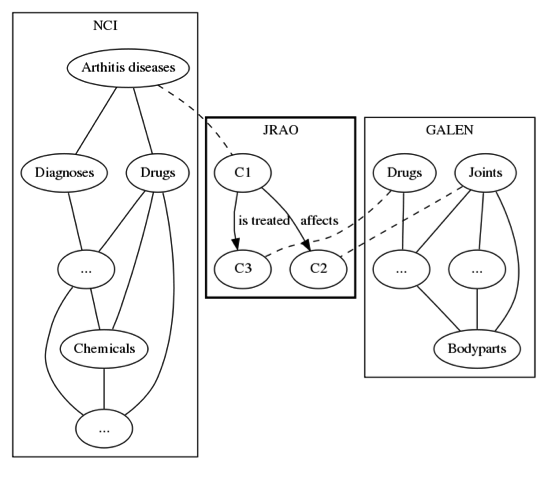
\includegraphics[width=0.6\textwidth]{useCaseOnto3.png}
\caption{JRAO  -- Example for Module Extraction}
\label{JRAO}
\end{center}
\end{figure}


\begin{lstlisting}[basicstyle=\ttfamily,language=dolText,morekeywords={props,ObjectProperty,Class,DisjointUnionOf,SubClassOf,Characteristics,Transitive,Asymmetric,SubPropertyOf,DisjointClasses,EquivalentTo,inverse,only,forall,iff,if,or,exists,distributed,extract},escapechar=@,mathescape]
library GalenModule
logic OWL
ontology myGalen = 
  http://purl.bioontology.org/ontology/GALEN extract Drugs, Joints, Bodyparts
end

module myGalenIsAModule : myGalen of http://purl.bioontology.org/ontology/GALEN 
  for Drugs, Joints, Bodyparts
end
\end{lstlisting}
 


\section{Use Case Onto-4: Interoperability Between Closed-World Data and Open-World Metadata}
Data collection has become easier and much more widespread over the years. This data has to be 
assigned a meaning somehow, which occurs traditionally in the  form of metadata annotations. For 
instance, consider geographical datasets derived from satellite data and raw sensor readings. 
Current implementations in, e.g., ecological economics\cite{bagstad_aries_2011} require manual 
annotation of datasets with the information relevant for their processes. While there have been 
attempts to standardize such information\cite{european_comission_inspire_2014}, metadata for 
datasets of simulation results are more difficult to standardize. Moreover, it is 
resource-consuming to link the data to the metadata, to ensure the metadata itself is of good 
quality and consistent, and to actually exploit the metadata when querying the data for data 
analysis. 

The data is usually represented in a database or RDF triple store, which work with a \termref{closed world assumption} on the dataset, and are not expressive enough to 
incorporate the metadata `background knowledge', such as the conditions for validity of the physical laws in the model of the object of observation. These metadata 
require a more expressive language, such as OWL or Common Logic, which operate under an open-world semantics. However, it is unfeasible to translate the 
whole large dataset into OWL or first-order logic. To `meet in the middle', it is possible to declare bridge rules (i.e., a mapping layer) that can link the metadata to 
the data. This approach can be used for intelligent data analysis that combines the data and metadata through querying the system. It enables the analysis of the 
data on the conceptual layer, instead of users having to learn the SQL/SPARQL query languages and how the data is stored. There are various tools and theories 
to realize this, which is collectively called Ontology-Based Data Access/Management, see also [OBDA].

The languages for representing the metadata or ontology, for representing the bridge rules or mapping assertions, and for representing the data are different yet 
they need to be orchestrated and handled smoothly in the system, be this for data analytics for large enterprises, for formulating policies, or in silico biology in the 
sciences. 

\DOL  provides the framework for expressing such bridge rules in a systematic way, maintaining these, and building tools for them. 


\section{Use Case Onto-5: Verification of Rules Translating Dublin Core Into PROV}
The Dublin Core Metadata terms, which have been formalized as an RDF Schema vocabulary, developed initially by the digital library community, are less 
comprehensive but more widely used than PROV (cf. Use Case Onto-1). The rules for translating Dublin Core to the OWL subset of PROV (and, with restrictions, 
vice versa) are not known to yield valid instances of the PROV data model, i.e. they are not known to yield OWL ontologies consistent with respect to the OWL axioms that 
capture part of the PROV data model. This may disrupt systems that would like to reason about the provenance of an entity, and thus the assessment of the 
entity's quality, reliability or trustworthiness.
The Dublin Core to PROV ontology translation%
\footnote{\url{http://www.w3.org/TR/2013/NOTE-prov-dc-20130430/}}
  is expressed partly by a symbol mapping and partly by FOL rules. These FOL rules are implemented by CONSTRUCT patterns in the SPARQL RDF query language.%
\footnote{E.g., \url{http://www.w3.org/TR/2013/NOTE-prov-dc-20130430/\#dct-creator}} 
SPARQL has a formal specification of the evaluation semantics of its algebraic expressions, which is different from the model-theoretic semantics of the OWL and RDF Schema languages; nevertheless SPARQL CONSTRUCT is a popular and immediately executable syntax for expressing translation rules between ontologies in RDF-based languages in a subset of FOL.
\DOL  not only supports the reuse of the existing Dublin Core RDF Schema and PROV OWL ontologies as modules of a distributed ontology (= OMS network), but it is also able to support the description of the FOL translation rules in a sufficiently expressive ontology language, e.g. Common Logic, and thus enable formal verification of the translation from Dublin Core to PROV.


\section{Use Case Spec-1: Modularity of Specifications}\label{spec-1}
Often specifications become so large that it is necessary to structure
them in a modular way, for human readability and maintainability, and for more efficient tool support. The lack of a standard for such
modular structuring hinders interoperability among different
development efforts and the reuse of specifications.  \DOL provides a
notion of structured modular specification that is equally applicable
to all \DOL-conforming logical languages.

Structuring pays off even for small specifications. For example, it makes
structuring a simple specification of sorting lists in the 
following way enhances both readability and potential for re-use
of specifications:

\begin{lstlisting}[basicstyle=\ttfamily\footnotesize,language=dolText,morekeywords={sort, ops, refinement, free,spec type, assoc, unit,props,op,spec,refined, via,generated, then,ObjectProperty,Class,DisjointUnionOf,SubClassOf,Characteristics,Transitive,Asymmetric,SubPropertyOf,DisjointClasses,EquivalentTo,inverse,only,forall,iff,if,or,exists,distributed,from},escapechar=@,mathescape]	
library Sorting

%% refinement from abstract sorting to insert sort

logic CASL
%right_assoc __::__
spec TotalOrder =
  sort Elem
  pred __<=__ : Elem * Elem
  forall x,y,z : Elem
  . x <= x                         %(reflexive)%
  . x <= z if x <= y /\ y <= z     %(transitive)%
  . x = y if x <= y /\ y <= x      %(antisymmetric)%
  . x <= y \/ y <= x               %(dichotomous)%
end

spec Nat =
  free type Nat ::= 0 | suc(Nat)
end

spec List =
  Nat
then
  sort Elem
  free type List ::= [] | __::__(Elem; List)
  op count : Elem * List -> Nat
  forall x,y : Elem; L : List
  . count(x,[]) = 0
  . count(x,x :: L) = suc(count(x,L))
  . count(x,y :: L) = count(x,L) if not x=y
end

spec Sorting =
  TotalOrder and List
then
  preds is_ordered : List;
        permutation : List * List
  vars x,y:Elem; L,L1,L2:List
  . is_ordered([])
  . is_ordered(x::[])
  . is_ordered(x::y::L) <=> x<=y /\ is_ordered(y::L)
  . permutation(L1,L2) <=> (forall x:Elem . count(x,L1) = count(x,L2))
then
  op sorter : List->List
  var L:List
  . is_ordered(sorter(L))
  . permutation(L,sorter(L))
hide is_ordered, permutation
end
\end{lstlisting}

In the last step, the structuring operation of hiding is used to
restrict the specification to an export interface:\cbs 
 predicates \texttt{is\_ordered} and \texttt{permutation} are hidden,\cbe because they
are only auxiliary and need not be implemented.


\section{Use Case Spec-2: Specification Refinements}\label{spec-2}
Formal software and hardware development methods are often used to
ensure the correct function of systems which have safety-critical
requirements or which may not be easily accessible for repair or
replacement.  Examples of such requirements can be found in
safety-critical areas such as medical systems, or in the automotive,
avionics and aerospace industries, as well as in components used by
those industries such as in microprocessor design.

Typically, a requirement specification is refined into a
design specification and then an implementation, often involving
several intermediate steps (see, e.g. the V-model [V-model], although
this does not require formal specification).  There are numerous
specification formalisms in use, including the OMG's SysML language;
moreover, often during development, the formalism needs to be changed
(e.g. from a specification to a programming language, or from a
temporal logic to a state machine). For each of these formalisms,
notions of refinement have been defined and implemented. However, the
lack of a standardized, logically sound language and methodology for
such refinement hinders interoperability among different development
efforts and the reuse of refinements.  \DOL provides the capability to
represent refinement that is equally applicable to all \DOL-conforming
logical languages, and that covers at least the most relevant of the
industrial use cases of specification refinement.

A simple example is the refinement of the (purely declarative) sorting
specification from use case in section \ref{spec-1} into a specification of a particular sorting
algorithm (for simplicity,\cbs insert sort is used for demonstration):\cbe

\begin{lstlisting}[basicstyle=\ttfamily\footnotesize,language=dolText,morekeywords={sort, ops, refinement, free,spec type, assoc, unit,props,op,spec,refined, via,generated, then,ObjectProperty,Class,DisjointUnionOf,SubClassOf,Characteristics,Transitive,Asymmetric,SubPropertyOf,DisjointClasses,EquivalentTo,inverse,only,forall,iff,if,or,exists,distributed,from},escapechar=@,mathescape]	
spec InsertSort = 
  TotalOrder and List
then
  ops insert : Elem*List -> List;
      insert_sort : List->List
  vars x,y:Elem; L:List
  . insert(x,[]) = x::[]
  . insert(x,y::L) = x::insert(y,L) when x<=y else y::insert(x,L)
  . insert_sort([]) = []
  . insert_sort(x::L) = insert(x,insert_sort(L))
 hide insert
end

refinement InsertSortCorrectness =
   Sorting refined via sorter |-> insert_sort to InsertSort
end
\end{lstlisting}
Note that hiding is essential here to make the signatures of
both specifications compatible.\cbs If  the
predicates \texttt{is\_ordered} and \texttt{permutation}
had not been hidden\cbe in the \texttt{Sorting} specification, a refinement would
not have been possible, since \texttt{InsertSort} does not
implement these predicates (and it would be rather artificial
to add an implementation for them).

\medskip

Refinements can be composed. A simple example below illustrates this
by expressing that natural numbers with addition form a monoid, and
that natural numbers can be efficiently represented for implementation
as lists of binary digits, together with several equivalent ways of
composing these refinements.

\begin{lstlisting}[basicstyle=\ttfamily\footnotesize,language=dolText,morekeywords={sort, ops, refinement, free,spec type, assoc, unit,props,op,spec,refined, via,generated, then,ObjectProperty,Class,DisjointUnionOf,SubClassOf,Characteristics,Transitive,Asymmetric,SubPropertyOf,DisjointClasses,EquivalentTo,inverse,only,forall,iff,if,or,exists,distributed,from},escapechar=@,mathescape]	
spec Monoid =
 sort Elem
 ops 0 : Elem;
         __+__ : Elem * Elem -> Elem, assoc, unit 0
end

spec NatWithSuc = %mono
 free type Nat ::= 0 | suc(Nat)
 op __+__ : Nat * Nat -> Nat, unit 0 
 forall x , y : Nat . x + suc(y) = suc(x + y)
 op 1:Nat = suc(0)
end

spec Nat =
  NatWithSuc hide suc
end

spec NatBin =
generated type Bin ::= 0 | 1 | __0(Bin) | __1(Bin)

ops __+__ , __++__ : Bin * Bin -> Bin 
forall x, y : Bin 
 .  0 0 = 0  .  0 1 = 1
 .  not  (0 = 1)  .  x 0 = y 0 => x = y .  not  (x 0 = y 1)  .  x 1 = y 1 => x = y
 .  0 + 0 = 0  .  0 ++ 0 = 1 
 .  x 0 + y 0 = (x + y) 0  .  x 0 ++ y 0 = (x + y) 1
 .  x 0 + y 1 = (x + y) 1  .  x 0 ++ y 1 = (x ++ y) 0 
 .  x 1 + y 0 = (x + y) 1  .  x 1 ++ y 0 = (x ++ y) 0
 .  x 1 + y 1 = (x ++ y) 0  .  x 1 ++ y 1 = (x ++ y) 1 
end

refinement R2 =
 Nat refined via Nat |-> Bin to NatBin
end

refinement R3 =
 Monoid refined via Elem |-> Nat to
 Nat refined via Nat |-> Bin to NatBin
end

refinement R3' =
 Monoid refined via Elem |-> Nat to R2
end

refinement R3'' = 
 Monoid refined via Elem |-> Nat to Nat then R2
end

refinement R3''' = R1 then R2

\end{lstlisting}



\section{Use Case Model-1: Consistency Among UML Diagrams of Different Types}
\label{model-1}

A typical UML model involves diagrams of different types. Such UML models may have intrinsic errors because diagrams of different types may specify conflicting 
requirements. Typical questions that arise in this context are, e.g.,

\begin{itemize}
\item whether the multiplicities in a class diagram are consistent with each other;
\item whether the attributes and operations in a state machine are
available in a class diagram;
\item	  whether the sequential composition of actions in an interaction diagram is justified by an accompanying OCL specification;
\item 	whether cooperating state machines comply with pre-/post-conditions and invariants;
\item 	whether the behavior prescribed in an interaction diagram is realizable by several state machines cooperating according to a composite structure diagram.
\end{itemize}
Such questions are currently hard to answer in a systematic manner. One method to answer these questions and find such errors is a check for semantic 
consistency. Under some restrictions, the proof of semantic consistency can be (at least partially) performed using model-checking tools like Hugo/RT \cite{knapp-wuttke:models06wsh:2007}. 
Once a formal semantics for the different diagram types has been chosen (see, e.g. \cite{knapp-mossakowski-roggenbach:corr:2014}), it is possible to use \DOL to specify in which 
sense the diagrams need to be consistent, and check this by suitable tools.


\ssclause{The ATM Example}
\label{sec:atm-example}

\cbs The ATM example, which illustrates model-driven development using UML,
is taken from \cite{knapp-mossakowski-roggenbach:corr:2014}.  The example involves\cbe
the design of a traditional automatic teller machine (ATM) connected
to a bank. For simplicity, \cbs the example focuses
 on the ATM's processing of card and PIN entry actions.\cbe  
After entering the card, one has three
trials for entering the correct PIN (which is checked by the
bank). After three unsuccessful trials the card is kept.

\begin{figure}[!Ht]
\centering
\subfigure[Interaction\label{fig:interaction}]{%
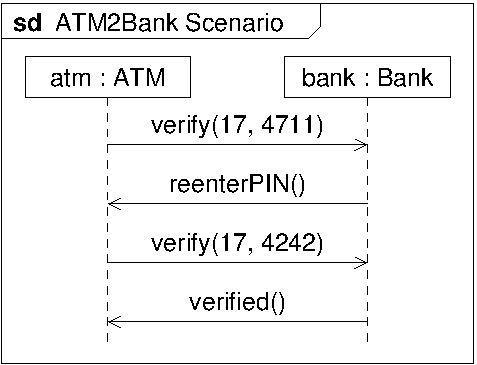
\includegraphics[scale=.5]{illustrations/uml/sd-atm2bank.pdf}
%  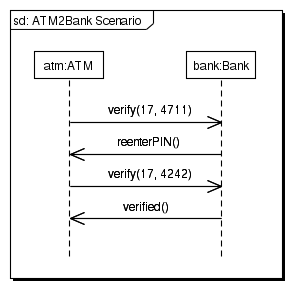
\includegraphics[trim=6 6 6 6,clip,scale=0.65]{illustrations/uml/scenario.png}%\\[-1.5ex]
}
\hspace*{0.5cm}
\subfigure[Composite structure\label{fig:system}]{%
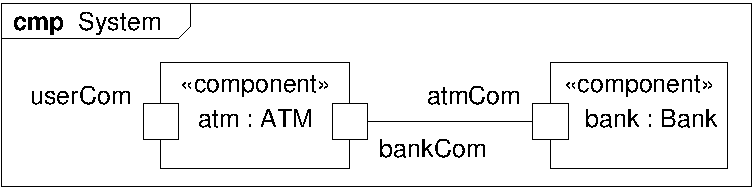
\includegraphics[scale=.5]{illustrations/uml/cmp-system.pdf}
%  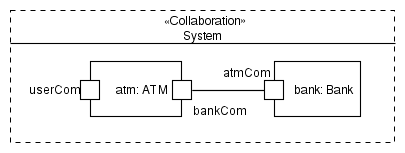
\includegraphics[trim=6 6 6 6,clip,scale=0.65]{illustrations/uml/system.png}%\\[-1.5ex]
}
\\
\subfigure[Protocol state machine\label{fig:psm}]{%
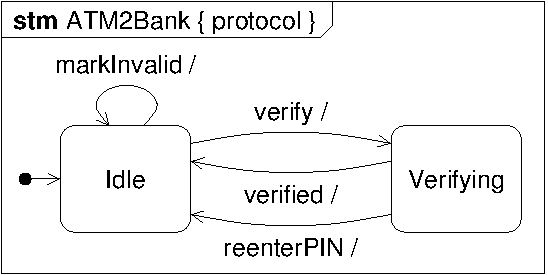
\includegraphics[scale=.5]{illustrations/uml/stm-atm2bank-protocol.pdf}
%  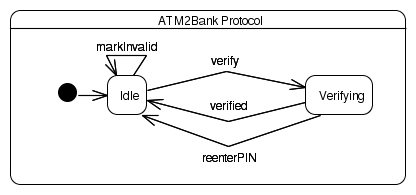
\includegraphics[trim=6 6 6 6,clip,scale=.65]{illustrations/uml/protocol.png}%\\[-1.5ex]
}
\hspace*{0.4cm}
\subfigure[Interfaces and components\label{fig:class}]{%
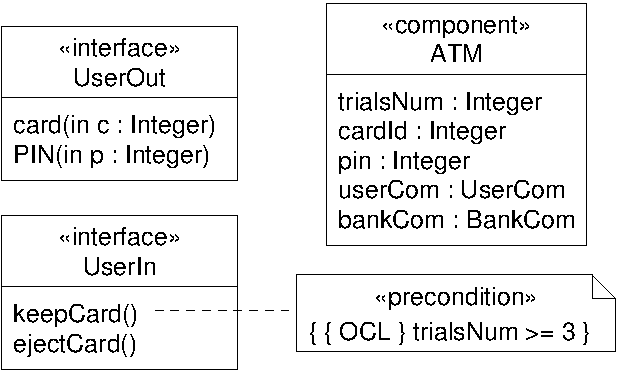
\includegraphics[scale=.5]{illustrations/uml/pkg-components.pdf}
%  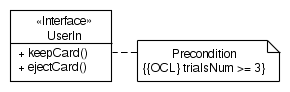
\includegraphics[trim=6 6 6 6,clip,scale=0.65]{illustrations/uml/interfaceWithOCL.png}%\\[-1.5ex]
}
\\
\subfigure[State machine\label{fig:state-machine}]{%
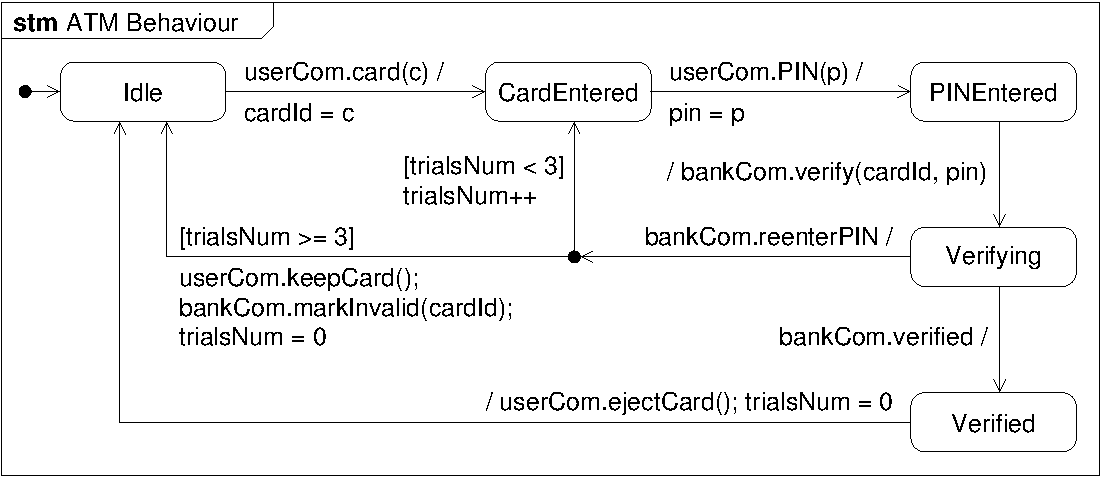
\includegraphics[scale=.5]{illustrations/uml/stm-atm-behaviour.pdf}
%  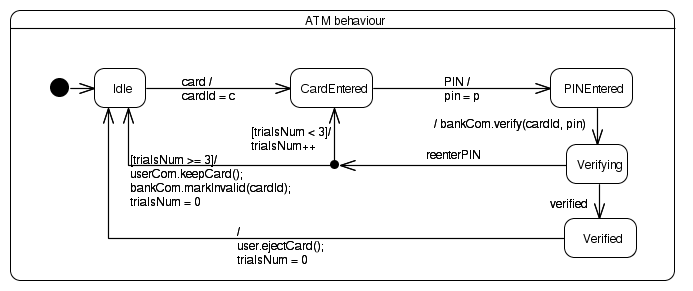
\includegraphics[trim=6 6 6 6,clip,scale=0.65]{illustrations/uml/atm-behaviour.png}%\\[-1.5ex]
}
\vspace*{-1.5ex}
\caption{ATM example}\label{fig:atm-example}
\end{figure}

Figure~\ref{fig:interaction} shows a possible \emph{interaction}
between an \uml{atm} and a \uml{bank} object, which consists of
four messages: the \uml{atm} requests the \uml{bank} to \uml{verify}
if a card and PIN number combination is valid, in the first case the
\uml{bank} requests to reenter the PIN, in the second case the
verification is successful.  This interaction presumes that the system
has an \uml{atm} and a \uml{bank} as objects. This can, e.g., be
ensured by a \emph{composite structure diagram}, see
Fig.~\ref{fig:system}, which -- among other things -- specifies the
objects in the initial system state.  Furthermore, it specifies that
the communication between \uml{atm} and \uml{bank} goes through the
two ports \uml{bankCom} and \uml{atmCom} linked by a connector.  The
communication protocol on this connector is captured with a
\emph{protocol state machine}, see Fig.~\ref{fig:psm}.  The protocol
state machine fixes in which order the messages \uml{verify},
\uml{verified}, \uml{reenterPIN}, and \uml{markInvalid} between
\uml{atm} and \uml{bank} may occur.  Figure~\ref{fig:class} provides
structural information in form of an interface specifying what is
provided at the \uml{userCom} port of the \uml{atm} instance. An
interface is a set of operations that other model elements have to
implement. In our case, the interface is described in a \emph{class
  diagram}. Here, the operation \uml{keepCard} is enriched with the
OCL constraint \uml{trialsNum >= 3}, which refines its semantics:
\uml{keepCard} can only be invoked if the OCL constraints holds.

Finally, the dynamic behavior of the \uml{atm} object is specified by
the \emph{behavioral state machine} shown in
Fig.~\ref{fig:state-machine}. The machine consists of five states
including \uml{Idle}, \uml{CardEntered}, etc.  Beginning in the
initial \uml{Idle} state, the user can \emph{trigger} a state change
by entering the \uml{card}. This has the \emph{effect} that the
parameter \uml{c} from the \uml{card} event is assigned to the
\uml{cardId} in the \uml{atm} object (parameter names are not shown on
triggers). Entering a \uml{PIN} triggers another transition to
\uml{PINEntered}.  Then the ATM requests verification from the bank
using its \uml{bankCom} port.  The transition to \uml{Verifying} uses
a \emph{completion event}: No explicit trigger is declared and the
machine autonomously creates such an event whenever a state is
completed, i.e., all internal activities of the state are finished (in
our example there are no such activities).  If the interaction with
the bank results in \uml{reenterPIN}, and the \emph{guard}
\uml{trialsNum < 3} is true, the user can again enter a \uml{PIN}.


The ATM example in Fig.~\ref{fig:atm-example} consists of five different
models, which naturally form a network. Coherence of this network
is expressed as its consistency.\cbs 
It is assumed that XMI representations\cbe of the
relevant UML models have been stored at
\url{http://www.example.org/uml/}, that is under URL
\url{http://www.example.org/uml/xxx.xmi}, where \url{xxx} is
determined as follows:\medskip

\begin{tabular}{|l|l|l|}\hline
\textbf{Figure} & \textbf{\texttt{xxx}} & \textbf{diagram type}\\\hline
Fig.~\ref{fig:interaction} & sd & sequence diagram\\\hline
Fig.~\ref{fig:system} & cmp & composite structure diagram\\\hline
Fig.~\ref{fig:psm} & psm & protocol state machine\\\hline
Fig.~\ref{fig:class} & cd & class diagram\\\hline
Fig.~\ref{fig:state-machine} & stm & state machine\\\hline
\end{tabular}

\begin{lstlisting}[basicstyle=\ttfamily,language=dolText,morekeywords={props,ObjectProperty,Class,DisjointUnionOf,SubClassOf,Characteristics,Transitive,Asymmetric,SubPropertyOf,DisjointClasses,EquivalentTo,inverse,only,forall,iff,if,or,exists,distributed,refinement,library,via,network,entailment,entails,refined,consistent},escapechar=@,mathescape]
%prefix( :      <http://www.example.org/uml/>
         uml:   <http://www.uml.org/spec/UML/>
         log:   <http://purl.net/DOL/logics/> )%
                %% descriptions of logics ...
library ATM

view cd2stm = cd to { atm hide along stm2cd} end
view cd2psm = cd to { psm hide along psm2cd} end
network ATM_network = %consistent
                      cd, stm, psm, cmp,
                      cd2stm, cd2psm, abstract_to_concrete_atm
entailment atm in ATM_network entails sd
network Some_refined_ATM_network = ...
refinement r = ATM_network refined to Some_refined_ATM_network
entailment e = Some_refined_ATM_network entails ATM_network
\end{lstlisting}
Here, \texttt{abstract\_to\_concrete\_atm} is defined in the next
section, and \texttt{stm2cd} and \texttt{psm2cd} are suitable logic
projections extracting the classes, attributes and operations from a
(protocol) state machine, delivering a class diagram.

\section{Use Case Model-2: Refinements Between UML Diagrams of Different Types, and Their Reuse}
\label{model-2}

A problem is a lack of reusability of refinements: Consider a controller for an elevator, which is specified with a UML protocol state machine, enriched with UML 
sequence diagrams and OCL constraints. Assume further that this model is not directly implemented, but first refined to a UML behavior state machine (which then 
can be automatically or semi-automatically transformed into some implementation using standard UML tools). However, there is no standardized language to 
express, document and maintain the refinement relation itself (UML only allows very simple refinements, namely between state machines). This hinders both the 
reuse of such refinements in different contexts, as well as the interoperability of tools proving such refinements to be correct. \DOL  
addresses these problems by providing a standardized notation with formal semantics for such refinements. Refinements expressed in this language could, e.g., be 
parameterized and reused in different contexts.

\cbs This can be illustrated based on the state
machine of the \uml{atm}, shown in Fig.~\ref{fig:state-machine}, which is a  
refinement of the protocol state machine in Fig.~\ref{fig:psm}. This can be stated as follows in \DOL.\cbe 
\footnote{\cbs  It is assumed that XMI representations of the relevant UML models have been 
stored at \url{http://www.example.org/uml/},
e.g.\ \url{http://www.example.org/uml/atm.xmi} \cbe} 


\begin{lstlisting}[basicstyle=\ttfamily,language=dolText,morekeywords={props,ObjectProperty,Class,DisjointUnionOf,SubClassOf,Characteristics,Transitive,Asymmetric,SubPropertyOf,DisjointClasses,EquivalentTo,inverse,only,forall,iff,if,or,exists,distributed,refinement,library,via},escapechar=@,mathescape]
refinement abstract_to_concrete_atm =
  psm refined via translation psm2atm to 
       {  atm with Idle |-> Idle, CardEntered |-> Idle, 
                   PINEntered |-> Idle, Verified |-> Idle, 
                   Verifying |-> Verifying 
          hide card, PIN   }
end
\end{lstlisting}

The refinement uses an abstraction of the \uml{atm}, expressed by the
translation via symbol map \texttt{Idle |-> Idle, CardEntered |-> Idle, PINEntered |-> Idle, Verified |-> Idle, Verifying |-> Verifying}, resulting in a two-state machine. Moreover, some detail of the \uml{atm} is hidden using
\syntax{hide}. Then, the protocol state machine can be refined to
the thus abstracted \uml{atm}.

\section{Use Case Model-3: Coherent Semantics for Multi-Language Models}
\label{model-3}
	
Often a single problem area within a given domain must be represented using several formalisms, e.g., because of user community requirements, expressiveness or tool support 
and usage. 
Typically the different representations are written by different people using formalisms that are based on different logics. Thus, it is a challenge to maintain 
consistency across the different representations. 
The need for the use of multiple OMS languages, even within the OMG community, is also reflected by the OMG Ontology Definition Metamodel (ODM), which 
provides a number of syntactic transformations between such languages.
One example is the OMG Date-Time Vocabulary (DTV). DTV has been formulated in different languages, each of which addresses different audiences:
\begin{itemize}
\item	 SBVR: business users
\item 	UML (class diagrams and OCL): software implementors
\item 	OWL: ontology developers and users
\item 	Common Logic: (foundational) ontology developers and users
\end{itemize}
With \DOL, one can, e.g.,
\begin{itemize}
\item 	formally relate the different formalizations used for DTV, relate the different formalizations using translations,
\item 	check consistency across the different formalizations (using suitable tools),
\item 	extract sub-modules covering specific aspects, and
\item 	specify the OWL version to be an approximation of the Common Logic version (using a heterogeneous interpretation of OMS).
\end{itemize}
Note that the last point does not specify what information is lost in the approximation. Indeed, \DOL provides the means to specify requirements on the approximation, e.g., that it maximally preserves the information. 

Coming to a \DOL example,
a model like the ATM model developed in section \ref{sec:atm-example} typically is part of an
application context that also contains some common terminology.
This terminology often is specified by an ontology, and then
it is desirable to relate the model to the ontology. Consider
the following financial ontology fragment:

\begin{lstlisting}[basicstyle=\ttfamily,language=dolText,morekeywords={props,ObjectProperty,Class,DisjointUnionOf,SubClassOf,DisjointWith, Irreflexive, Characteristics,Transitive,Asymmetric,SubPropertyOf,DisjointClasses,EquivalentTo,inverse,only,forall,iff,if,or,exists,sort,ops,in,approximate,extract},escapechar=@,mathescape]
ontology myTaxonomy =
  ObjectProperty: owns 
    Characteristics: Irreflexive, Asymmetric

  Class: FinancialIntermediary
    SubClassOf: CorporatePerson 
  Class: CorporatePerson
    SubClassOf: ImmaterialEntity
  Class: ImmaterialEntity
    DisjointWith: MaterialEntity
    SubClassOf: has_part only ImmaterialEntity
  Class: Livestock 	
    SubClassOf: MaterialEntity 
...
end
\end{lstlisting}

\cbs To relate this ontology with the ATM model, 
various aspects need to be taken care of:\cbe
\begin{itemize}
  \item Translating into shared language \cbs (in this case, Common Logic)\cbe
  \item Unifying terminology (Bank vs. FinancialIntermediary)
  \item Connecting related concepts (bank.owns.ATM vs. owns)
  \item Removing irrelevant parts (livestock) 
\end{itemize}

\begin{lstlisting}[basicstyle=\ttfamily\small,language=dolText,morekeywords={props,ObjectProperty,Class,DisjointUnionOf,SubClassOf,DisjointWith, OMS, Characteristics,Transitive,Asymmetric,translation,SubPropertyOf,DisjointClasses,EquivalentTo,inverse,only,forall,iff,if,or,exists,sort,ops,in,approximate,extract,oms,model},escapechar=@,mathescape]
model xmiStateModel = <https://ontohub.org/ATM/state.xmi>

model clStateModel = xmiStateModel with
                     translation UMLState2CL

model xmiClassModel = <https://ontohub.org/ATM/class.xmi>			

model clClassModel = xmiClassModel with 
            translation UMLClass2CL 
            Bank |-> FinancialIntermediary

ontology BigTaxonomy = <https://ontohub.org/ATM/mytaxonmy.owl>			

ontology NoLivestockTaxonomy = BigTaxonomy reject
                               Class: Livestock
						  end

ontology ExtendedTaxonomy = NoLivestockTaxonomy then 
         ObjectProperty FinancialIntermediary.owns.ATM
           SubPropertyOf: owns 
           Domain: FinancialIntermediary 
           Range: ATM
end

ontology clTaxonomy = ExtendedTaxonomy with 
                      translation OWL22CommonLogic

oms JointModel = clStateModel and 
                 clClassModel and 
                 clTaxonomy
end
\end{lstlisting}


\section{Conclusion}
\cbs
In this section, the use cases have been used to illustrate many aspects of DOL and how it can be useful in many situations in which different OMS artifacts might be leveraged and augmented to produce broader or more tractable models, ontologies, and specifications.

 \DOL is designed to support of a wide range of formalisms and
provides the ability to specify the basis for formal interoperability even among heterogeneous OMS and OMS networks. \DOL enables the solutions of the problems described in the use cases above. It also enables the development of DOL documents, tools and workflows that 
allow  a better exchange and reuse of OMS. Eventually, this will also lead to better, easier developed and maintained systems based on these OMS.

The next sections present the metalanguage \DOL{}; in particular, the syntax and the model-theoretic semantics. Further, various features of \DOL will be discussed, which  are based on  best practices of modularity  across
 the three areas of ontology design, formal 
specification, and model-driven development.
\cbe



\clauseI{Design Overview} \label{c:design}

%\ednote{replace this section by saying how we respond to the RFP}
%
%\CLnote[type=todo]{Get rid of formal \should/\shall language (e.g.\ in clause headers: \should/\shall applies to conforming implementations anyway, rather than to this standard itself!) – not necessary in an informative clause. TM: I did this in the clause headings, and for the design part also in the clause texts.}
%
%
The purpose of this clause is to briefly describe the 
%purposes of the Distributed Ontology, Modeling and Specification Language (\DOL) and 
 overall guiding principles and constraints of \DOL's syntax and semantics.
%
%\todonote{add somewhere: \DOL is a meta language and can be used with OMS languages of any expressiveness. As a Meta-language, \DOL provides a framework for combining and relating OMS written in specific OMS languages.
%However, \DOL cannot be used for writing new basic OMS.}
%
%\todonote{add ref to annex K}
%
%\section{\DOL requirements}\label{c:req:overview}
%
%\DOL has been designed and developed with several requirements in mind, all arising from its intended role of enabling OMS interoperability. The use of ``{\should}'' in the rest of clause 5 indicates a desired goal but is not required of \DOL (in accordance with Annex H of ISO/IEC Directives -- Part 2).
%
%\CLnote[type=todo]{give quick overview here.  Create clause 5.2 for requirements, and 5.3 for design overview. TM: done}
%
%\subsection{\DOL is free, generally applicable, open, and extensible.}\label{c:req:extensible}
%
%\DOL \should be
%\begin{description}
%\item[free] This \IS \should be freely available for unrestricted use.
%\item[generally applicable] It \should neither be restricted to OMS in a specific domain, nor to foundational OMS, nor to OMS represented in a specific OMS language, nor to OMS stored in any specific repositories.
%\item[open] It \should support mapping, integrating, and annotating OMS across arbitrary internet locations.  It \should make use of existing open standards wherever suitable.  The criteria for extending \DOL (see next item) \should be transparent and explicit.
%\item[extensible] It \should provide a framework into which any existing, and, desirably, any future OMS language can be plugged.
%\end{description}
%
%\DOL \shall be applicable to any OMS language that has a formal, logic-based semantics or a semantics defined by translation to another OMS language with such a formal semantics. The annotation framework of \DOL \should additionally be applicable to the non-logical constructs of such languages. This \IS \todonote[author=Christoph Lange,date=D:201109221211+02'00',type=fyi]{We can afford to say ``shall'' here, as these criteria are really something that we can fully provide} \shall specify formal criteria for establishing the conformance of an OMS language with \DOL.  Annexes \shall establish the conformance of a number of relevant OMS languages with \DOL; a registry shall offer the possibility to add further (also non-standardized) languages:\CLnote[date=D:201201100956+01'00']{John Sowa: Make it modular with a simple core that can run efficiently on small systems, but can grow indefinitely to support as much as anyone could desire.}
%
%\begin{description}
%\item[normative] OWL, Common Logic, RDF Schema\todonote[author=Christoph Lange,date=D:201111021905+01'00']{RIF as well?  See \ticket{16}}
%\item[informative] F-logic,  UML class diagrams, OBO (see appendix~\ref{a:ext-graph} for a longer list)
%\end{description}
%
%\subsection{\DOL is a logic-agnostic metalanguage, in the sense that its constructs can be used for many different logics.}\label{c:req:agnostic}
%
%\CLnote{here and elsewhere: remove ``shall'' from section headers}
%
%\DOL \shall provide syntactic constructs for structuring OMS regardless of the logic their sentences are formalized in. \DOL \should provide syntactic constructs for
%
%\begin{itemize}
%\item basic and structured OMS (and facilities to identify them in a globally unique way),
%\item explicit extraction of modules from existing OMS, \markupcomment[author=Christoph Lange,type=q-aut]{such that, \eg, changes in the OMS can be propagated to the extracted module}{This rather sounds like a use case description to me than like a requirement.  Move it somewhere else?  Where?}.
%\item mappings between OMS (\cf \cref{c:req:links}), including interpretations, relations between OMS and their modules, as well as alignments.
%\end{itemize}
%\DOL \shallnot provide its own constructs for expressing sentences.  Instead, it \shall \textit{inherit} the logical language aspects of conforming OMS languages.  It \should be possible to literally include sentences expressed in such OMS languages in a \DOL OMS.
%
%\DOL \shall provide an initial set of built-in approximation methods and module extraction selectors.  Additionally, it \shall provide a means of referring to approximation methods and module extraction selectors defined externally of this \IS.\todonote[author=Christoph Lange,date=D:201111030047+01'00',type=fyi]{In practice we will use IRIs for that purpose.}
%
%\DOL \shall provide an initial vocabulary for expressing relations in correspondences (as part of alignments between OMS).  Additionally, it \shall provide a means of reusing relation types defined externally of this \IS.
%
%\DOL \shallnot provide an annotation vocabulary, i.e.\ it \shall neither provide annotation properties nor datatypes to be used with literal annotation objects. Instead, an informative annex \shall recommend existing annotation vocabularies for use with \DOL.
%
%\subsection{\DOL has user- and machine-readable serializations.}
%
%\CLnote[type=q-all]{We need to revise this following the agreement to drop the XML and RDF serializations.}In the interest of wide applicability and tool support, \DOL \should support multiple alternative serializations.  In particular, there \should be a text serialization targeting human readers and writers, as well as serializations optimized for machine processability.
%
%This \IS \shall specify criteria for a serialization to conform with \DOL, and it \shall specify the following conforming serializations:
%
%\begin{itemize}
%\item a human-readable \textbf{text serialization}
%\item a machine-processable \textbf{interchange format}, to be implemented as
%  \begin{description}
%  \item[an XML schema (\DOL XML)] particularly targeting document or form based authoring, validation, as well as translation from and to serializations of existing OMS languages\todonote[author=Christoph Lange,date=D:201204050853+02'00',type=q-all]{I think it's reasonable to call this ``\DOL XML'' instead of ``DIF XML'', as to emphasize the ``brand'' \DOL}, and
%  \item[an RDF vocabulary (\DOL RDF)] particularly targeting interlinking and annotation.
%  \end{description}
%\end{itemize}
%
%The \textbf{text serialization} in particular \shall offer a syntax for abbreviating identifiers of resources within OMS in a way that does not require authors to write down their full global identifiers.
%
%An OMS implemented in \DOL \should be able to comprise parts formalized in any OMS language; any serialization of \DOL \should be able to literally include such parts, regardless of the OMS language serialization they have been written in. \todonote[author=Christoph Lange,date=D:201109200256+02'00',type=fyi]{advanced namespacing is the solution that addresses this requirement} Additionally, an OMS implemented in \DOL \should be able to refer to any external OMS formalized in any OMS language, as long as they can be identified in a globally unique way.
%
%Existing OMS in existing XML serializations (\eg XCL) or text serializations (\eg OWL Manchester Syntax) \should validate as \DOL OMS with a minimum amount of syntactic adaptation. Existing OMS files/documents \should be usable in a \DOL context without the need for modification.
%
%\subsection{\DOL has a well-defined formal, logic-based semantics.}\label{c:req:semantics}
%
%The structural elements and structural mappings of \DOL \should have a formal, logic-based semantics.
%
%This \IS specifies OMS language translations between conforming languages:\todonote[author=Christoph Lange,date=D:201110060000+02'00',type=fyi]{we shall establish the conformance of an initial set of languages with \DOL. As a part of that work we deliver the "onto-logical translation graph" between these languages. Anyone, who wants to establish the conformance of another language with \DOL, has to add a node to the graph, and at least one edge from/to an existing node.}
%
%\begin{itemize}
%\item OMS language translations between their logical language aspects. For any such OMS language translation its properties \should be determined, \eg whether it is a sublogic, a theoroidal translation, etc. \\
%~\todonote[author=Christoph Lange,date=D:201110060000+02'00',type=todo]{meet the requirements of people who combine OWL reasoners with Prolog. Some additional research needed on combining logics that have a model theory with those that don't}
%\item OMS language translations between their structuring language aspects and the structuring language aspect of \DOL.
%\end{itemize}
%\DOL can express the application $T(O)$ of an OMS language translation $T\colon L_1\to L_2$ to an OMS $O$ written in langauge $L_1$\todonote[author=Christoph Lange,date=D:201110060000+02'00',type=fyi]{T shall be identified by a IRI. There might be multiple different possible translations between two languages, \eg two ways of expressing OWL roles in CL (binary predicate vs.\ boolean function).  But in order to free the user from always writing down such IRIs, we shall specify some defaults in our translation graph.}, see the \cbs MOF metaclass \cbe 
%\syntax{Translation} in clause~\ref{c:abstract-syntax}.  \DOL need not be capable of expressing OMS language translations.
%
%\begin{figure}
%  \centering
%  \documentclass{standalone}
\usepackage[T1]{fontenc}
\usepackage[utf8]{inputenc}
\usepackage{fourier}
\renewcommand{\sfdefault}{Myriad-LF}
\usepackage[scaled=.8]{beramono}
% Minion and Myriad fonts – comment these lines if you don't have them!
% (http://lglinux.blogspot.com/2007/09/myriad-and-minion-for-latex.html)
\usepackage[minionint,mathlf]{MinionPro}
\usepackage{tikz}
\usetikzlibrary{shadows,shapes,positioning,arrows}
\tikzstyle{ontoiop}=[font=\sffamily,
    language/.style={circle,draw},
    translation/.style={-stealth'},
    dol/.style={rectangle,rounded corners,draw,align=left},
    import/.style={-o},
]
% Our colors
\definecolor{cl}{RGB}{127,129,209}
\definecolor{owl}{RGB}{138,173,72}
\definecolor{rdfs}{RGB}{232,146,31}
\definecolor{dol}{RGB}{253,246,234}
\definecolor{owlxml}{RGB}{240,251,239}
\definecolor{clif}{RGB}{242,242,251}

\begin{document}
  \begin{tikzpicture}[ontoiop]
    % Common Logic
    \node[label=Common Logic,language,fill=cl] (cl) {};
    % OWL
    \node[label=below:OWL,language,fill=owl,below left=of cl] (owl) {};
    % RDFS
    \node[label=below:RDFS,language,fill=rdfs,below right=of cl] (rdfs) {};
    \draw[translation] (owl) to (cl);
    \draw[translation] (rdfs) to (cl);
  \end{tikzpicture}
\end{document}

%  \caption{Translating two OMS languages into a third
%one}
%\label{f:DOL-translations}
%\end{figure}
%
%For each pair $L_1$ and $L_2$ of OMS languages, OMS language translations $T_1$ and $T_2$ into a common target OMS language $L_T$ \should be specified. (If $L_T$ does not exist, the only way to express a heterogeneous OMS involving $L_1$ and $L_2$ may be to keep the \DOL expression and the individual OMS in $L_1$ and $L_2$.)  These \should be translations into an OMS language that is more expressive than both $L_1$ and $L_2$, such that the union of the images of the translations is a subset of the target OMS language ($T_1(L_1)\cup T_2(L_2)\subseteq L_T$).  \fref{f:DOL-translations} outlines such an example, where Common Logic serves as the common target for OWL and RDF Schema, as it is more expressive than either of them.\todonote[author=Christoph Lange,date=D:201110060000+02'00',type=fyi]{In the context of that, specify when a document/an OMS conforms with \DOL.}  If such a target OMS language or suitable translations do not yet exist, translations into a less expressive language may be specified as an alternative, such that the intersection of the images of the translations forms a subset of the target language ($T_1(L_1)\cap T_2(L_2)\subseteq L_T$), which \should be as large as possible.  For example, an OMS language that is more expressive than both Common Logic and F-Logic does not yet exist; therefore, it would be possible to specify translations into the first-order logic subset of either OMS language.
%
%
%
%Reductions of \DOL to conforming OMS languages, as well as approximations of \DOL in conforming OMS languages, are specified.  This is to ensure that OMS that have originally been written in \DOL can be reused and extended in the respective target OMS languages. While approximations are desirable that preserve as much information from the \DOL OMS as the logic underlying the target OMS language is capable of expressing (possibly after a suitable OMS language translation), there \should at least be a trivial reduction that throws away all syntactic constructs of the \DOL OMS that are not syntactic constructs in the target OMS language. However, those constructs are optionally preserved as annotations in the output (cf. \cref{c:req:annotation} for annotations).
%
%\todonote[author=Christoph Lange,date=D:201110060000+02'00',type=todo]{provide example of integrating two OMS in a single-sorted logic by translating into many-sorted logic, where only many-sorted logic would guarantee consistency}
%
%\section{\DOL design}
\label{c:design:overview}
%
%
\cbs It provides an overview of \cbe the most important and innovative language
constructs of \DOL. Details can be found in clause~\ref{c:abstract-syntax}.

\section{\DOL in a Nutshell}

As the usage scenarios in clause \ref{c:goal} illustrate, the use of multiple OMS may lead to lack 
 of interoperability. The goal of \DOL is to enable users to overcome these interoperability issues by providing a language for representing 
structured OMS and the relations between OMS as part of an OMS network in a semantically well-defined way. One particular challenge that needs to be
addressed is that OMS are written in a wide variety of OMS languages, which differ in style, 
expressivity and logical properties. 
\cbs To address this diversity this specification does \textbf{not} propose a 
``universal'' language that is intended to subsume all the others. Quite the opposite, the authors of this specification embrace
the pluralism of OMS languages, and the purpose of \DOL is to provide means (on a sound and formal semantic basis) to\cbe 
 compare and integrate OMS written in different formalisms. Thus, \DOL is not `yet-another-modeling
language', but a meta-language that is used on top of existing OMS languages. 

The major functions of \DOL are the following: 
\begin{itemize}
		\item \DOL allows the use of OMS in other OMS languages (e.g., UML class diagrams, \CASL, 
		OWL, Common Logic) without requiring any changes. These are called \emph{native OMS}.  
		\item \DOL provides for defining new, \emph{structured OMS} based on existing OMS.\footnote{Native OMS can also use the structuring constructs from their OMS language. However, these structuring constructs are often quite limited, and moreover, they differ from OMS language to OMS language.} \DOL provides a number of operations for this purpose; e.g.,
		it is possible to define a structured OMS $C$ as the union of an OWL
		ontology $A$ and a Common Logic ontology $B$.
		\item \DOL provides for defining connections between two OMS by using 
		\emph{OMS mappings}. \DOL provides a variety of mappings; e.g.,  one can align terminology 
		between different OMS or specify that some OMS is an extension of another. A set of OMS
		and OMS mappings may form together an \emph{OMS network}.
		\item Native OMS inherit their semantics from the underlying OMS languages. The \DOL
		 operations for defining structured OMS, 
		OMS mappings, and OMS networks have a declarative model-theoretic semantics, which is 
		 defined in \cref{c:semantics}.  
\end{itemize}
 
The syntax of \DOL roughly follows these functions; native OMS, the various kind of structured OMS, OMS mappings, and OMS networks are the most important \cbs metaclasses \cbe  of \DOL. 
They (together with importations) form the items in a \emph{\DOL library}.
 





\section{Features of \DOL}\label{c:req:overview}

\DOL is a language enabling OMS interoperability. 
\DOL is
\begin{description}
\item[free] \DOL is freely available for unrestricted use.
\item[generally applicable] \DOL is neither restricted to OMS in a specific domain, nor to foundational OMS, nor to OMS represented in a specific OMS language, nor to OMS stored in any specific repositories.
\item[open] \DOL supports mapping, integrating, and annotating OMS across arbitrary internet locations.  It makes use of existing open standards wherever suitable.  The criteria for extending \DOL (see next item) are transparent and explicit.
\item[extensible] \DOL provides a framework into which any existing, and, desirably, any future OMS language can be plugged.
\end{description}
\DOL is applicable to any OMS language that has a formal, logic-based semantics or a semantics defined by translation to another OMS language with such a formal semantics. The annotation framework of \DOL is additionally applicable to the non-logical constructs of such languages. This \IS specifies formal criteria for establishing the conformance of an OMS language with \DOL.  The annex establishes the conformance of a number of relevant OMS languages with \DOL; a registry shall offer the possibility to add further (\cbs including\cbe non-standardized) languages. 

\DOL provides syntactic constructs for structuring OMS regardless of the logic their sentences are formalized in. 
Since \DOL is a meta-language,  it \textit{inherits} the logical language aspects of conforming OMS languages.  It is possible to literally include sentences expressed in such OMS languages in a \DOL OMS.


\DOL provides an initial vocabulary for expressing relations in correspondences (as part of alignments between OMS).  Additionally, it provides a means of reusing relation types defined externally of this \IS.
\DOL does not provide an annotation vocabulary, i.e.\ it neither provides annotation properties nor datatypes to be used with literal annotation objects.
% Instead, an informative annex recommends existing annotation vocabularies for use with \DOL.
%\CLnote[type=q-all]{We need to revise this following the agreement to drop the XML and RDF serializations.}In the interest of wide applicability and tool support, \DOL  supports multiple alternative serializations.  In particular, there is a text serialization targeting human readers and writers, as well as serializations optimized for machine processability.
%The \textbf{text serialization} in particular offers a syntax for abbreviating identifiers of resources within OMS in a way that does not require authors to write down their full global identifiers.
%An OMS implemented in \DOL can comprise parts formalized in any OMS language; any serialization of \DOL can literally include such parts, regardless of the OMS language serialization they have been written in. \todonote[author=Christoph Lange,date=D:201109200256+02'00',type=fyi]{advanced namespacing is the solution that addresses this requirement} Additionally, an OMS implemented in \DOL can refer to any external OMS formalized in any OMS language, as long as they can be identified in a globally unique way.
%Existing OMS in existing XML serializations (\eg XCL) or text serializations (\eg OWL Manchester Syntax) validate as \DOL OMS with a minimum amount of syntactic adaptation. Existing OMS files/documents are usable in a \DOL context without the need for modification.


%\DOL does not provide a new elementary OMS language, but provides a
% layer to be used on top of existing elementary OMS languages which
% enables OMS engineers to formally express mappings between OMS written
% in different languages and stored at different Web locations. The
% purpose of such OMS networks is enabling a greater extent of
% interoperability between data and services in complex application
% settings.

%
% The following features are essential to the design of this \IS:
%
% \begin{itemize}
% \item \DOL is a language covering OMS modularity, OMS heterogeneity, and
% OMS mapping. In particular, it enables writing structured OMS
% (thereby reusing existing OMS), OMS involving different languages,
% as well as complex mappings and relations between OMS.
% \item \DOL is a declarative language with a formal semantics.
% % for modular OMS that consist of structured OMS that are possibly heterogeneous, i.e.\ are written within the same or in different OMS languages, and made available at different Web locations.
% \item \DOL provides a superset of the modularization, Web awareness and annotation facilities of a number of commonly used OMS languages, including OWL \cite{OWL2}, RDF \cite{RDF}, Common Logic \cite{ISO/IEC 24707:2007} and UML \cite{UML}.\footnote{See \cref{c:req:extensible} for details.}
% \item \DOL is an open, extensible standard that is not restricted to a fixed set of supported OMS language but specifies criteria for any existing or future OMS language to conform with \DOL.
% \item Existing OMS in languages conforming with \DOL remain as they are; they can be enriched with \DOL's modularity and annotation constructs in a non-disruptive way.
% \end{itemize}
%
% \ednote{reformulate this, see RFP}
%
%


\section{OMS Languages}
%\DOL gives interoperability a formal grounding and makes heterogeneous OMS and OMS networks and services based on them amenable to checking of coherence (e.g. consistency, conservativity, intended consequences, and compliance).
 OMS languages are declarative languages for making ontological distinctions formally precise, for modeling a domain in an unambiguous way, or for expressing algebraic specifications of software.   OMS languages are distinguished by the following features:

\begin{description}
\item[Logic] Most commonly, OMS languages are based on a description logic or some other subset of first-order logic, but in some cases, higher-order, modal, paraconsistent and other logics are used.
\item[Modularity] A means of structuring an OMS into reusable parts, reusing parts of other OMS, mapping imported symbols to those in the importing OMS, and asserting additional properties about imported symbols.
\item[Annotation] A means of enabling the attachment of human-readable descriptions to OMS symbols, addressing knowledge engineers and service developers, but also end users of OMS-based services.
\end{description}
Whereas the first feature determines the expressivity of the language and the possibilities for automated reasoning (decidability, tractability, etc.), the latter two facilitate OMS engineering as well as the engineering of OMS-based software.

Acknowledging the wide tool support that conforming established languages such as OWL, RDF, Common Logic, UML, MOF, or \CASL enjoy, existing OMS in these (and any other) conforming languages remain as they are within the \DOL framework. \DOL enhances their modularity and annotation facilities to a superset of the modularity and annotation facilities they provide themselves. 
Using \DOL's modularity constructs to make statements about modules of existing OMS works by making relevant parts of these OMS, e.g., sets of axioms, identifiable, and then referring to these identifiers from \DOL statements.  \DOL's modularity constructs are semantically well-founded within a library of formal relationships between the logics underlying the different supported OMS languages.
General annotation of OMS and their parts works in a similar way.  Here, \DOL does not provide its own annotation constructs, but once\cbs again\cbe \DOL's general mechanism of making things of interest identifiable can be employed.  Once these things have been identified, the actual annotations can be added using external mechanisms such as RDF.
\ednote{Till, is this standoff markup remark up to date? TM: we promise standoff markup at various places, but we never are specific how this can be written in \DOL.\\
CL: I have now emphasized that \DOL itself doesn't do annotation but only identification, whereas annotation is left to RDF.}

\section{\DOL in the Metamodeling Hierarchy}

\DOL uses the metamodeling hierarchy known from model-driven engineering:
$$\xymatrix{
\Text{M4} &&&
\Text{Set \& category theory}\ar@(ul,ur)^{\Text{specified in}} \restore \\
\Text{M3} &
\Text{MOF}\ar@(ul,ur)^{\Text{conforms to}} &
\Text{EBNF}\ar@(ul,ur)^{\Text{conforms to}} &
\Text{Institutions} \ar[u]^{\Text{specified in}}
\\
\Text{M2} &
\Text{\DOL metamodel} \ar[u]^{\Text{conforms to}} \ar[ur]_(0.3){\Text{conforms to}}&
\Text{OMS language metamodel}
\ar[u]_{\Text{conforms to}} \ar[ul]_(0.7){\Text{\ conforms to}} \ar[ur]_{\Text{conforms to}}
&\\
\Text{M1} & 
\Text{\DOL document} \ar[r]^{\Text{contains}} \ar[u]^{\Text{conforms to}}&
\Text{specific OMS}\ar[u]^{\Text{conforms to}}&\\
}$$

The syntax of a \DOL conformant language can be written in MOF or EBNF,
which are self-describing.  The semantics of a \DOL conformant language
is its presentation as an institution. Institutions themselves are
specified in the language of set theory and category
theory.

{In the future, it may be possible to specify the
  semantics of a \DOL conformant language using a semantics-based
  logical framework such as \cbs LF or MMT. Since LF can be specified in
  LF itself, this \cbe{} would close the loop already at
  M3 also for the semantics.}

\section{Semantic Foundations of \DOL}\label{sem-foundations}


A large variety of OMS languages in use can be captured at an abstract level using the concept of 
\emph{institutions}\index{institution} \cite{GoguenBurstall92}.
This allows the development of\cbs \DOL\cbe independently of the particularities of a logical system and to use the notions of institution and  logical language interchangeably. 
%We first introduce the concept of \emph{logic syntax}.
The main idea is to collect the non-logical
symbols of the language in signatures and to assign to each signature the set of sentences that can be formed with its symbols. 
For each signature,\cbs \DOL provides means\cbe for extracting the symbols it consists of, together with their kind.
Institutions also provide a model theory, which introduces semantics for
the language and gives a satisfaction relation between the models and
the sentences of a signature.   
% The only restriction imposed is the
% satisfaction condition, which captures the idea that truth is
% invariant under change of notation (and enlargement of context) along
% signature morphisms. This relies on two further components of
% institutions: the translation of sentences along signature morphisms,
% and the reduction of models against signature morphisms (generalizing
% the notion of model reduct known from logic).

It is also possible to complement an institution with a proof theory,
introducing a derivability relation between sentences, formalized as 
an \emph{entailment system} \cite{Meseguer89}. In particular, this
can be done for all logics that have so far been in use in \DOL.


Since institutions allow the differences between OMS languages to be elided to common abstractions, 
the semantics of basic OMS is presented in a uniform way.  The semantics of structured OMS, 
OMS mappings, OMS networks, and other \DOL expressions is defined using model-theoretic constructions
on top of institutions. 


\section{\DOL Enables Expression of Logically Heterogeneous OMS and Literal Reuse of Existing OMS}
\DOL is a mechanism for expressing logically heterogeneous OMS. It can be used to combine sentences and structured OMS expressed in different conforming OMS languages
and logics into single documents or modules. With \DOL, sentences or structured OMS of previously existing OMS in
conforming languages can be reused by literally including them into a \DOL OMS. A minimum of wrapping constructs and other annotations (e.g., for identifying the language of a sentence) are provided. 
 See the
\cbs MOF metaclass \cbe  \syntax{OMS} in
clause~\ref{c:abstract-syntax}.

A heterogeneous OMS can import several OMS expressed in different
conforming logics, for which suitable translations have been defined
in the logic graph provided in \aref{a:graph} or in an extension to it
that has been provided when establishing the conformance of some other
logic with \DOL.  Determining the semantics of the heterogeneous OMS
requires a translation into a common target language to be applied
(\cf \cref{c:semantics}).  This translation is determined via a lookup
in the transitive closure of the logic graph.  Depending on the
reasoners available in the given application setting, it can, however,
be necessary to employ a different translation.  Authors can express
which one to employ.  \cbs However, \DOL provides default translations, which are 
applied unless the user specifies a translation that deviates from the default. Both default and non-default translations may be combined to multi-step translations.\cbe 

\section{\DOL Includes Provisions for Expressing Mappings Between OMS}\label{c:req:links}

\DOL provides a syntax for expressing mappings between OMS.  One use case illustrating both is sketched in  \fref{f:DOL-mapping}.  OMS mappings supported by \DOL include:
\begin{itemize}
\item imports (particularly including imports that lead to conservative extensions), see the
\cbs MOF metaclasses \cbe  \syntax{OMSRef} and \syntax{ExtensionOMS} in
clause~\ref{c:abstract-syntax}.
\item interpretations (both between OMS and OMS networks), see the
\cbs MOF metaclass \cbe  \syntax{InterpretationDefinition} in
clause~\ref{c:abstract-syntax}.
\item alignments between OMS, see the
\cbs MOF metaclass \cbe  \syntax{AlignmentDefinition} in
clause~\ref{c:abstract-syntax}.
\item mappings between OMS and their modules, see the
\cbs MOF metaclass \cbe  \syntax{ModuleRelDefinition} in
clause~\ref{c:abstract-syntax}.
\end{itemize}
\DOL uses symbol maps to express signature translations in such OMS mappings; see the
\cbs MOF metaclass \cbe  \syntax{SymbolMap} in
clause~\ref{c:abstract-syntax}.

\DOL need not be able to fully represent logical translations but is
capable of referring to them.

\DOL can also be used to combine or merge OMS along such OMS mappings, see
the rule for \syntax{combination} for the \cbs MOF metaclass \cbe 
\syntax{OMS} in clause~\ref{c:abstract-syntax}.

\begin{figure}
  \centering
  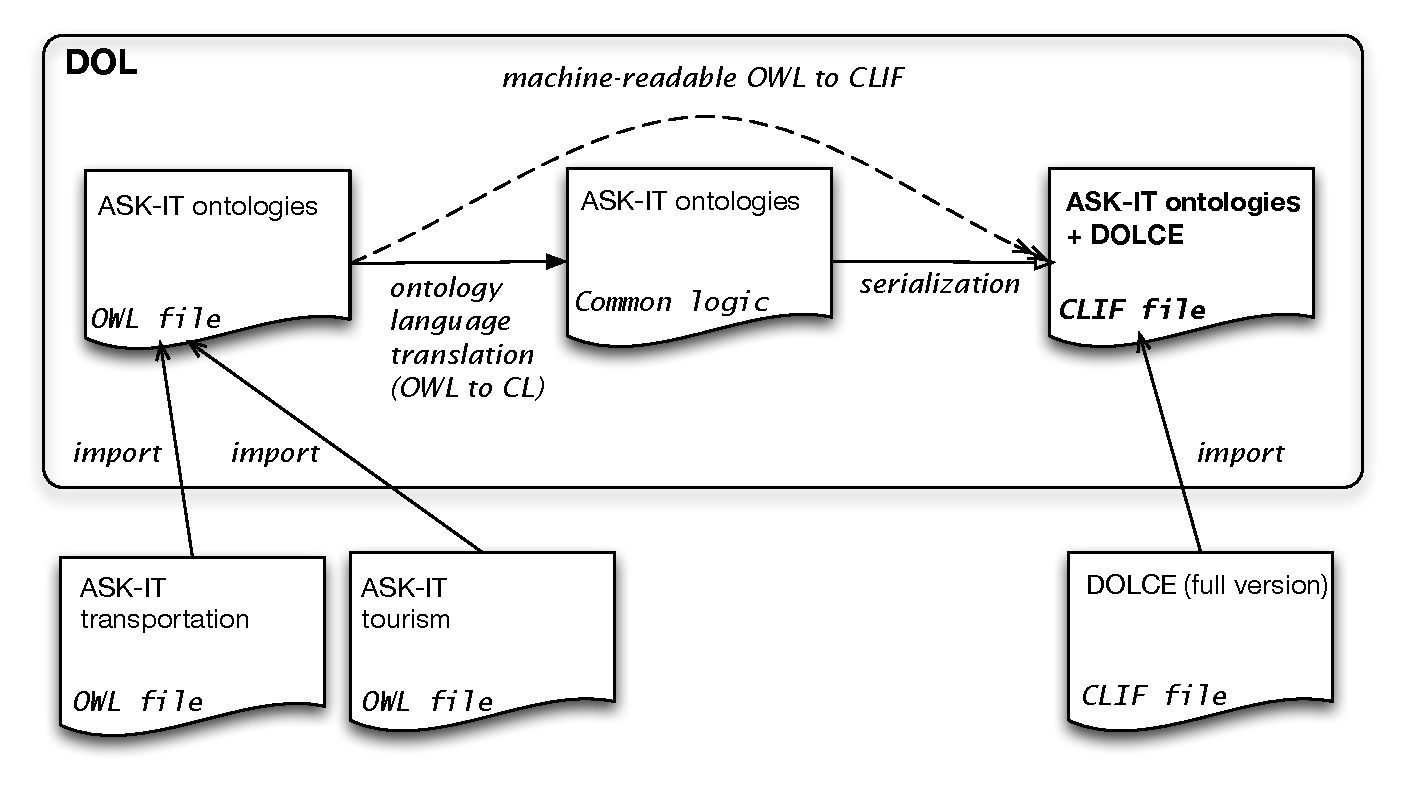
\includegraphics[width=\textwidth]{illustrations/DOLfig.pdf}
  \caption{Mapping between two OMS formulated in different OMS languages}
\label{f:DOL-mapping}
\end{figure}



\section{\DOL Provides a Mechanism for Rich Annotation and Documentation of OMS}\label{c:req:annotation}

\DOL provides a mechanism for identifying anything of relevance in OMS by assigning an IRI to it.  With RDF there is a standard mechanism for annotating things identified by IRIs.  Thus, \DOL supports  annotations in the full generality specified in \cref{c:terms-annotation}.

%A list of recommended RDF vocabularies for annotating OMS is presented in annex \ref{a:dol-onto}.

\clause{\DOL Abstract Syntax}\label{c:abstract-syntax}

\cbs
The clause specifies the \DOL abstract syntax as a MOF metamodel.
In annex~\ref{a:EBNF}, the same abstract syntax is specified using EBNF.
Clause~\ref{a:text-syntax} provides the \DOL concrete syntax, which
uses the metaclasses of the abstract syntax as non-terminals of
an EBNF grammar.
\cbe

\sclause{MOF Metaclasses}

\DOL provides \cbs MOF metaclasses \cbe  for
\begin{itemize}
\item OMS (which can be native OMS in some OMS language, or unions, translations, \cbs closures\cbe, combinations, approximations of OMS, among others)
\item OMS mappings 
\item OMS networks
%\item \red{queries}
\item \DOL libraries (items in these are: definitions of OMS, OMS mappings, and OMS networks, as well as qualifications choosing\cbs (i) the logic,
(2) the OMS language and/or (3) the serialization)\cbe
\item identifiers
\item annotations
\end{itemize}
 
Additionally, the \cbs MOF metaclasses \cbe of the abstract syntaxes
of any conforming OMS languages (\cf \cref{c:conform:logic}) \cbs are
subclasses of the \DOL metaclass \syntax{NativeDocument}.
If a conforming OMS language has a metaclass for basic OMS,
this is a subclass of the metaclass \syntax{BasicOMS}.\cbe

\cbs The following subclauses, one per MOF metaclass, specify the abstract syntax of \DOL in MOF. Additionally, an informative EBNF specification
is given in appendix~ref\cbe{a:EBNF}.\cbe


\sclause{Documents}\label{c:libraries}

\cbs
A \termref{document} (\syntax{Document}) can be a 
\begin{itemize}
\item a \DOL library, or
\item a \syntax{NativeDocument}, which is the verbatim inclusion of an
  OMS written in an OMS language that conforms with \DOL; \cf
  \ref{c:conform:logic}).
\end{itemize}
A \DOL library 
\cbe
 consists of a collection of (named)  OMS, \cbs OMS networks,\cbe{} and mappings between these.  More specifically, a \DOL
library consists of a name, followed by a list of
\syntax{LibraryItem}s.  A \syntax{LibraryItem} is either a
definition of an OMS  (\syntax{OMSDefinition}), 
a mapping between OMS
(\syntax{MappingDefinition}), 
a definition of an OMS network  (\syntax{NetworkDefinition}),
an import of another \DOL library (\syntax{LibraryImport}),
%a definition related to queries 
%(\syntax{QueryRelatedDefinition})
or a \syntax{Qualification} selecting a specific
OMS language, logic and/or syntax that is used to interpret the
subsequent \syntax{LibraryItem}s.  
\cbs A \syntax{LibraryImport} leads to the inclusion of all \syntax{LibraryItem}s of the imported \DOL library into the importing one.\cbe



At the beginning of a \DOL library, one can declare a \syntax{PrefixMap} for abbreviating long IRIs \cbs using CURIEs\cbe; see \cref{c:identifiers} for further details.

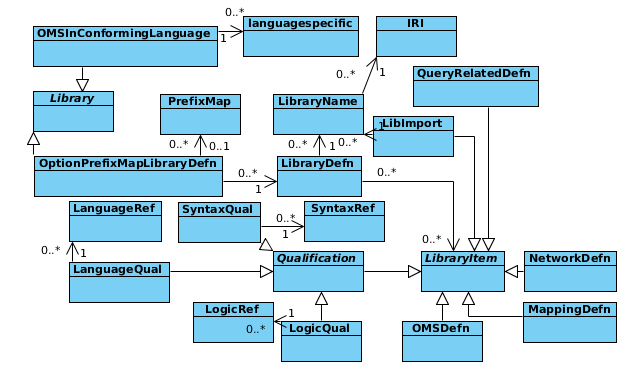
\includegraphics[scale=0.6]{mof/dia/dia0.png}

\sclause{OMS Networks}\label{c:networks}
Inside a \DOL library, one can define OMS networks (\syntax{NetworkDefinition}).
A \syntax{NetworkDefinition} names an
OMS network consisting of  OMS and OMS mappings. OMS networks may build on previously-defined
OMS networks, and they can be used in \syntax{combination}s.  


An OMS network by default also includes all inclusions (\cbs between the extended
and the extending OMS of an\cbe{} \syntax{ExtensionOMS}) between the involved OMS---unless these are
explicitly excluded.

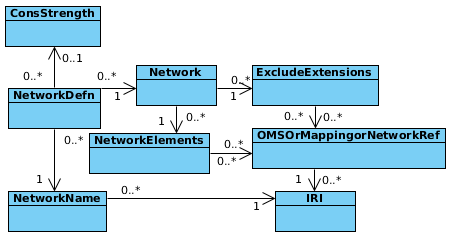
\includegraphics[scale=0.6]{mof/dia/dia1.png}

\sclause{OMS}\label{c:focused-OMS}

An OMS (\syntax{OMS}) can be one of the following:
\begin{itemize}
\item a basic OMS \syntax{BasicOMS} written inline, in a conforming serialization of a conforming OMS 
language (which is defined outside this standard)\footnote{In this place, any OMS in a conforming serialization of a conforming OMS language is permitted.  
However, \DOL's module sublanguage should be given preference over the module sublanguage of 
the respective conforming OMS language; \eg \DOL's extension construct should be preferred over OWL's import construct.},
\item a translation of an OMS into a different signature or OMS
language,
\item a reduction of an OMS to a smaller signature and/or less
expressive logic (that is,
some non-logical symbols are hidden, but the semantic effect of sentences involving these is kept),
\item a module extracted from an OMS, using a restriction signature,
\item an approximation of an OMS, in a subsignature or sublogic, with the effect that sentences not expressible in the subsignature respectively sublogic are replaced with a suitable approximation,
\item a filtering of an OMS, with the effect that some signature symbols and axioms are removed from the OMS,
\item an extension of an OMS with a basic or a closable OMS, optionally named and/or marked as conservative, monomorphic, definitional, weakly definitional or implied (using a \syntax{ConservativityStrength}),
\item a union of several OMS (the major difference between a union and extension is that the members of the unions need to be self-contained OMS, while the extensions may reuse the signature of the extended OMS), 
\item a reference to an OMS existing on the Web,
\item an OMS qualified with the OMS language that is used to express it,
\item a combination of (the OMS contained in) an OMS network (technically, this is a colimit, see \cite{ZimmermanEtAl06}),
\item a \cbs closure\cbe of an OMS, forcing the subsequently declared
  non-logical symbols to be interpreted in a minimal \cbs or maximal\cbe{} way, while the non-logical symbols declared so far are fixed (alternatively, the non-logical symbols to be \cbs minimized/maximized\cbe{} and to be varied can be explicitly declared). Variants of \cbs closure are minimization, \cbe{}
maximization, freeness (minimizing also data sets and equalities on these, \cbs which enables the inductive definition of relations and datatypes), and cofreeness
(enabling the coinductive definition of relations and datatypes).\cbe
%\item the application of a substitution to an OMS.
\end{itemize}
% derived from CASL (see CASL reference manual)
% and HetCASL (see HetCASL summary)

\cbs
Some OMS, namely extensions and \cbs closures\cbe{}, are interpreted relative to a \emph{local environment}.
Roughly speaking, the local environment is the OMS built from all
previously-declared symbols and axioms.

A \syntax{ConservativityStrength} specifies additional relations that may hold
between an OMS and its extension, like conservative or definitional
extension. The rationale is that the extension should not have impact
on the original OMS that is being extended. A \syntax{ConservativityStrength}
might also be applied to a single OMS, which is then implicitly
regarded as an extension of the empty OMS. In this case,
satisfiability (or a similar property) of the OMS is expressed.
\cbe

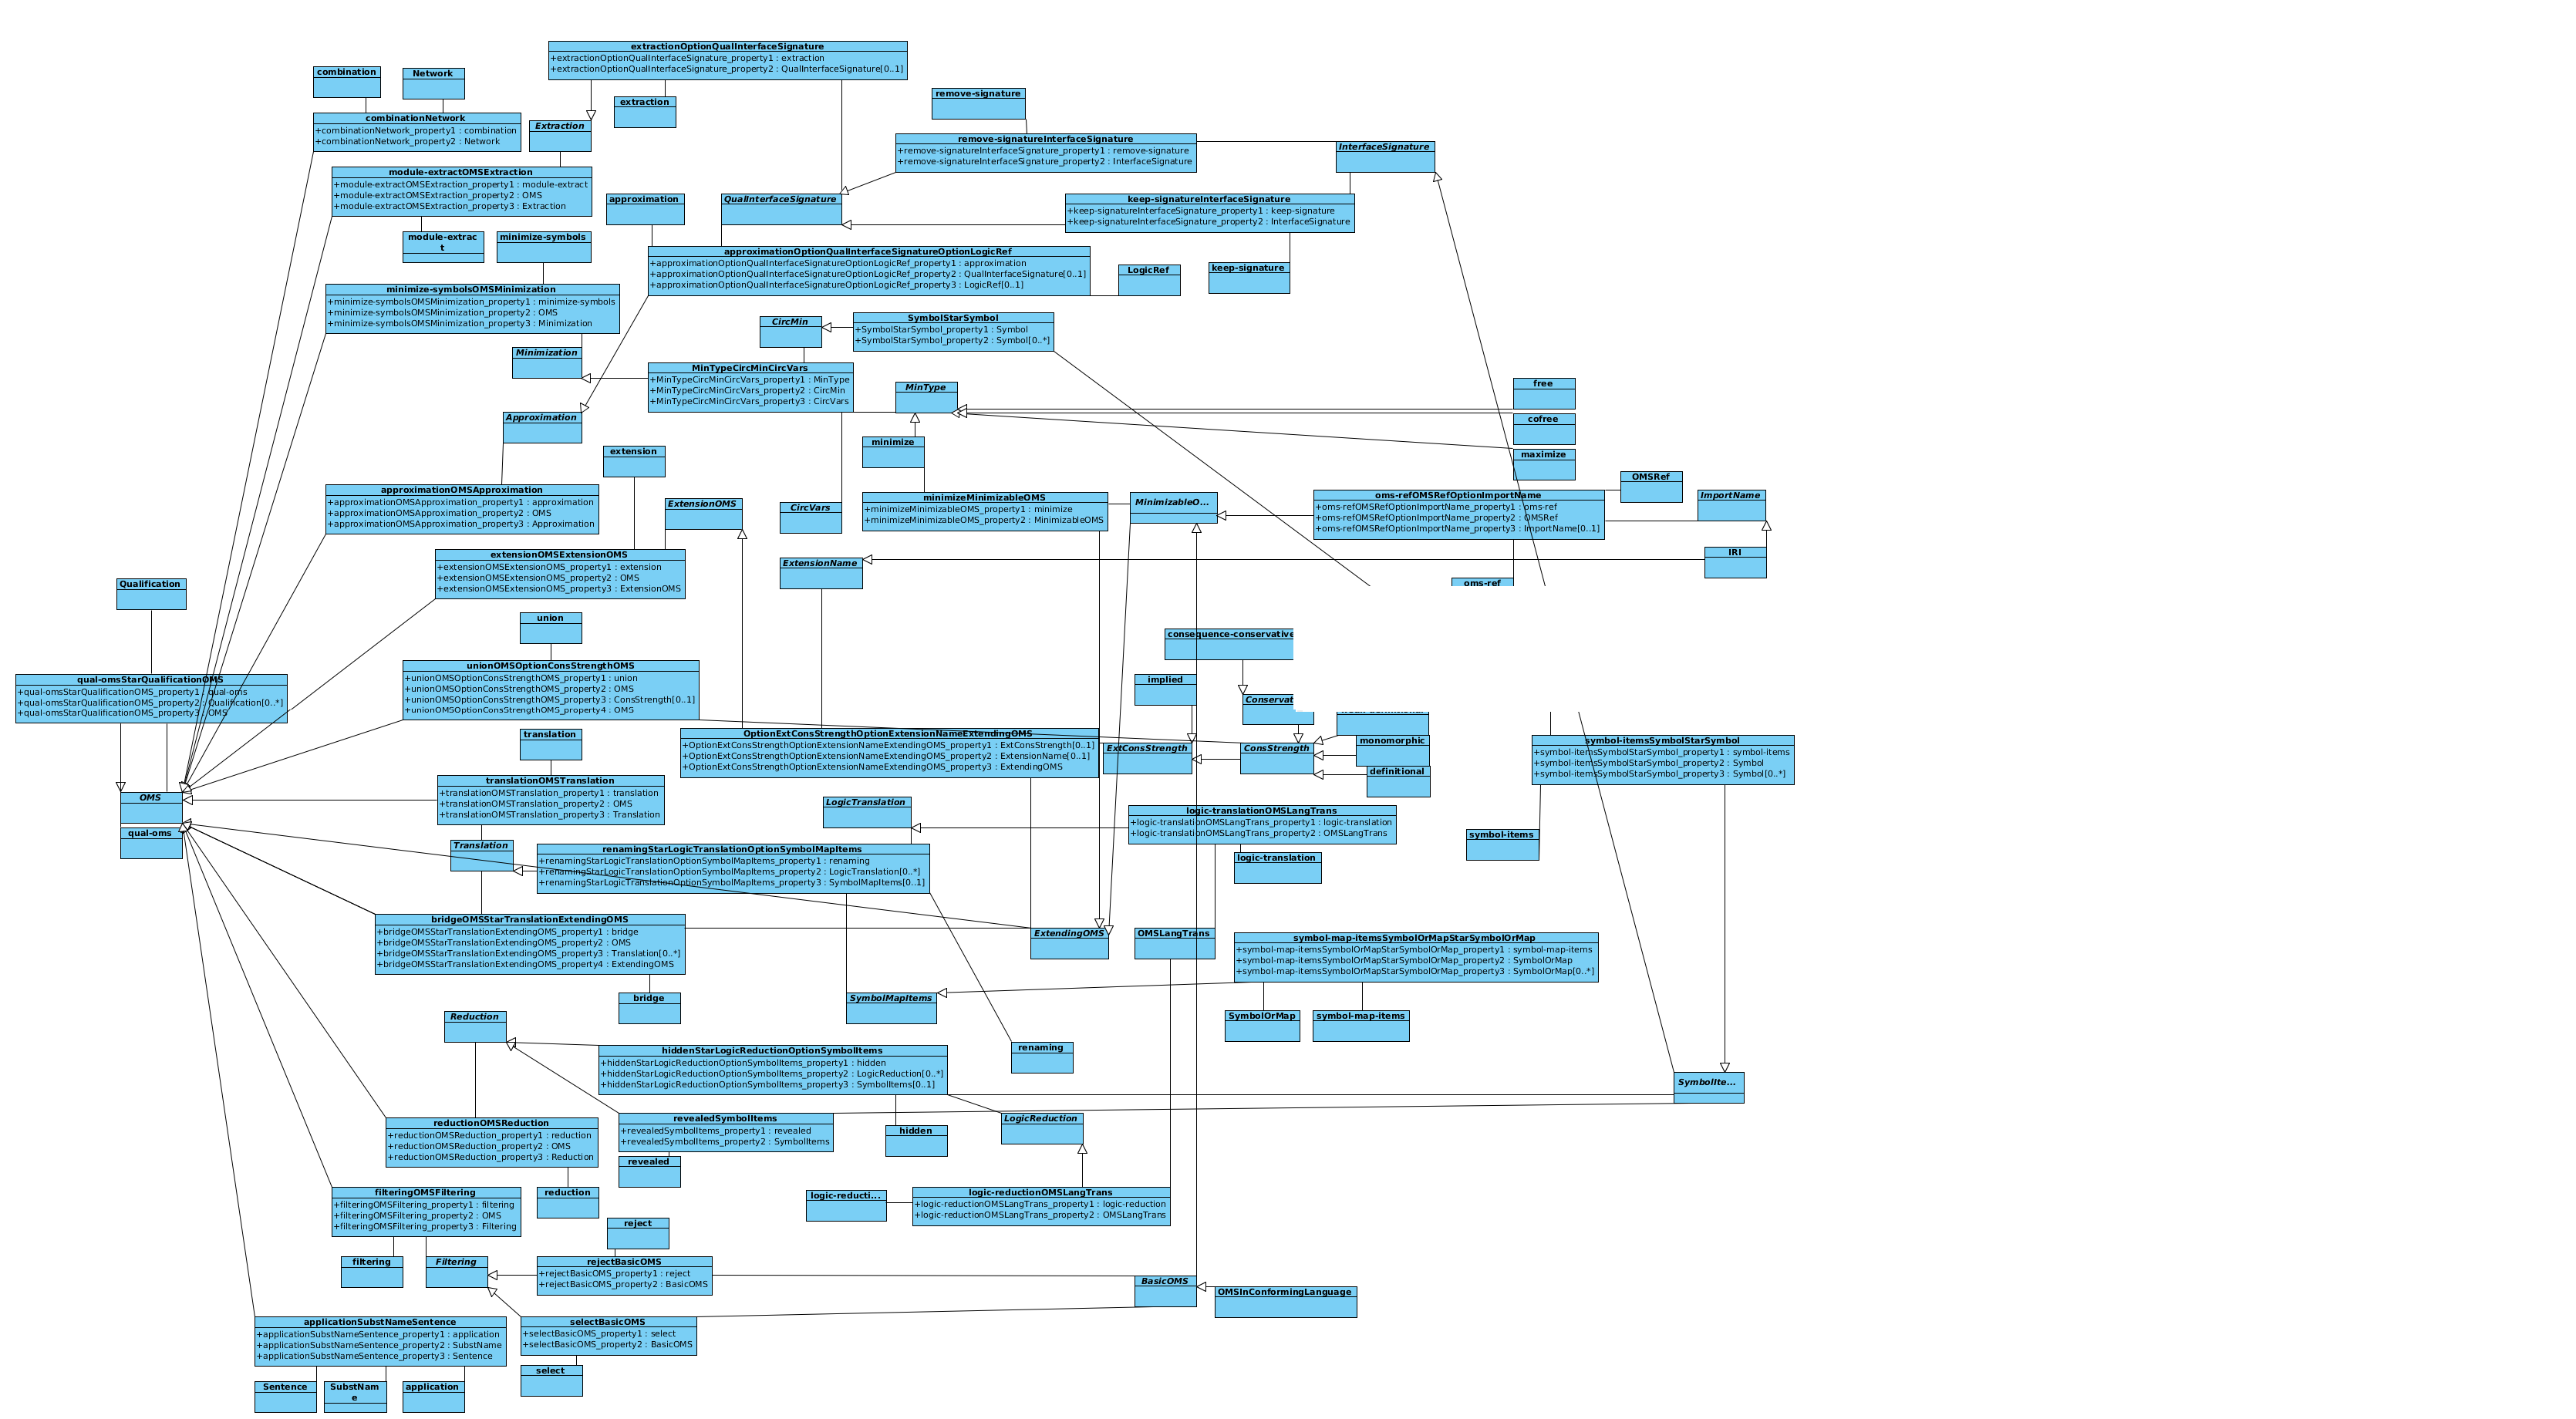
\includegraphics[scale=0.4]{mof/dia/dia2.png}

An OMS definition \syntax{OMSDefinition} names an  OMS.  

It can be
optionally marked as inconsistent, consistent, monomorphic or having a unique model using 
\syntax{ConservativityStrength}. More precisely, \syntax{'consequence-conservative'}
here requires the OMS to have only tautologies as signature-free logical consequences, while \syntax{'not\-consequence-conservative'} expresses that this is not the case. 
\syntax{'model-conservative'}
requires satisfiability of the OMS, \syntax{'not-model-conservative'} its
unsatisfiability.
\syntax{'de\-fi\-nitional'} expresses \cbs that the OMS has a unique model\cbe; this may be interesting for characterizing
OMS (e.g.\ returned by model finders) that are used to describe single models. 

A
\syntax{SymbolItems}, used in an OMS \syntax{Reduction}, is a
list of non-logical symbols that are to be hidden. Also,
an \syntax{OMSLanguageTranslation} denoting a logic projection
can be used a logic reduction to a
less expressive OMS language. A \syntax{SymbolMap}, used in
OMS \syntax{Translation}s,  maps symbols to symbols,
%% \CLnote[type=fyi]{On 2012-07-18 we decided 
%% not to specify lambda-style symbol-to-term mappings for now.  Would be convenient, but specifying its semantics 
%% in an OMS language independent way would require additional institution infrastructure – and the same effect can be 
%% achieved by auxiliary definitional extensions, cf.\ Colore (so promote this, informatively, as a ``best practice''?) TM: Alternatively, we could use a recent notion of institutional monad. This builds an extended signature with all terms. Then one can use ordinary signature morphisms into such extended signatures.} 
%or a logic
%translation. 
An OMS language translation \syntax{OMSLanguageTranslation} 
can be either specified by its name, or be inferred as the \termref{default
translation} to a given target (the source will be inferred as the 
OMS language of the current OMS).

\toleft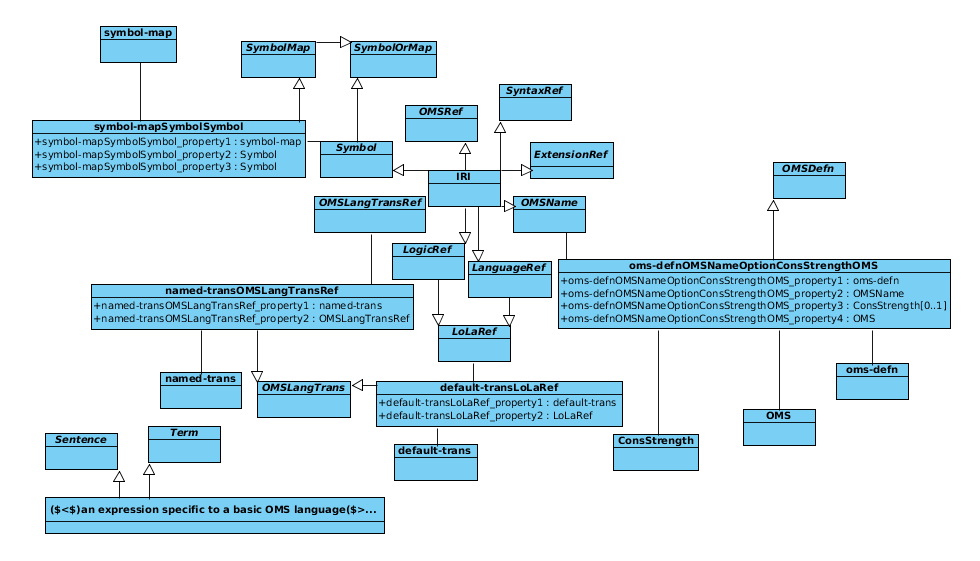
\includegraphics[scale=0.6]{mof/dia/dia3.png}

\sclause{OMS Mappings}\label{c:oms-mappings}

An OMS mapping provides a connection between two OMS. An OMS mapping definition is the definition of 
either a named interpretation (\syntax{InterpretationDefinition}, \syntax{Entailment} or 
\syntax{EquivalenceDefinition}), a named declaration of the  relation between a module of an OMS and the whole 
OMS (\syntax{ModuleRelDefinition}), or a named \termref{alignment} (\syntax{AlignmentDefinition}).

The \syntax{SymbolMap} in an interpretation always must lead to a signature morphism; a proof 
obligation expressing that the (translated) source OMS logically follows from the target OMS is 
generated.  An entailment is a variant where all symbols are mapped identically, while an 
equivalence states that the model classes of two OMS are in bijective correspondence.

Interpretations, entailments and equivalences between OMS networks are also possible. An 
interpretation between OMS networks has to specify both a mapping between the nodes of the OMS 
network, as well as, for each node, a symbol map from the OMS of that node to the target OMS to 
which it is mapped.
%\ednote{In equivalences between OMS networks, should we allow for node mappings 
%as well? In  \cite{MossakowskiTarlecki09}, this is allowed.
%--- No, since we do not allow for signature morphisms either.}


In contrast to this functional style of mapping symbols, an alignment provides a relational 
connection between two OMS,  using a set of \syntax{Correspondence}s. Each correspondence may relate 
some OMS non-logical symbol to another one (possibly given by a term) with an optional confidence 
value. Moreover, the relation between the two non-logical symbols can be explicitly
specified (like being equal, or only being subsumed) in a similar way to the Alignment API \cite{AlignmentAPI}. 
The relations that can be used in a correspondence are equivalence, disjointness, subsumption, membership (the last two with a
variant for each direction) or a user-defined relation that is stored in a registry and must be prefixed with
\url{http://www.omg.org/spec/DOL/correspondences/}.
A default correspondence can be used; it is applied to all pairs of non-logical symbols with 
the same local names. The default relation in a correspondence is equivalence, unless  a different 
relation is specified in a surrounding 
'CorrespondenceBlock'.
Using an \syntax{AlignmentCardinality}, left and right injectivity and totality of the
\termref{alignment} can be specified (the default is left-injective, right-injective, left-total  and right-total).
With \syntax{AlignmentSemantics}, different styles of networks of aligned ontologies (to be interpreted in 
a logic-specific way) of alignments can be specified: whether a single domain is assumed, all domains are embedded into a global domain,
or whether several local domains are linked (``contextualized'') by relations.

A \syntax{ModuleRelDefinition} declares that a certain OMS
actually is a module of some other OMS with respect
to the \syntax{InterfaceSignature}.

\toleft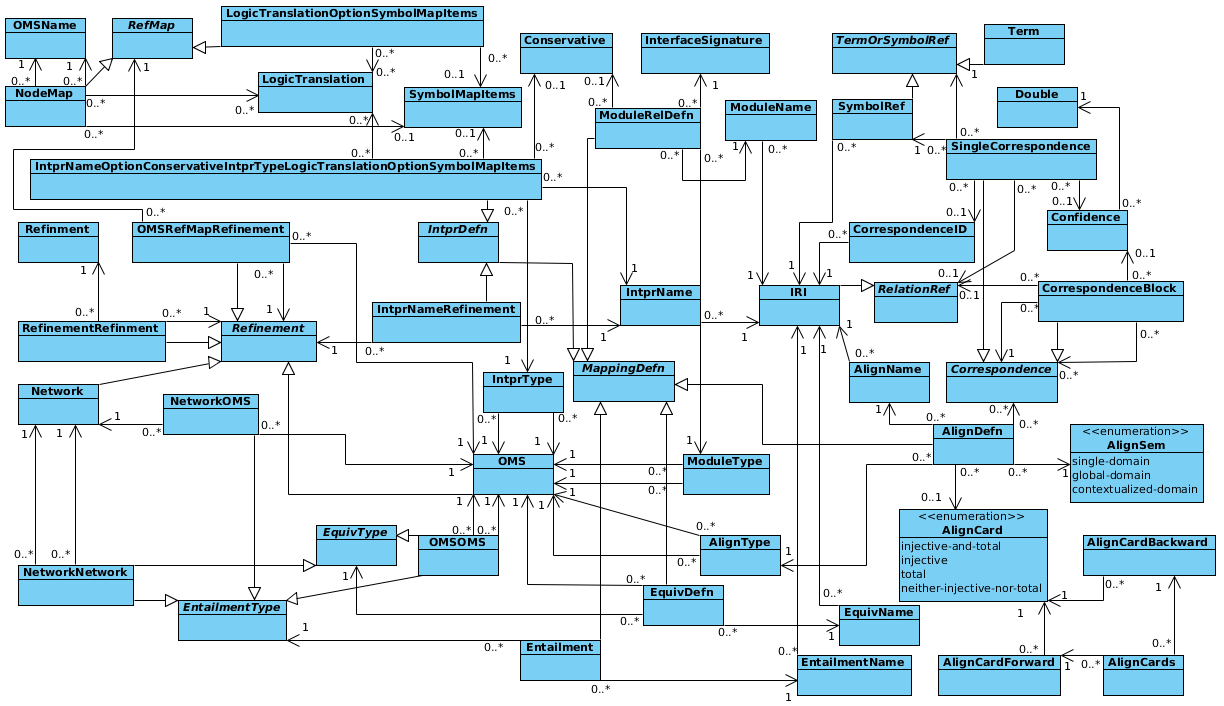
\includegraphics[scale=0.4]{mof/dia/dia4.png}


A symbol map in an interpretation is \required to cover all non-logical symbols of the source OMS; 
the semantics specification in \cref{c:semantics} makes this assumption. ({Mapping a 
non-logical symbol twice is an error. Mapping two source non-logical symbols to the same target 
non-logical symbol is legal, this is a non-injective OMS mapping.})

%Alignments 


%%%%%%%%%%%%%%%%%%%%%%%%%%%%%%%%%%%%%%%%%%%%%%%%%%%%%%%%%%%%%%%%%%%%%%%%

%~\CLnote{some text that was left over here, but I don't recall what we meant by it: recommendations for dealing with OMS language dialects}

\sclause{Identifiers}\label{c:identifiers}

This section specifies the abstract syntax of identifiers of \DOL OMS and their elements.

\ssclause{IRIs}\label{c:iris}

In accordance with best practices for publishing OMS on the Web, identifiers of OMS and their 
elements \should not just serve as \emph{names}, but also as \emph{locators}, which, when 
dereferenced, give access to a concrete representation of an OMS or one of its elements.  (For the 
specific case of RDF Schema and OWL OMS, these best practices are documented in 
\cite{W3C:NOTE-swbp-vocab-pub-20080828}.  The latter is a specialization of the linked data 
principles, which apply to any machine-processable data published on the Web 
\cite{BernersLee:LinkedData2006}.)  It is recommended that publicly accessible \DOL OMS be published 
as linked data.

%\todonote[type=q-aut,author=Christoph Lange]{Does this motivation/justification sound reasonable to 
%you? --- Yes.}
Therefore, in order to impose fewer conformance requirements on applications, \DOL requires the use of
 IRIs for identification per \nisref{IETF/RFC 3987:2005}.
  It is \recommended that \DOL libraries use 
IRIs that translate to URLs when applying the algorithm for mapping IRIs to URIs specified in 
\nisref{IETF/RFC 3987:2005, Section 3.1}.  \DOL descriptions of any element of a \DOL library that is 
identified by a certain IRI \should be \emph{located} at the corresponding URL, so that agents can 
locate them.  As IRIs are specified with a concrete syntax only in \nisref{IETF/RFC 3987:2005}, \DOL 
adopts the latter into its abstract syntax as well as all of its concrete syntaxes 
(serializations).
%\CLnote[type=q-all]{I meant to say: for IRIs, the abstract syntax is the same as 
%the concrete syntax.}.

%% We don't do "semantic namespaces" for now.  (Agreed in 2012-02-23 meeting)
% For identification, \DOL preferably employs IRIs that have the following three components:\footnote{This IRI syntax has originally been designed by Florian Rabe and Michael Kohlhase \cite{Rabe:MMT2011}, independently from this \IS.\todonote[type=todo,author=Christoph Lange]{if we leave this reference in place, we might additionally refer to the paper that describes the semantics of MMT and provides more design rationale background}}

% \begin{description}
% \item[namespace] an IRI that identifies the complete OMS
% \item[module] a name that identifies a module within an OMS
% \item[symbol] a name that identifies a non-logical symbol, named import, or sentence within a module\todonote[type=todo,author=Christoph Lange]{list the other things we would like to identify in this component}
% \end{description}
% It is recommended that these ``\DOL IRIs'' be used whenever an OMS or a module of an OMS is primarily implemented in \DOL.

In accordance with semantic web best practices such as the OWL Manchester Syntax 
\cite{W3C:NOTE-owl2-manchester-syntax-20091027}, this \IS does not allow relative IRIs, and does 
not offer a mechanism for defining a base IRI, against which relative IRIs could be resolved.

Concerning these languages, note that they allow arbitrary IRIs in principle, but in practice they 
strongly recommend using IRIs consisting of two components \cite{W3C:NOTE-swbp-vocab-pub-20080828}:
\begin{description}
\item[namespace] an IRI that identifies an OMS,
usually ending with \syntax{\#} or \syntax{/}. ({See annex~\ref{a:loc/id} for a specific linked-data compliant URL scheme for \DOL.})
\item[local name] a name that identifies a non-logical symbol within an OMS
\end{description}

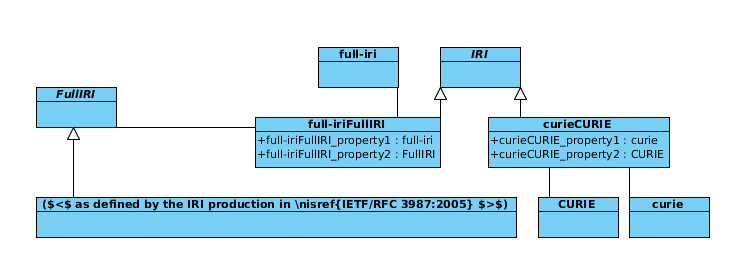
\includegraphics[scale=0.6]{mof/dia/dia7.png}

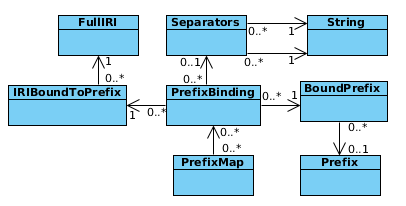
\includegraphics[scale=0.6]{mof/dia/dia8.png}

\ssclause{Abbreviating IRIs using CURIEs}\label{c:curies}

As IRIs tend to be long, and as syntactic mechanisms for abbreviating them have been standardized, 
it is \recommended that applications employ such mechanisms and support expanding abbreviatory
notations into full IRIs.  For specifying the \emph{semantics} of \DOL, this \IS assumes full IRIs 
everywhere, but the \DOL abstract \emph{syntax} adopts CURIEs (compact URI expressions) as an 
abbreviation mechanism, as it is the most flexible one that has been standardized to date.  

The CURIE abbreviation mechanism works by binding prefixes to IRIs.  A CURIE consists of a 
\emph{prefix}, which may be empty, and a \emph{reference}.  If there is an in-scope binding for the 
prefix, the CURIE is valid and expands into a full IRI, which is created by concatenating the IRI 
bound to the prefix and the reference.

\DOL adopts the CURIE specification of RDFa Core 1.1 \nisref{W3C/TR REC-rdfa-core:2013, Section 6} with the following changes:
\begin{itemize}
\item \DOL does not support the declaration of a ``default prefix'' mapping %\CLnote[type=q-aut]{Are such explanatory notes OK here? --- Yes}
(covering CURIEs such as \syntax{:name}).
\item \DOL does support the declaration  of a ``no prefix'' mapping (covering CURIEs such as 
\syntax{name}). If there is no explicit declaration for the ``no prefix'', it defaults to a 
context-sensitive expansion mechanism, which always prepends the \DOL library IRI (in the context of a 
structured OMS where named OMS are referenced) respectively the current OMS IRI (in the context of a basic
OMS) to a symbol name. Both the separator between the \DOL library and the OMS name and that between the 
OMS name and the symbol name can be declared (using the keyword \syntax{separators}), and both default to ``//''.

\item \DOL does not make use of the \syntax{safe\_curie} production.
\item \DOL does not allow binding a relative IRI to a prefix.
\item Concrete syntaxes of \DOL are encouraged but \notrequired to support CURIEs.
\end{itemize}

{CURIES are not required as 
a concession to having an RDF-based concrete syntax among the normative concrete syntaxes.  RDFa is 
the only standardized RDF serialization to support CURIEs so far.  Other serializations, such as 
RDF/XML or Turtle, support a subset of the CURIE syntax, whereas some machine-oriented 
serializations, including N-Triples, only support full IRIs.}

CURIEs can occur in any place where IRIs are allowed, as stated in \cref{c:iris}.  Informatively,\cbs 
the CURIE grammar supported by \DOL can be restated\cbe as follows:
\begin{lstlisting}[language=ebnf,escapeinside={()}]

CURIE         ::= MaybeEmptyCURIE -
MaybeEmptyCURIE ::= [Prefix] RefWithoutComma
RefWithoutComma ::= Reference - StringWithComma
StringWithComma ::= UChar* ',' UChar*
UChar         ::= ($<$ any Unicode \nisref{ISO/IEC 10646} character $>$) 
Prefix        ::= NCName ':'($<$ \rm see ``NCName'' in \nisref{W3C/TR REC-xml-names:2009}, Section 3 $>$)
Reference     ::= Path [Query] [Fragment]
Path          ::= ipath-absolute | ipath-rootless | ipath-empty($<$ \rm as defined in \nisref{IETF/RFC 3987} $>$)
Query         ::= '?' iquery($<$ \rm as defined in \nisref{IETF/RFC 3987} $>$)
Fragment      ::= '#' ifragment($<$ \rm as defined in \nisref{IETF/RFC 3987} $>$)
\end{lstlisting}

%\ednote{This is concrete syntax. Shouldn't it be moved to chapter \ref{{a:text-syntax}}? --- I have copied it there, altough this is code
%duplication.}

Note that outside the context of a basic OMS the prefix/reference separator of a CURIE is always the colon (\syntax{:}); only for serializations of OMS languages other than \DOL it may be redefined as stated in \cref{c:conform:serialization}.

Prefix mappings can be defined at the beginning of a \DOL library (specified in \cref{c:libraries}; 
these apply to all parts of the \DOL library, including basic OMS as clarified in \cref{c:map-ids}).  
%Their syntax is:

Bindings in a prefix map are evaluated from left to right.  Authors \shouldnot bind the same prefix twice, but if they do, the later binding wins.

\ssclause{Mapping identifiers in basic OMS to IRIs}\label{c:map-ids}

While \DOL uses IRIs as identifiers throughout, OMS languages do not necessarily do; for example:
\begin{itemize}
\item OWL \nisref{W3C/TR REC-owl2-syntax:2009, Section 5.5} does use IRIs.
\item Common Logic \nisref{ISO/IEC 24707:2007} supports them but does not enforce their use.
\item F-logic \cite{flogic} does not use them at all.
\end{itemize}
However, \DOL OMS mappings as well as 
%\CLnote[type=todo]{maybe clarify which ones, by checking the grammar for all occurrences of SymbolRef}
certain operations on OMS require making unambiguous references to non-logical symbols of basic OMS (\syntax{SymbolRef}).  Therefore, \DOL provides a function that maps global identifiers used within basic OMS to IRIs.  This mapping affects all non-logical symbol identifiers (such as class names in an OWL ontology), but not locally-scoped identifiers such as bound variables in Common Logic ontologies.  \DOL reuses the CURIE mechanism for abbreviating IRIs for this purpose (\cf \cref{c:curies}).

The IRI of a non-logical symbol identifier in a basic OMS $O$ is determined by the following function:
\begin{algorithmic}
  \REQUIRE $D$ is a \DOL library
  \REQUIRE $O$ is a basic OMS in serialization $S$
  \REQUIRE $\mathit{id}$ is the identifier in question, identifying a symbol in $O$ according to the specification of $S$
  \ENSURE $i$ is an IRI
  \IF{$\mathit{id}$ represents a full IRI according to the specification of $S$}
    \STATE $i\leftarrow\mathit{id}$
  \ELSE
    \STATE \COMMENT{first construct a pattern $\mathit{cp}$ for CURIEs in $S$, then match $\mathit{id}$ against that pattern}
    \IF{the declaration of \DOL-conformance of $S$ redefines the prefix/reference separator character $\mathit{cs}$ (cf.\ \cref{c:conform:serialization})}
      \STATE $\mathit{sep}\leftarrow \mathit{cs}$
    \ELSIF{$S$ forbids prefixed CURIEs}
      \STATE $\mathit{sep}\leftarrow\text{undefined}$
    \ELSE
      \STATE $\mathit{sep}\leftarrow\mathit{:}$ \COMMENT{the standard CURIE separator character}
    \ENDIF
    \STATE \COMMENT{The following statements construct a modified EBNF grammar of CURIEs; see \nisref{ISO/IEC 14977:1996} for EBNF, and \cref{c:curies} for the original grammar of CURIEs.}
    \IF{$\mathit{sep}$ is defined}
      \STATE $\mathit{cp}\leftarrow [ \mathit{NCName}, \mathit{sep} ] , \mathit{Reference}$
    \ELSE
      \STATE $\mathit{cp}\leftarrow \mathit{Reference}$
    \ENDIF 
    \IF{$\mathit{id}$ matches the pattern $\mathit{cp}$, where $\mathit{ref}$ matches $\mathit{Reference}$}
      \IF{the match succeeded with a non-empty $\mathit{NCName}$ $\mathit{pn}$}
        \STATE $p\leftarrow\mathit{concat}(pn, \mathit{:})$
      \ELSE
        \STATE $p\leftarrow\text{no prefix}$
      \ENDIF
      \IF{$O$ binds $p$ to an IRI $\mathit{pi}$ according to the specification of $S$}
        \STATE $\mathit{nsi}\leftarrow\mathit{pi}$
      \ELSE
        \STATE $P \leftarrow$ the innermost prefix map in $D$, starting from the place of $O$ inside $D$, and going up the abstract syntax tree towards the root of $D$
        \WHILE{$P$ is defined}
          \IF{$P$ binds $p$ to an IRI $\mathit{pi}$}
            \STATE $\mathit{nsi}\leftarrow\mathit{pi}$
            \STATE \textbf{break} out of the \textbf{while} loop 
          \ENDIF
          \STATE $P \leftarrow$ the next prefix map in $D$, starting from the place of the current $P$ inside $D$, and going up the abstract syntax tree towards the root of $D$
        \ENDWHILE
        \RETURN an error
      \ENDIF
      \STATE $i\leftarrow\mathit{concat}(\mathit{nsi}, \mathit{ref})$
    \ELSE
      \RETURN an error
    \ENDIF
  \ENDIF
  \RETURN $i$
\end{algorithmic}

This mechanism applies to basic OMS given inline in a \DOL library (\syntax{BasicOMS}), not to OMS in external documents (\syntax{NativeDocument}); the latter \shall be self-contained.

While CURIEs used for identifying parts of a \DOL library (\cf \cref{c:curies}) are merely syntactic 
sugar, the prefix map for a basic OMS is essential to determining the semantics of the basic OMS 
within the \DOL library.  Therefore, any \DOL serialization \shall provide constructs for expressing such 
prefix maps, even if the serialization does not support prefix maps otherwise.

%% ~\todonote[author=Christoph Lange,date=D:201111081514+01'00',type=todo]{somewhere we need to mention semantic annotations to embedded fragments in conforming OMS languages, \eg \%implied}



%% \sclause{Annotations}\label{s:annotations}

%% \todonote{this subclause will be moved to annex M}
%% ~\todonote[author=Christoph Lange,date=D:201108061340+02'00',type=todo]{Properly integrate this text from our LaRC 2011 paper} Annotations always have a subject, which is identified by an IRI. Where the given OMS language does not provide a way of assigning IRIs to a desired subject of an annotation (\eg if one wants to annotate an import in OWL), a library may employ RDF annotations that use XPointer or \nisref{IETF/RFC 5147} as a means of non-destructively referencing pieces of XML or text by URI.\footnote{We intend to utilize the extensibility of the XPointer framework by developing additional XPointer schemes, \eg for pointing to subterms of Common Logic sentences.}


\clause{\DOL Text Serialization}\label{a:text-syntax}

\sclause{Document Type}

\begin{description}
\item[MIME type] \mimetype{application/dol+text}
\item[Filename extension] .dol
\end{description}

\sclause{Concrete Syntax}\label{a:dol-text:concrete}

At several places, the concrete syntax uses the non-terminal
\syntax{'end'} to mark the end of a definition or declaration. Tools
may make this \syntax{'end'} optional. However, in this standard,\cbs
the \syntax{'end'} is not marked as optional,\cbe because it may be needed to effectively
disambiguate heterogeneous texts.

 
\ssclause{Documents}

\begin{lstlisting}[language=ebnf,escapeinside={()},morecomment={[l]{\%\%\ }}]

Document           ::= [PrefixMap] DOLLibrary | NativeDocument
DOLLibrary         ::= 'library' LibraryName Qualification LibraryItem*
NativeDocument     ::= ($<$) language and serialization specific ($>$) 
LibraryItem        ::= LibraryImport
                     | OMSDefinition
                     | NetworkDefinition
                     | MappingDefinition
                     | Qualification
LibraryImport      ::= 'import' LibraryName
Qualification      ::= LanguageQualification
                     | LogicQualification
                     | SyntaxQualification
LanguageQualification ::= 'language' LanguageRef
LogicQualification ::= 'logic' LogicRef
SyntaxQualification ::= 'serialization' SyntaxRef
LibraryName        ::= IRI
\end{lstlisting}


\begin{lstlisting}[language=ebnf,escapechar=+,morecomment={[l]{\%\%\ }}]

PrefixMap      ::= '%prefix(' PrefixBinding* ')%'
PrefixBinding  ::= BoundPrefix IRIBoundToPrefix [Separators]
BoundPrefix    ::= ':' | Prefix+$<$\rm see definition in \cref{c:curies}$>$\CLnote[type=q-aut]{I think that, in contrast to OWL Manchester, we can allow prefix names that match keywords of the \DOL syntax, as we are enclosing the whole prefix map into an annotation construct -- right?}+
IRIBoundToPrefix ::= '<' FullIRI '>'
Separators     ::= 'separators' SeparatorString SeparatorString
SeparatorString ::= SeparatorChar SeparatorChar*
SeparatorChar  ::= ipchar | gen-delims - '#'($<$ \rm as defined in \nisref{IETF/RFC 3987} $>$)
\end{lstlisting}


\cbs Note that the empty prefix (called ``no prefix'' in \nisref{W3C/TR REC-rdfa-core:2013, Section 6}) is denoted by a colon inside the prefix map, but it is omitted in CURIEs.\cbe  This is the style of the OWL Manchester syntax \cite{W3C:NOTE-owl2-manchester-syntax-20091027} but differs from the RDFa Core 1.1 syntax.

\vspace{1em}

\ssclause{Networks}

\begin{lstlisting}[language=ebnf,escapeinside={()},morecomment={[l]{\%\%\ }}]

NetworkDefinition  ::= 'network' NetworkName '='
                       [ConservativityStrength] Network
NetworkName        ::= IRI
Network            ::= NetworkElements [ExcludeExtensions]
NetworkElements    ::= NetworkElement ( ',' NetworkElement )*
NetworkElement     ::= [Id ':'] OMSOrMappingorNetworkRef
ExcludeExtensions  ::= 'excluding' ExcludedElement
                       ( ',' ExcludedElement )*
ExcludedElement    ::= IRI '->' IRI | OMSOrMappingorNetworkRef
OMSOrMappingorNetworkRef ::= IRI
Id                 ::= Letter LetterOrDigit*
\end{lstlisting}


\ssclause{OMS}\label{a:dol-text:OMS}

While in most cases the translation from concrete to abstract syntax
is obvious (the structure is largely the same),  both
\syntax{\%consistent} and \syntax{\%mcons} are translated to
\syntax{model-conservative}, while both \syntax{\%inconsistent} and
\syntax{\%notmcons} are translated to
\syntax{not-model-conservative}. Moreover, both \syntax{closed-world}
and \syntax{minimize} are translated to \syntax{minimize}.

                       
\begin{lstlisting}[language=ebnf,escapeinside={()},mathescape]

BasicOMS           ::= ($<$)language and serialization specific($>$) 
ClosableOMS        ::= BasicOMS | OMSRef [ImportName]
ExtendingOMS       ::= ClosableOMS
                     | MinimizeKeyword '{' ClosableOMS '}'
OMS                ::= ExtendingOMS
                     | OMS Minimization
                     | OMS Translation
                     | OMS Reduction
                     | OMS Approximation
                     | OMS Filtering
                     | OMS 'and' [ConservativityStrength] OMS
                     | OMS 'then' ExtensionOMS
                     | Qualification* ':' GroupOMS
                     | 'combine' NetworkElements [ExcludeExtensions]
                     | GroupOMS
Minimization       ::= MinimizeKeyword CircMin [CircVars]
MinimizeKeyword    ::= 'minimize'
                     | 'closed-world'
                     | 'maximize'
                     | 'free'
                     | 'cofree'
CircMin            ::= Symbol Symbol*
CircVars           ::= 'vars' (Symbol Symbol*)
GroupOMS           ::= '{' OMS '}' | OMSRef
Translation        ::= 'with' LogicTranslation* SymbolMap
                     | 'with' LogicTranslation LogicTranslation*
LogicTranslation   ::= 'translation' OMSLanguageTranslation
Reduction          ::= 'hide' LogicReduction* SymbolItems
                     | 'hide' LogicReduction LogicReduction*
                     | 'reveal' SymbolItems
LogicReduction     ::= 'along' OMSLanguageTranslation
SymbolItems        ::= Symbol ( ',' Symbol )*
SymbolMap          ::= GeneralSymbolMapItem ( ',' GeneralSymbolMapItem )*
Extraction         ::= 'extract' InterfaceSignature
                     | 'remove' InterfaceSignature
Approximation      ::= 'forget' InterfaceSignature ['keep' LogicRef]
                     | 'keep' InterfaceSignature ['keep' LogicRef]
                     | 'keep' LogicRef
Filtering          ::= 'select' BasicOMS | 'reject' BasicOMS
ExtensionOMS       ::= [ExtConservativityStrength]
                       [ExtensionName]
                       ExtendingOMS
ConservativityStrength ::= Conservative | '%mono' | '%wdef' | '%def'
ExtConservativityStrength ::= ConservativityStrength | '%implied'
Conservative       ::= '%ccons'
                     | '%mcons'
                     | '%notccons'
                     | '%notmcons'
                     | '%consistent'
                     | '%inconsistent'
InterfaceSignature ::= SymbolItems
ImportName         ::= '%(' IRI ')%'
ExtensionName      ::= '%(' IRI ')%'
OMSkeyword         ::= 'ontology'
                     | 'onto'
                     | 'specification'
                     | 'spec'
                     | 'model'
                     | 'oms'
OMSDefinition      ::= OMSkeyword OMSName '='
                       [ConservativityStrength] OMS 'end'
Symbol             ::= IRI
SymbolMapItem      ::= Symbol '|->' Symbol
GeneralSymbolMapItem ::= Symbol | SymbolMapItem
Sentence           ::= ($<$)an expression specific to an OMS language($>$) 
OMSName            ::= IRI
OMSRef             ::= IRI
LanguageRef        ::= IRI
LogicRef           ::= IRI
SyntaxRef          ::= IRI
LoLaRef            ::= LanguageRef | LogicRef
\end{lstlisting}


\begin{lstlisting}[language=ebnf,mathescape]

OMSLanguageTranslation ::= OMSLanguageTranslationRef | '->' LoLaRef
OMSLanguageTranslationRef ::= IRI
\end{lstlisting}


%\ednote{\%safe is more a statement about an import of a module, 
%and hence should be a statement in an OMS network. Recall:
%ModuleProperties     =  '\%safe' ; }

The above grammar allows for some grouping ambiguity when using operators in
OMS definitions. These ambiguities are resolved according to the following
list, listing operators in decreasing order of precedence:
\begin{itemize}
  \item \syntax{minimize}, \syntax{maximize}, \syntax{free}, and \syntax{cofree}. 
  \item \syntax{extract}, \syntax{forget}, \syntax{hide}, \syntax{keep},
    \syntax{reject}, \syntax{remove}, \syntax{reveal}, \syntax{select}, and
    \syntax{with}.
  \item \syntax{and}.
  \item \syntax{then}.
\end{itemize}
Multiple occurrences of the same operator are grouped in a left associative
manner. In all other cases operators on the same precedence level are not
implicitly grouped and have to be grouped explicitly. Omitting such an explicit
grouping results in a parse error.

\ssclause{OMS Mappings}\label{a:dol-text:mappings}
\index{alignment}
\begin{lstlisting}[language=ebnf,mathescape]

MappingDefinition  ::= InterpretationDefinition
                     | Entailment
                     | EquivalenceDefinition
                     | ModuleRelDefinition
                     | AlignmentDefinition
InterpretationDefinition ::= InterpretationKeyword
                             InterpretationName
                             [Conservative] ':'
                             InterpretationType 'end'
                     | InterpretationKeyword
                             InterpretationName
                             [Conservative] ':'
                             InterpretationType '='
                             LogicTranslation*
                             [SymbolMap] 'end'
                     | InterpretationKeyword
                             InterpretationName